\documentclass[conference]{IEEEtran}
\IEEEoverridecommandlockouts

% Core packages
\usepackage{cite}
\usepackage[T1]{fontenc}
\usepackage{hyperref}

% Math packages
\usepackage{amsmath,amssymb,amsfonts}
\usepackage{array,booktabs}

% Graphics and layout
\usepackage{graphicx}
\usepackage{subcaption}
\usepackage{float}
\usepackage{multirow}
\usepackage{multicol}
\usepackage{balance}

% Algorithm and code
\usepackage{algorithm}
\usepackage{algpseudocode} 
\usepackage{algorithmicx}
\usepackage{listings}

% Text and formatting
\usepackage{textcomp}
\usepackage{url}
\usepackage{enumitem}
\usepackage{caption} 
\usepackage{tcolorbox}
\usepackage{empheq}
\usepackage{varwidth}
\usepackage{balance}
\usepackage{todonotes}
\usepackage{flushend} 
\usepackage{stfloats}

\usepackage[ngerman,main=english]{babel}
 
% TikZ for diagrams
\usepackage{tikz}
\usetikzlibrary{arrows.meta,shapes,positioning}
\usetikzlibrary{calc,angles,quotes}

% --- Macro for drawing a 2D spherocylinder ---
% #1 = center coordinate
% #2 = rotation angle
% #3 = half-length
% #4 = radius
\newcommand{\drawSpherocyl}[4]{
    \begin{scope}[shift={(#1)},rotate=#2]
        \draw[line width=1pt,rounded corners=6pt] (-#3 + #4,#4) -- (#3 - #4,#4);
        \draw[line width=1pt,rounded corners=6pt] (-#3 + #4,-#4) -- (#3 - #4,-#4);
        \draw[line width=1pt,rounded corners=6pt] (#3 - #4,-#4) arc[start angle=-90,end angle=90,radius=#4];
        \draw[line width=1pt,rounded corners=6pt] (-#3 + #4,#4) arc[start angle=90,end angle=270,radius=#4];
        \fill [black] (#1) circle (2pt);
    \end{scope}
}



\hypersetup{hidelinks}
\DeclareMathAlphabet\mathbfcal{OMS}{cmsy}{b}{n}

% Macro for growth comparison row
\newcolumntype{M}[1]{>{\centering\arraybackslash}m{#1}}

\newcommand{\growthcomparisonrow}[6]{%
    #1 &
        \includegraphics[width=\linewidth]{figures/growth/#1_#2/#1_#2.#3.jpeg}
    &
        \includegraphics[width=\linewidth]{figures/growth/#1_#2/#1_#2.#4.jpeg}
    &
        \includegraphics[width=\linewidth]{figures/growth/#1_#2/#1_#2.#5.jpeg}
    &
        \includegraphics[width=\linewidth]{figures/growth/#1_#2/#1_#2.#6.jpeg}
    \\
}

\newcommand{\orientationcomparisonrow}[2]{%
    #1 &
        \includegraphics[width=\linewidth]{figures/orientation_comparisons/zoomed_images/hard_e#2_orient.jpeg}
    &   
        \includegraphics[width=\linewidth]{figures/orientation_comparisons/zoomed_images/soft_e#2_orient.jpeg}
    \\
}
 
\newcommand{\algorithmautorefname}{Algorithm}


\begin{document}

\title{Proliferating Cell Collectives: \\A Comparison of Hard and Soft Collision Models}

\author{
    \IEEEauthorblockN{Manuel Lerchner}
    \IEEEauthorblockA{
        \textit{Technical University of Munich}\\
        Munich, Germany}
}

\maketitle

\begin{abstract}
    This work compares hard (constraint-based) and soft (potential-based) collision models for simulating proliferating cell collectives by implementing both approaches within a unified computational framework. Building on the foundational work of Weady et al.~\cite{Weady2024}, we systematically benchmark their performance on bacterial colony growth simulations.

    Both approaches successfully reproduce experimentally observed patterns, including concentric rings and microdomain formation. However, they exhibit distinct computational and physical trade-offs. The hard model enforces strict non-overlap and stabilizes at timesteps approximately $30\times$ larger than the soft model ($\Delta t \approx 3 \times 10^{-4}$ h versus $10^{-5}$ h), at higher per-step computational cost. The soft model suffers from numerical stiffness and allows unphysical cell overlap, producing packing fractions exceeding 5 in colony centers compared to the hard model's realistic packing fraction of 0.9.

    Moreover, we introduce an adaptive timestepping algorithm based on the Courant-Friedrichs-Lewy condition, which dynamically selects stable timesteps tailored to the current colony state. Benchmarking reveals the hard model outperforms the soft model for small to moderate colonies ($R \leq 100$), while the soft model's superior scalability enables larger final colony sizes ($R \approx 200$) within practical runtimes.

    Despite microscopic differences in packing and stress distributions, both models yield comparable macroscopic patterns, suggesting colony-level behavior is robust to collision model details. The soft model provides an efficient, biologically plausible alternative for large-scale studies, while the hard model remains valuable when precise stress calculations or geometric integrity are required.
\end{abstract}

\begin{IEEEkeywords}
    collision models, constraint-based simulation, potential-based repulsion, bacterial colony growth, proliferating cell collectives, adaptive timestepping, pattern formation, computational performance, stress-sensitive growth, microdomain formation
\end{IEEEkeywords}

\section{Introduction}
\subsection{Biological Motivation}

The collective behaviors of biological entities, from microbial colonies to multicellular tissues, exemplify how local interactions among individual organisms can generate complex, large-scale structures and dynamics. These systems often exhibit emergent spatio-temporal patterns that arise from the interplay of cell growth, division, mechanical interactions, and local environmental feedback. Understanding such patterns is essential for comprehending fundamental biological processes and has applications ranging from biofilm formation to tissue engineering.

A particularly compelling example is found in bacterial colonies, where the spatial organization of cells encodes a record of growth dynamics and internal mechanical stresses. Continuous cell proliferation at the expanding periphery generates significant mechanical forces that accumulate in the densely packed interior~\cite{Wittmann2023}. These compressive stresses actively suppress growth in the colony center, creating a feedback loop: peripheral cells expand outward while internal cells remain densely packed and growth-limited. For bacterial species such as \textit{E. coli}, \textit{Bacillus subtilis}, and \textit{Proteus mirabilis}, as well as fungi like \textit{Setosphaeria rostrata} and \textit{Exserohilum turcicum}, this stress-dependent growth regulation produces the characteristic concentric ring patterns observed experimentally~\cite{YAMAZAKI2005136} (see \autoref{fig:exserohilum_turcicum}).

\begin{figure}[t]
    \centering
    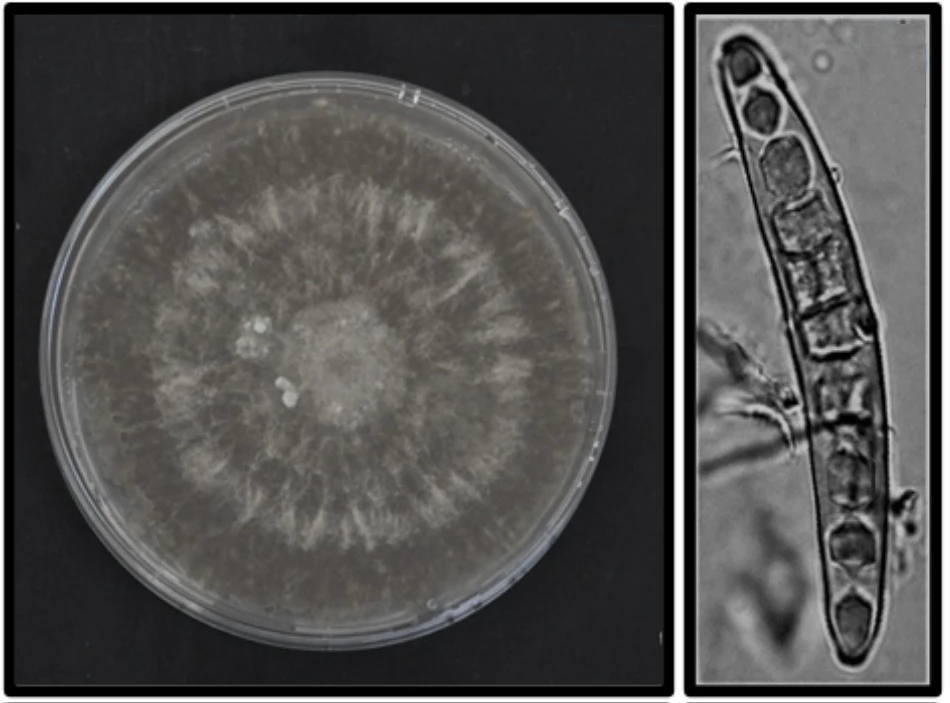
\includegraphics[width=\linewidth]{figures/real-bacteria/Exserohilum turcicum.png}
    \caption{Morphology of \textit{Exserohilum turcicum}. The left image displays a typical colony exhibiting concentric ring patterns, while the right image shows the elongated, rod-shaped morphology of individual cells. Source:~\cite{Bankole2023}.}
    \label{fig:exserohilum_turcicum}
\end{figure}

Computational modeling offers a powerful tool for dissecting these complex dynamics. To reproduce such emergent structures and understand their underlying mechanisms, models must accurately capture the dynamic interplay between cell growth and division, mechanical forces, and intercellular interactions. However, simulating dense, proliferating cell collectives presents significant computational challenges: the sheer number of cells in realistic colonies, combined with the need to resolve collisions accurately and efficiently across continuously changing configurations, creates a computational bottleneck. Different collision-handling approaches (rigid constraints versus soft repulsions) present distinct trade-offs between physical accuracy, numerical stability, and computational cost.

This work is directly motivated by these considerations and builds upon the pioneering computational framework developed by Weady et al.~\cite{Weady2024}, who demonstrated how to model bacterial colony growth while capturing stress-dependent feedback and pattern formation. We extend their work by systematically comparing two fundamentally different approaches to collision handling, examining their computational efficiency, physical fidelity, and suitability for large-scale simulations of proliferating cell collectives.



\section{Related Work}

\subsection{Collision Modeling Paradigms}

A critical computational challenge in agent-based models is the resolution of cell-cell collisions. Two primary paradigms exist for this purpose: potential-based (soft) and constraint-based (hard) models, each with distinct trade-offs in physical fidelity, computational cost, and numerical stability.

\begin{description}[style=nextline]
    \item[Potential-Based (Soft) Collision Models]
        Soft models manage cell interactions through repulsive forces defined by potentials such as Hertzian or Lennard-Jones functions. When cells overlap, these forces push them apart continuously. The primary advantage is computational efficiency: the calculations are local and embarrassingly parallelizable, enabling large-scale simulations. For instance, Warren et al.~\cite{Warren2019} demonstrated this by simulating millions of cells in three dimensions using a soft repulsion approach.

        However, soft models suffer from two key limitations. First, the stiffness of repulsive potentials creates numerical instability, requiring very small timesteps to maintain accuracy and prevent divergence. Second, the finite range of repulsive forces means cells behave as elastically deformable objects rather than rigid bodies, effectively reducing their geometric diameter below the intended size~\cite{Yan2019}. This deformation accumulates and can distort simulation results, particularly in dense regions.

    \item[Constraint-Based (Hard) Collision Models]
        Hard models enforce strict non-overlapping constraints, treating cells as geometrically rigid and impenetrable. Constraint-based methods are widely used in physics simulations~\cite{Tasora2008,Macklin2014,Li2021,Ferguson2021}, and have also been adapted for biological systems~\cite{Rudge2012,Weady2024,Yan2019}.

        The drawback is computational cost and increased complexity. Enforcing global non-overlap constraints requires iterative solvers that operate on large coupled systems of equations, creating a significant bottleneck. However, modern implementations~\cite{Yan2019} are able to efficiently reduce the numerical stiffness associated with soft models, allowing for much larger timesteps while maintaining geometric fidelity. The trade-off remains: higher cost per timestep due to constraint solving, but fewer timesteps needed overall.
\end{description}

\subsection{The Benchmarking Gap}

The two collision paradigms present fundamentally different trade-offs. Soft models offer computational simplicity and have been successfully scaled to millions of cells, but require small timesteps due to numerical stiffness and allow unphysical cell deformation. Hard models, particularly modern implementations~\cite{Yan2019}, eliminate stiffness and guarantee geometric rigidity, enabling timesteps $10$-$100\times$ larger. However, this advantage must be weighed against the substantially higher computational cost per timestep.

The central question remains unanswered: does the hard model's ability to take larger timesteps outweigh its higher per-step cost? This trade-off is especially critical in proliferating cell collectives, where exponentially increasing cell density intensifies collision resolution demands.

To our knowledge, a direct systematic comparison of these models is absent from the literature. Existing studies validate their chosen approach against experimental data, such as microscopy images, growth curves, and morphological features~\cite{Rudge2012,Weady2024,Blanchard2015,Ghosh2015,You2018,Warren2019,Khan_2024,You_2021,Valdez2025,Rudge2013,Langeslay_2023}, prioritizing biological accuracy over computational analysis. Few provide rigorous benchmarking of runtime, scalability, or numerical stability as colony density increases. Consequently, modelers lack clear guidance on which paradigm is more efficient for a given problem scale.

This work addresses this gap by implementing both models within a unified computational framework, enabling direct quantitative comparison of their performance across a range of colony sizes and densities.

\section{Cell Mechanics}

For many bacteria and fungal hyphae, approximating cells as rigid rods is a reasonable simplification that captures their elongated morphology while preserving the essential mechanics of cell-cell interactions and colony expansion. Although real cells exhibit some flexibility and deformability, this idealization effectively reproduces key emergent patterns observed experimentally~\cite{Rudge2012,Khan_2024,Rudge2013,Langeslay_2023,Ghosh2015}. This choice is well-supported by experimental observations and aligns with established practices in modeling microbial systems.

The spherocylinder geometry is particularly well-suited for capturing the dominant mechanical effects in dense cell collectives: it accommodates rotational interactions through contact, enables accurate force transmission along the cell body, and simplifies geometric contact calculations without sacrificing biological realism. Moreover, this representation scales well computationally, allowing simulations of large colonies without prohibitive memory or processing demands.

\subsection{Physical Cell Model}

Each cell is modeled as a spherocylinder (a rigid rod with hemispherical caps) characterized by a variable length $\ell$ and constant diameter $d$. This representation is widely used in cellular collective models~\cite{You2018, Weady2024, Blanchard2015, Warren2019, Ghosh2015} and closely matches the morphology of common bacteria and fungi such as \textit{E. coli} and \textit{Setosphaeria rostrata} (see \autoref{fig:exserohilum_turcicum}).

At bacterial length scales, the Reynolds number is extremely small ($\text{Re} \ll 1$), meaning that viscous forces dominate over inertia and bacteria move in a \textit{sticky} environment where they stop immediately after a force is applied~\cite{datta2024lifelowreynoldsnumber,Rudge2012}. The system is therefore governed by the overdamped Langevin equation:

\begin{equation} \label{eq:overdamped_langevin}
    \mathbf{u}_i = \frac{1}{\zeta \ell_i} \sum_j \mathbf{F}_{ij}, \quad
    \boldsymbol{\omega}_i = \frac{12}{\zeta \ell_i^3} \sum_j \mathbf{r}_{ij} \times \mathbf{F}_{ij}
\end{equation}

Here, $\mathbf{u}_i$ and $\boldsymbol{\omega}_i$ are the translational and angular velocities of cell $i$, $\mathbf{F}_{ij}$ is the force exerted on cell $i$ by cell $j$, $\zeta$ is the drag coefficient, and $\mathbf{r}_{ij}$ is the lever arm from the cell center to the contact point. Figure~\ref{fig:spherocylinder_model} illustrates the model and the forces and torques during collision.

\subsection{Cell Growth and Division}

Bacterial cells grow along their longitudinal axis according to the following model, adapted from~\cite{Weady2024SM}:

\begin{equation} \label{eq:growth}
    \dot{\ell} = \frac{\ell}{\tau} e^{-\lambda \sigma}
\end{equation}

where $\tau$ is a characteristic timescale, $\sigma$ is the compressive stress along the cell's main axis, and $\lambda$ is a stress sensitivity parameter. Stress on cell $i$ is computed by projecting contact forces onto the cell's longitudinal axis:

\begin{equation} \label{eq:stress}
    \sigma_i = \sum_{j} \frac{1}{2} \left| \hat{\mathbf{t}}_i \cdot \mathbf{F}_{ij} \right|
\end{equation}

where $\hat{\mathbf{t}}_i$ is the unit tangent vector along the cell's length.

For all simulations, cells begin with length $\ell_0 = 1$ and diameter $d = 0.5$. Division occurs when a cell reaches $\ell_{\text{crit}} = 2$, producing two daughter cells with lengths randomly sampled from $[0.98\ell_0, 1.02\ell_0]$ to avoid artificial synchronization of division events~\cite{Khan_2024}.

\subsection{Rotational Diffusion}

To account for Brownian motion, we apply a small random rotational perturbation to each cell at every timestep. This ensures cells gradually lose perfect alignment over time, which is important for realistic microdomain structure.


\begin{figure}[H]
    \centering


    \begin{tikzpicture}[line cap=round,line join=round,>=Stealth]

        % --- Variables ---
        \coordinate (xi) at (0.8,-0.5);
        \coordinate (xj) at (1.4,-1.8);

        \coordinate (x) at (-3,-0.5);
        \def\R{0.5}

        \drawSpherocyl{xi}{-10}{1.4}{\R}
        \drawSpherocyl{xj}{15}{1.3}{\R}

        \coordinate (contact) at  (1.85,-1.15);

        % Collision point
        \fill[black] (contact) circle (2pt) node[above right] {};

        % Force vector
        \draw[->,thick,red] (contact) -- ++($0.9*(-0.258,0.965)$) node[pos=0.9,left] {$\mathbf{F}_{ij}$};

        % Torque lever arm
        \draw[->,thick,blue,dashed] (xi) -- (contact) node[pos=0.2,below] {$\mathbf{r}_{ij}$};

        % Force vector
        \draw[->,thick,red] (contact) -- ++($0.8*(0.258,-0.965)$) node[pos=0.6,right] {$\mathbf{F}_{ji}$};

        % Torque lever arm
        \draw[->,thick,blue,dashed] (xj) -- (contact) node[pos=0.3,left] {$\mathbf{r}_{ji}$};



        % label at xi
        \node at (xi) [left] {$\mathbf{x}_i$};
        % label at xj
        \node at (xj) [below] {$\mathbf{x}_j$};


        \drawSpherocyl{x}{0}{2}{\R};

        % Add division constriction: two daughters forming
        \coordinate (left_daughter) at ($(x)+(-1,-1.25)$);
        \coordinate (right_daughter) at ($(x)+(1, -1.25)$);

        \drawSpherocyl{left_daughter}{0}{1}{\R};
        \drawSpherocyl{right_daughter}{0}{1}{\R};


        % label at x
        \node at (x) [below] {$\mathbf{x}$};
        % label at left daughter
        \node at (left_daughter) [below] {$\mathbf{x}_\text{left}$};
        % label at right daughter
        \node at (right_daughter) [below] {$\mathbf{x}_\text{right}$};

        \draw[<->,thick,dashed] ($(x) + (-2,1)$) -- ($(x) + (2,1)$) node[midway,above] {$2\ell_0$};

        \draw[<->,thick,dashed] ($(x) + (-1.5-\R-\R,-\R)$) -- ($(x) + (-1.5-\R-\R,\R)$) node[midway,left] {$d$};

        \draw[<->,thick,dashed] ($(right_daughter) + (-2.5-\R-\R,-\R)$) -- ($(right_daughter) + (-2.5-\R-\R,\R)$) node[midway,left] {$d$};

        \draw[<->,thick,dashed] ($(left_daughter) + (-1,-1)$) -- ($(left_daughter) + (1,-1)$) node[midway,below] {$\ell_0$};

        \draw[<->,thick,dashed] ($(right_daughter) + (-1,-1)$) -- ($(right_daughter) + (1,-1)$) node[midway,below] {$\ell_0$};



        % Resulting rotation around xi
        \draw[->,thick,orange]
        ($(xi)+(0.6,0.5)$) arc[start angle=0,end angle=160,radius=0.6]
        node[midway, below] {$\boldsymbol{\omega}_i$};


        % Resulting rotation around xj
        \draw[->,thick,orange]
        ($(xj)+(0.7,-0.5)$) arc[start angle=0,end angle=-150,radius=0.6]
        node[midway, above] {$\boldsymbol{\omega}_j$};

    \end{tikzpicture}
    \caption{Spherocylinder cell model. Contact forces $\mathbf{F}_{ij}$ (red) and lever arms $\mathbf{r}_{ij}$ (dashed blue) generate torques causing angular motion $\boldsymbol{\omega}$ (orange). Cell division occurs when a cell reaches critical length $2\ell_0$, producing two daughter cells of length $\ell_0$ in place of the parent cell.}
    \label{fig:spherocylinder_model}

\end{figure}

\section{Unified Computational Framework}

\subsection{Colony Representation}

Following Weady et al.~\cite{Weady2024SM}, the bacterial colony is represented by a global state vector $\mathbfcal{C} = [\dots, \mathbf{x}_n^\top, \mathbf{q}_n^\top, \dots]^\top \in \mathbb{R}^{7N}$, where $N$ is the number of cells. Each cell is represented by a 7-dimensional sub-vector consisting of a position vector $\mathbf{x}_n \in \mathbb{R}^3$ and a unit quaternion $\mathbf{q}_n \in \mathbb{R}^4$ representing its orientation. The lengths of all cells are stored separately in a vector $\boldsymbol{\ell} = [\dots, \ell_n, \dots]^\top \in \mathbb{R}^{N}$.

Quaternions are used instead of Euler angles or rotation matrices because they avoid singularities (gimbal lock), provide stable numerical integration over long simulations, and require less memory (4 components vs. 9 for rotation matrices).

\subsection{Colony Dynamics}

The translational and angular velocities of all cells in the colony from \autoref{eq:overdamped_langevin} are determined simultaneously by a force-velocity relationship $\mathbfcal{U} = \mathbfcal{M}^k \mathbfcal{F}$. Here, $\mathbfcal{F} \in \mathbb{R}^{6N}$ is the generalized force vector for the entire colony, containing both force and torque components for each cell. Similarly, $\mathbfcal{U} \in \mathbb{R}^{6N}$ is the generalized velocity vector containing the resulting translational and angular velocities. The components of these vectors are defined as:

\begin{equation}
    \mathbfcal{F} = [\mathbf{f}_1, \boldsymbol{\tau}_1, \dots, \mathbf{f}_N, \boldsymbol{\tau}_N]^\top, \quad
    \mathbfcal{U} = [\mathbf{u}_1, \boldsymbol{\omega}_1, \dots, \mathbf{u}_N, \boldsymbol{\omega}_N]^\top
\end{equation}

where, $\mathbf{f}_i = \sum_j \mathbf{F}_{ij}$ is the total force on cell $i$ due to all other cells $j$ in contact with it, and $\boldsymbol{\tau}_i = \sum_j \mathbf{r}_{ij} \times \mathbf{F}_{ij}$ is the total torque. The diagonal mobility matrix $\mathbfcal{M}^k$ at timestep $k$ encodes the drag coefficients for all cells based on their current lengths $\ell_i^k$:

\begin{equation}
    \mathbfcal{M}^k = \text{diag}\left(\frac{1}{\zeta \ell_1^k}\mathbf{I}_3, \frac{12}{\zeta {\ell_1^k}^3}\mathbf{I}_3, \dots \right) \in \mathbb{R}^{6N \times 6N}
\end{equation}

where $\mathbf{I}_3$ is the $3 \times 3$ identity matrix.

\subsection{State Integration}

The orientation quaternion $\mathbf{q}_i^k$ for each cell evolves according to the kinematic equation $\dot{\mathbf{q}}_i^k = \frac{1}{2} \boldsymbol{\omega}_i \otimes \mathbf{q}_i^k$, where $\otimes$ denotes quaternion multiplication. To integrate translational and rotational dynamics consistently, we introduce a mapping $\mathbfcal{G}^k$, which converts Cartesian translational and angular velocities from $\mathbb{R}^{6N}$ into corresponding changes in positions and quaternions in $\mathbb{R}^{7N}$ (See~\cite{Weady2024SM,Yan2022,Tasora2008}). Using $\mathbfcal{G}^k$, the colony's state is updated via explicit Euler integration:

\begin{equation} \label{eq:colony_update}
    \mathbfcal{C}^{k+1} = \mathbfcal{C}^k + \Delta t \, \mathbfcal{G}^k \mathbfcal{U} = \mathbfcal{C}^k + \Delta t \, \mathbfcal{G}^k \mathbfcal{M}^k \mathbfcal{F}
\end{equation}

This mapping applies the quaternion kinematics to all quaternion components of the colony and ensures the Euler integration respects both translational and rotational dynamics.

The distinction between hard and soft collision models lies solely in how the generalized force vector $\mathbfcal{F}$ is computed, the state update mechanism remains identical.

\subsection{Soft Collision Model}

The soft collision model treats cell-cell interactions through continuous, potential-based repulsive forces. When cells overlap, these forces smoothly increase, preventing significant interpenetration while allowing elastic deformation. This approach, is well-suited for simulating the soft, deformable nature of real biological cells and has been widely used in prior work~\cite{Warren2019, You2018,Blanchard2015,Ghosh2015,Khan_2024,You_2021,Valdez2025,Rudge2013,Langeslay_2023}.

We implement a Hertzian contact model, which describes elastic deformation between curved surfaces in contact. The repulsive elastic force exerted on cell $i$ by cell $j$ is:

\begin{equation} \label{eq:hertzian_contact_model}
    \mathbf{F}^{\text{elastic}}_{ij} = k_{cc} \sqrt{d} \, \delta^{3/2} \, \hat{\mathbf{n}}
\end{equation}

where $\delta$ is the overlap distance, $d$ is the cell diameter, $k_{cc}$ is an elastic constant, and $\hat{\mathbf{n}}$ is the unit normal vector at the contact point. The $\delta^{3/2}$ dependence is characteristic of Hertzian theory for elastic contacts and produces a nonlinear, smooth increase in force as overlap grows (see \autoref{fig:hertzian_contact_model}).

\subsubsection{Force Assembly}

The total force and torque on cell $n$ are computed by summing contributions from all pairwise elastic interactions and can be used to assemble the global force vector $\mathbfcal{F}$:

\begin{equation} \label{eq:force_assembly}
    \mathbf{f}_i         = \sum_{j \neq i} \mathbf{F}^{\text{elastic}}_{ij}, \qquad
    \boldsymbol{\tau}_i  = \sum_{j \neq i} \mathbf{r}_{ij} \times \mathbf{F}^{\text{elastic}}_{ij}
\end{equation}

\subsubsection{Model Parameters and Numerical Stability}

The elastic constant is defined as $k_{cc} = \frac{Y}{\zeta}$, where $Y$ is the cell's Young's modulus and $\zeta$ is the fluid drag coefficient. Using typical bacterial parameters ($Y \approx 4$ MPa and $\zeta \approx 200$ Pa$\cdot$h)~\cite{You2018, Blanchard2015}, we set $k_{cc} = 20000$ h$^{-1}$. This value is sufficiently large to prevent significant overlap between cells. However, the steep, nonlinear nature of the Hertzian force law creates numerical stiffness: cells can undergo rapid acceleration when overlap occurs, potentially causing large position changes within a single timestep. To maintain stability, an extremely small timestep ($\Delta t \sim 10^{-5}$ h) is required~\cite{Khan_2024, You2018, Blanchard2015} (See \autoref{fig:simulation_time_vs_dt}). This timestep restriction is a well-known limitation of soft collision models and creates a significant computational bottleneck for large colonies.

\begin{figure}[H]
    \centering
    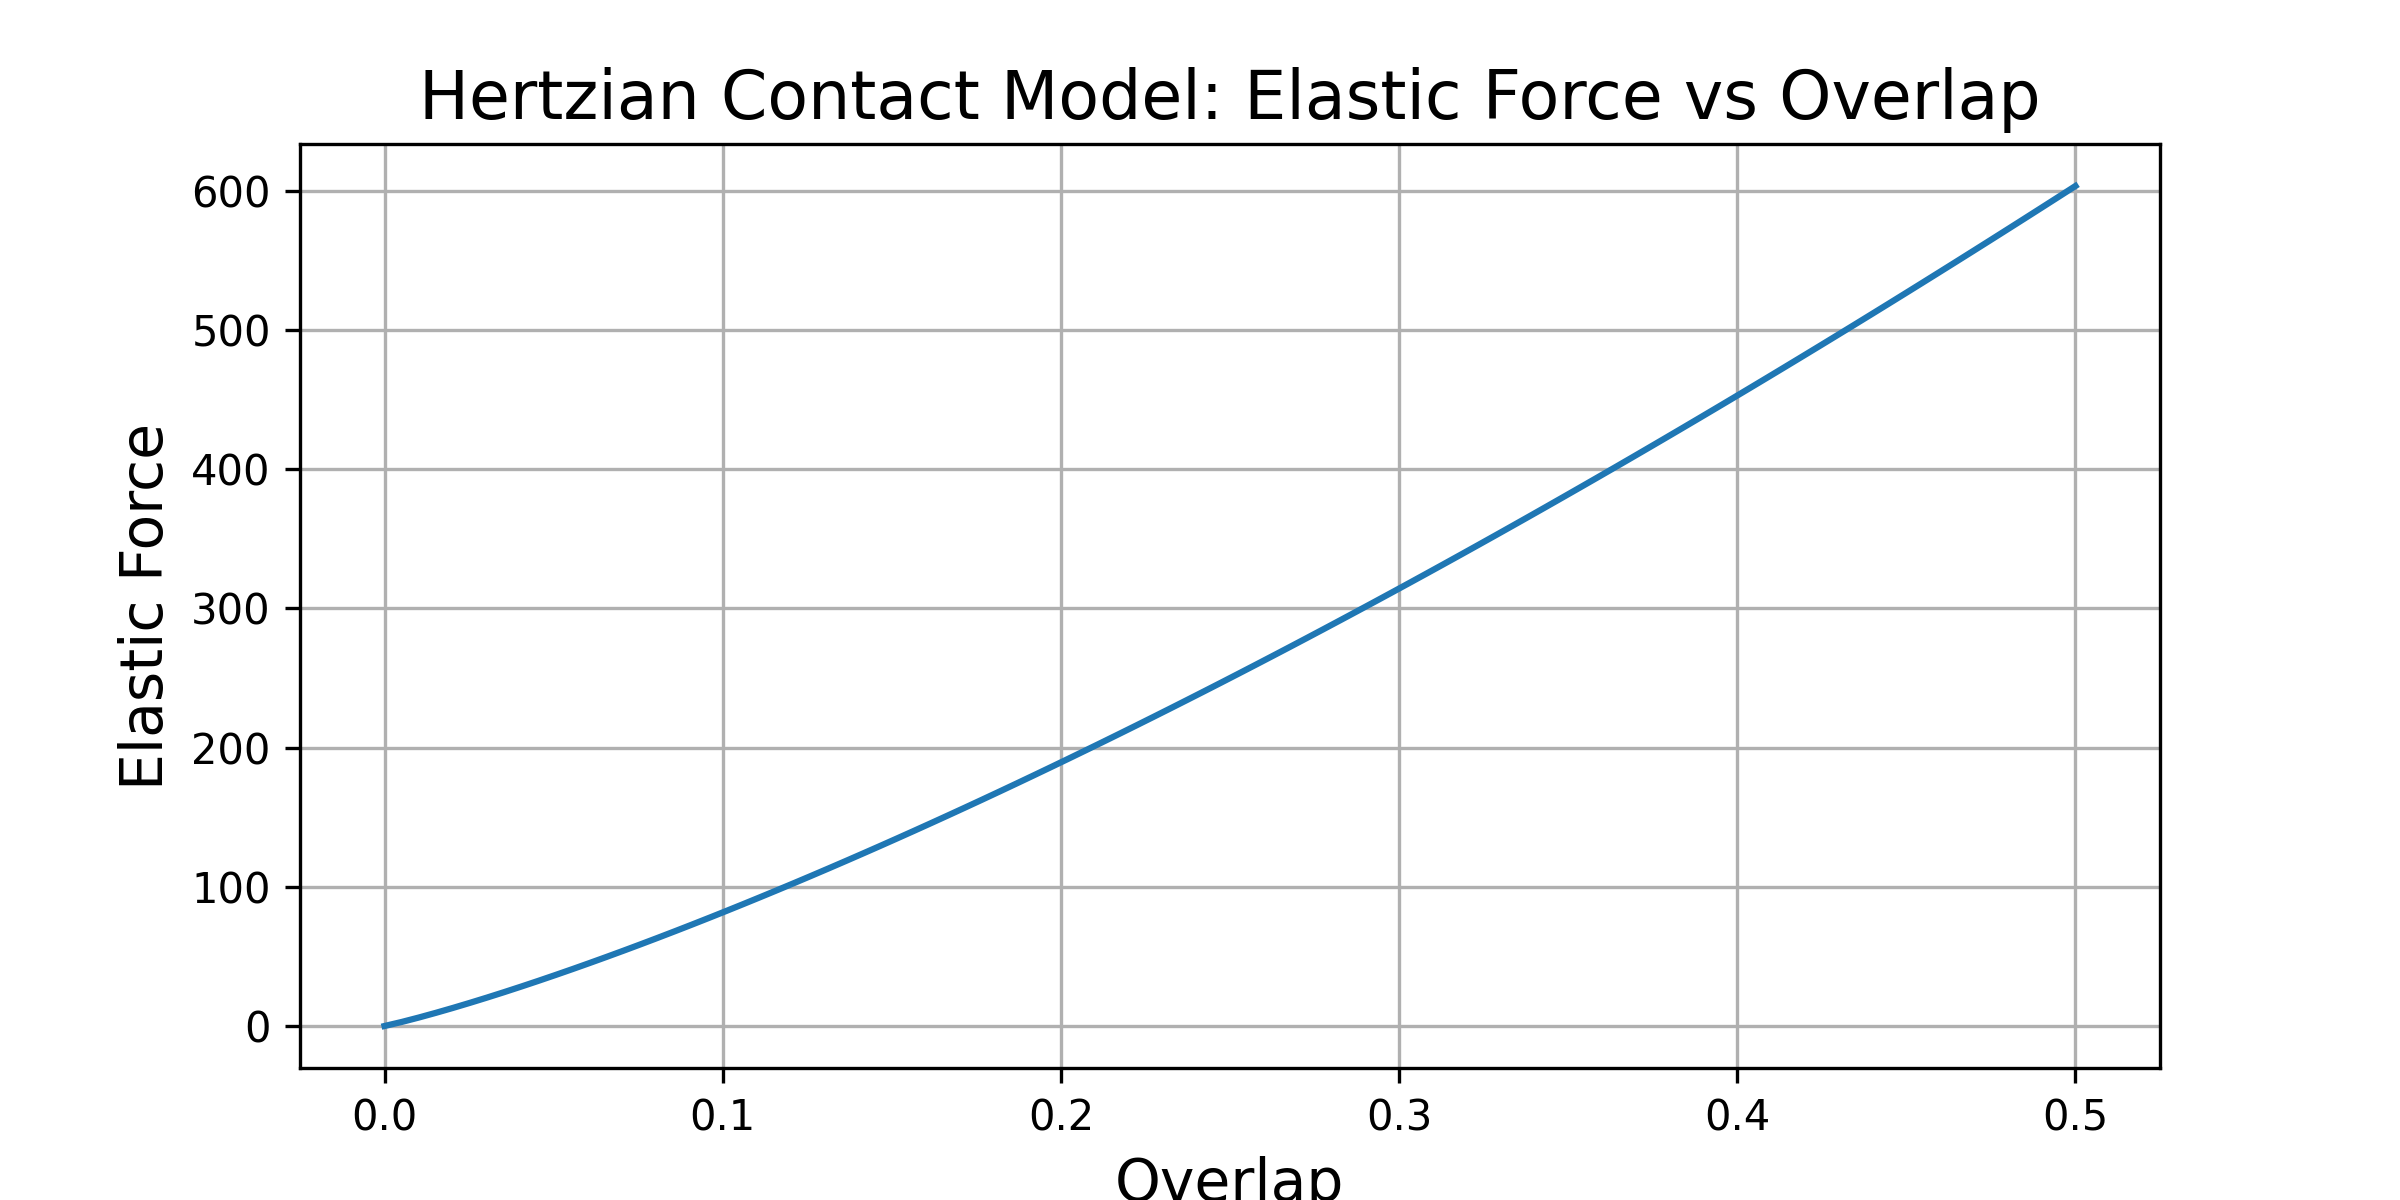
\includegraphics[width=\linewidth]{figures/hertzian_contact_model.png}
    \caption{Hertzian contact model. When two spherocylindrical cells overlap by a distance $\delta$, they experience a repulsive elastic force $\mathbf{F}^{\text{elastic}}$. The force acts along the normal vector $\hat{\mathbf{n}}$ at the contact point.}
    \label{fig:hertzian_contact_model}
\end{figure}

\subsection{Hard Collision Model}

The hard collision model enforces strict non-overlapping constraints between cells using a constraint-based method. For each nearby cell pair, a constraint $\alpha$ is defined based on the closest points on their surfaces, $\mathbf{y}_n$ and $\mathbf{y}_m$~\cite{Weady2024SM}. Unlike the soft model, which uses repulsive forces, the hard model determines contact forces via unknown scalar Lagrange multipliers $\gamma_\alpha$, which represent the magnitude of the impulse needed to prevent penetration.

The force on cell $n$ from constraint $\alpha$ is:
\begin{equation} \label{eq:constraint_force}
    \mathbf{F}^{\text{hard}}_{n\alpha} = \hat{\mathbf{n}}_\alpha \gamma_\alpha
\end{equation}

where $\hat{\mathbf{n}}_\alpha$ is the normal vector at the contact point. The total generalized force vector $\mathbfcal{F}$ for the colony depends linearly on the multipliers $\boldsymbol{\gamma} = [\dots, \gamma_\alpha, \dots]^\top \in \mathbb{R}^{C}$ and can be conveniently expressed in matrix form:
\begin{equation} \label{eq:force_as_function_of_multipliers}
    \mathbfcal{F}(\boldsymbol{\gamma}) = \mathbfcal{D} \boldsymbol{\gamma}
\end{equation}

where $\mathbfcal{D} \in \mathbb{R}^{6N \times C}$ is a sparse matrix consisting of contact normals and lever arms for all constraints. This matrix-vector product mimics the force assembly in Eq.~\ref{eq:force_assembly}, but uses the unknown multipliers $\boldsymbol{\gamma}$ instead of explicit force calculations. Similarly, the stress on each cell can also be expressed as a linear function of the multipliers:
\begin{equation} \label{eq:stress_as_function_of_multipliers}
    \boldsymbol{\sigma}(\boldsymbol{\gamma}) = \mathbfcal{L} \boldsymbol{\gamma}
\end{equation}

where $\mathbfcal{L} \in \mathbb{R}^{N \times C}$ encodes stress contributions from each constraint, such that the matrix-vector product mimics the stress calculation in Eq.~\ref{eq:stress},

\subsubsection{Constraint Conditions}

To ensure that solving for the multipliers $\boldsymbol{\gamma}$ leads to physically meaningful results, three key conditions must be satisfied:


\begin{enumerate}
    \item \textbf{Repulsive Forces:} $\boldsymbol{\gamma} \geq \mathbf{0}$. This ensures that the forces are repulsive, preventing cells from attracting each other.
    \item \textbf{No-Overlap:} $\mathbf{\Phi}^{k+1} \geq \mathbf{0}$ with $\mathbf{\Phi}^{k+1} = [\dots, \Phi_\alpha^{k+1}, \dots]^\top$. Here, $\mathbf{\Phi}^{k+1} \in \mathbb{R}^{C}$ is the vector of signed separation distances between the pairs of cells associated with each constraint $\alpha$ at timestep $k+1$. Each component $\Phi_\alpha^{k+1}$ is computed as the minimum separation distance between the associated cells. We use the robust geometric algorithm described by~\cite{Yan2019, GeometricTools} to compute these distances efficiently.
          A positive value $\Phi_\alpha^{k+1}$ indicates that the cells in the next iteration are separated, while a negative value indicates overlap. This condition enforces that no overlaps occur after the update.
    \item \textbf{Complementarity Condition:}  $\boldsymbol{\gamma}^\top \mathbf{\Phi}^{k+1} = \mathbf{0}$ (often written as $\boldsymbol{\gamma} \perp \mathbf{\Phi}^{k+1}$). This condition enforces that if two cells are in contact in the next iteration (i.e., $\Phi_\alpha^{k+1} = 0$), then a force may act in the current iteration to prevent overlap.
          Conversely, if two cells are separated in the next iteration (i.e., $\Phi_\alpha^{k+1} > 0$), no force should act in the current iteration (i.e., $\gamma_\alpha = 0$) in order to avoid force application at a distance.
\end{enumerate}

These conditions are often abbreviated as:
\begin{equation}
    \mathbf{0} \leq \boldsymbol{\gamma} \perp \mathbf{\Phi}^{k+1} \geq \mathbf{0}.
\end{equation}


The colony update rule and additional conditions combine to form a system where the future state $\mathbfcal{C}^{k+1}$ (and thus $\mathbf{\Phi}^{k+1}$) depends on $\boldsymbol{\gamma}$:

\begin{equation} \label{eq:colony_update_with_constraints}
    \begin{split}
        \mathbfcal{C}^{k+1} & = \mathbfcal{C}^k + \Delta t \mathbfcal{G}^k \mathbfcal{M}^k \mathbfcal{F}(\boldsymbol{\gamma}) \\
        \text{s.t.} \quad & \mathbf{0} \leq \boldsymbol{\gamma} \perp \mathbf{\Phi}^{k+1}(\boldsymbol{\gamma}) \geq \mathbf{0}.
    \end{split}
\end{equation}

\subsubsection{Linearization of the Constraint Condition}



The central challenge is that $\mathbf{\Phi}^{k+1}(\boldsymbol{\gamma})$ is a nonlinear function of the updated state $\mathbfcal{C}^{k+1}$ and is non-trivial to compute directly. Weady et al.~\cite{Weady2024SM} propose a linearization approach to approximate $\mathbf{\Phi}^{k+1}$ using a first-order Taylor expansion around the current state $\mathbfcal{C}^k$ and lengths $\boldsymbol{\ell}^k$. The change in $\mathbf{\Phi}$ in our model arises from two main effects:

\begin{enumerate}
    \item \textbf{Cell Motion:} All cell distances change due to the motion driven by collision forces. This is captured by the term $\dot{\mathbf{\Phi}^k}_{\text{motion}} = \frac{d \mathbf{\Phi}^k}{d \mathbfcal{C}} \frac{d \mathbfcal{C}}{dt} = (\nabla_{\mathbfcal{C}} \mathbf{\Phi}^k) \dot{\mathbfcal{C}}$.
    \item \textbf{Cell Growth:} Simultaneously, the cells grow, which also affects the cell distances. This is represented by $\dot{\mathbf{\Phi}^k}_{\text{growth}} = \frac{d \mathbf{\Phi}^k}{d \boldsymbol{\ell}} \frac{d \boldsymbol{\ell}}{dt} =-(\nabla_{\boldsymbol{\ell}} \mathbf{\Phi}^k) \dot{\boldsymbol{\ell}}$. (Note the negative sign, which arises because increasing cell lengths reduces the separation distances.)
\end{enumerate}

Combining these two effects, leads to the following approximation for $\mathbf{\Phi}^{k+1}$:

\begin{equation}\label{eq:phi_expanded}
    \small
    \begin{split}
        \mathbf{\Phi}^{k+1} & \approx \mathbf{\Phi}^k + \Delta t \Bigl( \dot{\mathbf{\Phi}}_{\text{motion}} + \dot{\mathbf{\Phi}}_{\text{growth}} \Bigr)\\
        & = \mathbf{\Phi}^k + \Delta t \Bigl( (\nabla_{\mathbfcal{C}} \mathbf{\Phi}^k) \dot{\mathbfcal{C}}^k - (\nabla_{\boldsymbol{\ell}} \mathbf{\Phi}^k) \dot{\boldsymbol{\ell}} \Bigr)\\
        & = \mathbf{\Phi}^k + \Delta t \Bigl( (\nabla_{\mathbfcal{C}} \mathbf{\Phi}^k) \mathbfcal{G}^k \mathbfcal{M}^k  \mathbfcal{F}(\boldsymbol{\gamma}) - (\nabla_{\boldsymbol{\ell}} \mathbf{\Phi}^k) \dot{\boldsymbol{\ell}} \Bigr)\\
        & \overset{\dagger}{=}
        \mathbf{\Phi}^k + \Delta t \Bigl( \mathbfcal{D}^\top \mathbfcal{M}^k  \mathbfcal{F}(\boldsymbol{\gamma})
        - (\nabla_{\boldsymbol{\ell}} \mathbf{\Phi}^k) \frac{\boldsymbol{\ell}}{\tau}
        e^{-\lambda \boldsymbol{\sigma}(\boldsymbol{\gamma})} \Bigr)\\
        & \overset{\ddagger}{=} \mathbf{\Phi}^k + \Delta t \Bigl( \mathbfcal{D}^\top \mathbfcal{M}^k \mathbfcal{D} \boldsymbol{\gamma} - \mathbfcal{L}^\top \frac{\boldsymbol{\ell}}{\tau} e^{-\lambda \mathbfcal{L} \boldsymbol{\gamma}} \Bigr)
    \end{split}
\end{equation}

Here ($\dagger$) we use the fact that $\mathbfcal{D}^\top = (\nabla_{\mathbfcal{C}} \mathbf{\Phi}) \mathbfcal{G}^k$, where $\mathbfcal{D}^\top$ is the Jacobian that maps velocities from the generalized coordinate space $\mathbb{R}^{6N}$ to changes in the signed distance functions $\mathbf{\Phi}$. Similarly, its transpose, $\mathbfcal{D}$ (which we introduced in \autoref{eq:force_as_function_of_multipliers}), maps forces from the constraint space back to the generalized coordinate space (See~\cite{Weady2024SM, Tasora2008} for details).

Moreover ($\ddagger$), we use a similar relation $\mathbfcal{L}^\top = \nabla_{\boldsymbol{\ell}} \mathbf{\Phi}^k \in \mathbb{R}^{C \times N}$, which defines the Jacobian mapping changes in cell lengths $\boldsymbol{\ell}$ to variations in the signed distance functions $\mathbf{\Phi}$~\cite{Weady2024SM}. Again, its transpose $\mathbfcal{L}$ (introduced in \autoref{eq:stress_as_function_of_multipliers}) maps stresses from the constraint space back to the length space.

\subsubsection{Nonlinear Complementarity Problem}

Substituting the approximation of $\mathbf{\Phi}^{k+1}$ from \autoref{eq:phi_expanded} into the constraint conditions of \autoref{eq:colony_update_with_constraints} yields a nonlinear complementarity problem (NCP) for $\boldsymbol{\gamma}$ which no longer depends on the unknown future state $\mathbfcal{C}^{k+1}(\boldsymbol{\gamma})$ and thus can be solved efficiently:
\begin{empheq}[box=\fbox]{equation} \label{eq:ncp_boxed}
    \small
    \begin{aligned}
         & \text{Find } \boldsymbol{\gamma} \ \text{such that} \\
         & \mathbf{0} \leq \boldsymbol{\gamma} \perp
        \mathbf{\Phi}^k
        + \Delta t \Biggl(
        \mathbfcal{D}^\top \mathbfcal{M}^k \mathbfcal{D} \boldsymbol{\gamma}
        - \mathbfcal{L}^\top
        \tfrac{\boldsymbol{\ell}}{\tau}
        e^{-\lambda \mathbfcal{L}\boldsymbol{\gamma}}
        \Biggr) \ge \mathbf{0}.
    \end{aligned}
\end{empheq}


\subsubsection{Energy Minimization Solution}

To solve this contact problem efficiently, we reframe it as an optimization problem\cite{CellModellerMaths}. We design a special function $E(\boldsymbol{\gamma})$ whose minimization resolves the contact forces. Physically, $E$ represents the work done by the contact forces and the system's internal energy:

\begin{equation} \label{eq:energy_function}
    \small
    \begin{aligned}
        E(\boldsymbol{\gamma}) =
        \boldsymbol{\gamma}^\top\mathbf{\Phi}^k
         & + \frac{\Delta t}{2} \boldsymbol{\gamma}^\top \mathbfcal{D}^\top \mathbfcal{M}^k \mathbfcal{D} \boldsymbol{\gamma} \\
         & + \mathbf{1}^\top \frac{\Delta t}{\lambda}
        \left( \frac{\boldsymbol{\ell}}{\tau} e^{-\lambda \mathbfcal{L} \boldsymbol{\gamma}} \right).
    \end{aligned}
\end{equation}

By construction, the gradient of this energy equals the linearized prediction:

\begin{equation}
    \begin{split}
        \nabla_{\boldsymbol{\gamma}} E & = \boldsymbol{\Phi}^k + \Delta t \mathbfcal{D}^\top \mathbfcal{M}^k \mathbfcal{D} \boldsymbol{\gamma} - \Delta t \mathbfcal{L}^\top \frac{\boldsymbol{\ell}}{\tau} e^{-\lambda \mathbfcal{L} \boldsymbol{\gamma}} \\
        & = \boldsymbol{\Phi}^{k+1}(\boldsymbol{\gamma})
    \end{split}
\end{equation}

Because $E(\boldsymbol{\gamma})$ is convex, it has a single, global minimum. We compute this minimum using a projected gradient method, which iteratively takes steps in the direction of the negative gradient and projects the result onto the feasible set $\boldsymbol{\gamma} \geq 0$ to enforce repulsive forces.

At the solution, the Karush-Kuhn-Tucker (KKT) conditions for this constrained minimum are exactly equivalent to our physical constraints:

\begin{enumerate}
    \item \textbf{Primal feasibility} ($\boldsymbol{\gamma}^* \geq 0$): We enforce this explicitly through a projection (\texttt{max} operator) during minimization, which prevents forces from becoming attractive. Physically, this ensures that contact forces only push cells apart according to the \textbf{Repulsive Forces} constraint.

    \item \textbf{Dual feasibility} ($\nabla E(\boldsymbol{\gamma}^*) \geq 0$): This must be true at the minimum. If the gradient pointed downhill ($\nabla E < 0$) at the solution, it would mean we could lower the energy further by increasing $\boldsymbol{\gamma}$, which contradicts that we are at a minimum. The only way to be at a minimum with the $\boldsymbol{\gamma} \geq 0$ constraint is if the gradient is zero (pointing nowhere) or positive (pointing uphill away from the boundary), meaning $\boldsymbol{\Phi}^{k+1} \geq 0$. Physically, this guarantees that no cells overlap after the update step in accordance with the \textbf{No-Overlap} constraint.

    \item \textbf{Complementary slackness} ($\boldsymbol{\gamma}^{*\top} \boldsymbol{\Phi}^{k+1} = 0$): This condition holds for a similar reason. If a contact force is active ($\gamma_\alpha > 0$), it means the system is free to adjust this force to find the minimum. At the true minimum, there can be no direction left to lower the energy. Therefore, for a non-zero force to be part of the final, optimal solution, the gradient (which equals $\Phi^{k+1}_\alpha = 0$) must be zero at that point, indicating the cells are in contact. Conversely, if $\gamma_\alpha = 0$, the gradient can be positive ($\Phi^{k+1}_\alpha > 0$) because we cannot go to lower energies by making $\gamma_\alpha$ more negative (as it is forbidden). Thus, the product $\gamma_\alpha \Phi^{k+1}_\alpha = 0$ for each contact $\alpha$, leading to the overall complementary slackness condition. Physically, this means forces act only where cells are touching. Separated cells never experience any repulsive force, satisfying the \textbf{Complementarity Condition}.
\end{enumerate}

Thus, the unique global minimizer $\boldsymbol{\gamma}^*$ resolves all contacts according to the physical laws of rigid-body interactions. This equivalence between the KKT conditions of a convex optimization problem and a complementarity problem is a well-known result in optimization theory~\cite{Nocedal2006} and is widely used in constraint-based physics simulations~\cite{Yan2022,Tasora2008, Yan2019, Li2021, Weady2024SM,Rudge2012,Macklin2014,Ferguson2021}.

\subsubsection{Numerical Solution}

We solve the constrained optimization using the Barzilai-Borwein projected gradient descent method (BBPGD)~\cite{BBPGD}, as implemented in~\cite{Weady2024SM,Yan2019}. This method is particularly well-suited for large-scale constrained optimization problems due to its computational efficiency and scalability. The algorithm iterates until a convergence criterion is met, producing $\boldsymbol{\gamma}^*$, which is then used to compute $\mathbfcal{F} = \mathbfcal{D}\boldsymbol{\gamma}^*$ and update the colony state via Eq.~\ref{eq:colony_update}.

Following Weady et al.~\cite{Weady2024SM}, we use a convergence tolerance of $\epsilon = 10^{-3}$, which directly corresponds to the maximum permissible overlap of any cell pair after the update step. This approach ensures that the residual computed by the algorithm has a clear physical interpretation, allowing us to control the accuracy of the simulation in terms of actual cell overlaps.

\subsubsection{Limitations of the Linearization}

A fundamental limitation of the linearization is that orthogonal motions, specifically rotations about contact points and translations parallel to the contact plane, are unconstrained within the linear approximation. Consequently, even after the BBPGD algorithm converges to the specified tolerance $\epsilon$, residual overlaps may still be present that violate the non-overlap constraint~\cite{Weady2024SM}.

To address this limitation, Weady et al.~\cite{Weady2024SM} developed the recursively generated linear complementarity problem (ReLCP) method. After each BBPGD convergence, ReLCP identifies any remaining overlaps by examining all pairwise cell distances, generates new constraints for these violations, and re-solves the complementarity problem with the augmented constraint set. This process iterates until all cell overlaps fall below the tolerance $\epsilon = 10^{-3}$. This hierarchical approach ensures that the non-overlap condition is strictly enforced, even in the presence of complex contact geometries and coupled motions (see \autoref{fig:bbpgd_residual}). The iterative refinement procedure typically converges within a small number of iterations, making it computationally tractable for most simulations~\cite{Weady2024SM}.

Nevertheless, this approach still requires a sufficiently small timestep $\Delta t \sim 5 \times 10^{-4}$ h (see \autoref{fig:simulation_time_vs_dt}) to ensure that cells do not move excessively~\cite{Yan2022}. When cells move too far within a single timestep, new overlaps can be generated that the linearization fails to capture during the current iteration, preventing constraint resolution. In practice, this causes the BBPGD method to fail to converge, or ReLCP to be unable to resolve all overlaps within a reasonable number of iterations, resulting in simulation failure.

Despite this computational restriction, the hard model's timestep requirement is less severe than the soft model's, though it still represents a significant computational bottleneck for large multicellular colonies with thousands or millions of cells.

\section{Implementation}

All simulations in this paper were performed with a custom C++ framework designed for large-scale simulations of proliferating cell collectives. The framework leverages distributed-memory parallel computing and standard HPC libraries to achieve scalability, enabling simulations of hundreds of thousands of cells across hundreds of CPU cores. The implementation combines concepts from Weady et al.~\cite{Weady2024SM} and similar frameworks~\cite{Tasora2008,Yan2019}.

\subsection{Distributed Computing Architecture}

The core architecture is built on two foundational libraries:
\begin{itemize}
    \item \textbf{PETSc}~\cite{petsc-web-page}: Used as a backend for distributed vectors and sparse matrices. PETSc partitions data across MPI processes and transparently handles inter-process communication for global operations (e.g., matrix-vector products, reductions).
    \item \textbf{MPI}: Underlies all inter-process communication, including ghost-cell exchanges at domain boundaries to maintain consistent collision handling across partitions.
\end{itemize}

Built on these abstractions, the framework implements the full physics pipeline, including both the ReLCP solver for the hard collision model and the soft collision model.

\subsection{Collision Handling Pipeline}

Collisions are processed through a unified pipeline designed to decouple geometry from physics. The process consists of two phases: broad-phase detection using a spatial grid (reducing neighbor searches to $O(N)$) and narrow-phase detection that computes exact contact points and geometric information. For each collision detected, the framework assembles a standardized data structure containing contact points, normals, and lever arms. This structure is passed to either the hard or soft collision model, which computes the resulting forces and torques. This abstraction allows seamless switching between collision models without altering the overall simulation flow.

Each collision detector call generates a single constraint per neighboring cell-pair within a threshold distance $d = 0.5$. As this threshold is larger than zero, it captures both overlapping and closely adjacent cells. This overapproximation is crucial for the stability in the hard model. For the soft model, those non-overlapping cell-pairs contribute no forces (since $\delta < 0$), while for the hard model they provide additional global information that improves constraint resolution. Ideally, constraints would be constructed between all cell pairs regardless of distance, but for computational efficiency only nearby cells are considered~\cite{Yan2019, Yan2022}.

\subsection{Adaptive Timestepping}

To enhance stability and convergence, particularly for fast-moving cells that might overlap significantly within a timestep, we employ an adaptive timestepping scheme. To our knowledge, this approach has not been implemented in comparable engines. As shown in \autoref{fig:simulation_time_vs_dt}, the method quickly converges to a stable maximum $\Delta t$ for both collision models while adapting dynamically throughout the simulation. It allows finer precision when needed and can even increase $\Delta t$ in cases where motion is limited, such as dense colonies with high $\lambda$ where internal cells are effectively immobile due to mechanical stress.

The adaptive timestep strategy (outlined in \autoref{alg:adaptive_dt}) is based on the Courant-Friedrichs-Lewy (CFL) condition~\cite{Courant1928}, which provides a stability criterion linking temporal and spatial resolution:

\begin{equation}
    \text{CFL} = \frac{u \, \Delta t}{\Delta x} \leq C_{\text{max}}.
\end{equation}

For our cell-based system, we define a characteristic velocity scale $u_m$ as the median of all cell velocities (including growth rates) and a characteristic spatial scale $\Delta x$ as the solver tolerance $\varepsilon = 10^{-3}$, which controls the maximum allowable displacement per step. Enforcing that cells move no more than half this tolerance yields:

\begin{equation} \label{eq:cfl_dt}
    \Delta t = \frac{0.5 \, \varepsilon}{u_m}.
\end{equation}

This directly bounds cell motion between successive updates, preventing excessive overlap and maintaining numerical stability in both collision models.

\begin{algorithm}[H]
    \caption{Adaptive Timestep Control}
    \label{alg:adaptive_dt}
    \begin{algorithmic}[1]
        \Require Particle set $\{p_i\}$ with velocities $v_i$ and growth rates $\dot{\ell_i}$, current timestep $\Delta t$, solver tolerance $\varepsilon$, smoothing factor $\alpha$.
        \Ensure Updated timestep $\Delta t$.

        \State Compute characteristic velocity $u_i = \|v_i\| + \dot{\ell_i}$ for each particle.
        \State Estimate system median velocity $u_m$.
        \State Determine $\Delta t^*$ using~\autoref{eq:cfl_dt}.
        \State Smooth the timestep change to avoid oscillations: $\Delta t_{\text{new}} = (1 - \alpha)\Delta t + \alpha \Delta t^*$ with $\alpha = 0.01$.
        \State Clamp $\Delta t_{\text{new}}$ within 20\% of current $\Delta t$ to prevent abrupt changes.
        \State Update simulation timestep: $\Delta t \gets \Delta t_{\text{new}}$.
    \end{algorithmic}
\end{algorithm}

\subsection{Simulation Output and Availability}

Simulation results are written in VTK format for visualization with ParaView~\cite{ahrens2005paraview}. All cell attributes, such as positions, orientations, lengths, stresses, growth rates, and contact forces, are periodically saved to disk, enabling comprehensive post-processing and detailed analysis.

The full simulation framework, including all features and implementations described in this work, is openly available on GitHub at \url{https://github.com/manuellerchner/MicrobeGrowthSim-IDP}.

\newpage

\section{Pattern Formation Analysis}

\subsection{Concentric Ring Patterns}

We validate both implementations by reproducing concentric ring patterns that arise under stress-sensitive growth, as reported in~\cite{Weady2024}. As shown in \autoref{fig:pattern_formation}, both models successfully produce qualitatively similar ring structures, demonstrating that the core mechanics of growth and mechanical feedback are effectively captured by both collision handling approaches.

The effect of $\lambda$ on pattern formation is consistent across both models. At very low stress-sensitivity ($\lambda = 10^{-4}$), no clear rings form even at the maximum simulated colony radius of 100, since growth inhibition is too weak to generate significant stress gradients. At intermediate sensitivity ($\lambda = 10^{-3}$), distinct concentric rings emerge early in the simulation and persist as the colony expands, with ring spacing determined by the balance between growth and stress. At high sensitivity ($\lambda = 10^{-2}$), an initially formed ring quickly dissipates as cells reorient to random orientations and growth nearly ceases due to strong mechanical inhibition throughout most of the colony.

Despite these qualitatively similar outcomes, visual differences emerge between the models. The soft model produces visibly denser patterns with a fuzzy appearance due to allowable cell overlap, while the hard model yields sharper, more sparsely looking rings. Nevertheless, macroscopic features, such as number of rings, spacing, and colony expansion rate, remain comparable between the two models, suggesting that colony-level pattern formation is robust to the details of collision handling.

\begin{figure*}[p]
    \centering

    % % Lambda = 10^-2 comparison

    Growth Comparison $\lambda=10^{-2}$
    \begin{tabular}{r M{0.2\textwidth} M{0.2\textwidth} M{0.2\textwidth} M{0.2\textwidth}}
        \growthcomparisonrow{hard}{e-2}{0055}{0100}{0150}{0199}
        \growthcomparisonrow{soft}{e-2}{0055}{0100}{0150}{0200}
    \end{tabular}
    % Lambda = 10^-3 comparison

    Growth Comparison $\lambda=10^{-3}$
    \begin{tabular}{r M{0.2\textwidth} M{0.2\textwidth} M{0.2\textwidth} M{0.2\textwidth}}
        \growthcomparisonrow{hard}{e-3}{0052}{0100}{0150}{0198}
        \growthcomparisonrow{soft}{e-3}{0048}{0110}{0149}{0187}
    \end{tabular}

    % Lambda = 10^-4 comparison

    Growth Comparison $\lambda=10^{-4}$
    \begin{tabular}{r M{0.2\textwidth} M{0.2\textwidth} M{0.2\textwidth} M{0.2\textwidth}}
        \growthcomparisonrow{hard}{e-4}{0051}{0100}{0140}{0192}
        \growthcomparisonrow{soft}{e-4}{0048}{0105}{0134}{0198}
    \end{tabular}

    \caption{Comparison of pattern formation between hard and soft collision models at similar colony sizes. Each row shows the colony evolutions up to a maximum colony radius of 100. The color indicates the length of the cells (short cells are darker, longer cells are lighter). Clear concentric ring pattern are visible for both models at $\lambda = 10^{-3}$ confirming the results from~\cite{Weady2024}.}
    \label{fig:pattern_formation}
\end{figure*}

\subsection{Cell Density and Local Packing Fraction}

The most striking difference between the models emerges in cell packing density (see \autoref{fig:dense_packing_comparison}). The soft model exhibits significantly denser packing in the colony center, decreasing radially outward (see \autoref{fig:radial_distribution_packing_fraction}). For very low stress-sensitivity ($\lambda = 10^{-4}$), local packing fractions reach values of 5, far exceeding the maximum possible for rigid spherocylinders. In contrast, the hard model maintains approximately constant, and physically realistic, packing density ($\sim 0.9$) throughout the colony, as non-overlap constraints immediately propagate any interior overlaps outward.

The unphysical packing fraction arises because the soft model relies on local pairwise forces that cannot fully propagate stress to the colony edge, combined with a numerical timestep too large to resolve all collisions. Figure~\ref{fig:max_overlap_simulation} quantifies this effect: the soft model's maximum cell overlap steadily increases throughout the simulation, reaching nearly complete interpenetration by the end. In contrast, the hard model maintains maximum overlap near the solver tolerance $\epsilon = 10^{-3}$ by enforcing strict non-overlap constraints.

A contributing factor to this excessive overlap is the adaptive timestep method (see \autoref{alg:adaptive_dt}), which bases $\Delta t$ on cell velocities but not on current overlap. Once cells begin overlapping, they can continue doing so as long as velocities remain low. A more sophisticated scheme could consider maximum overlap when adjusting $\Delta t$, though this remains as future work.

\begin{figure}[H]
    \centering
    \begin{subfigure}[b]{0.49\columnwidth}
        \centering
        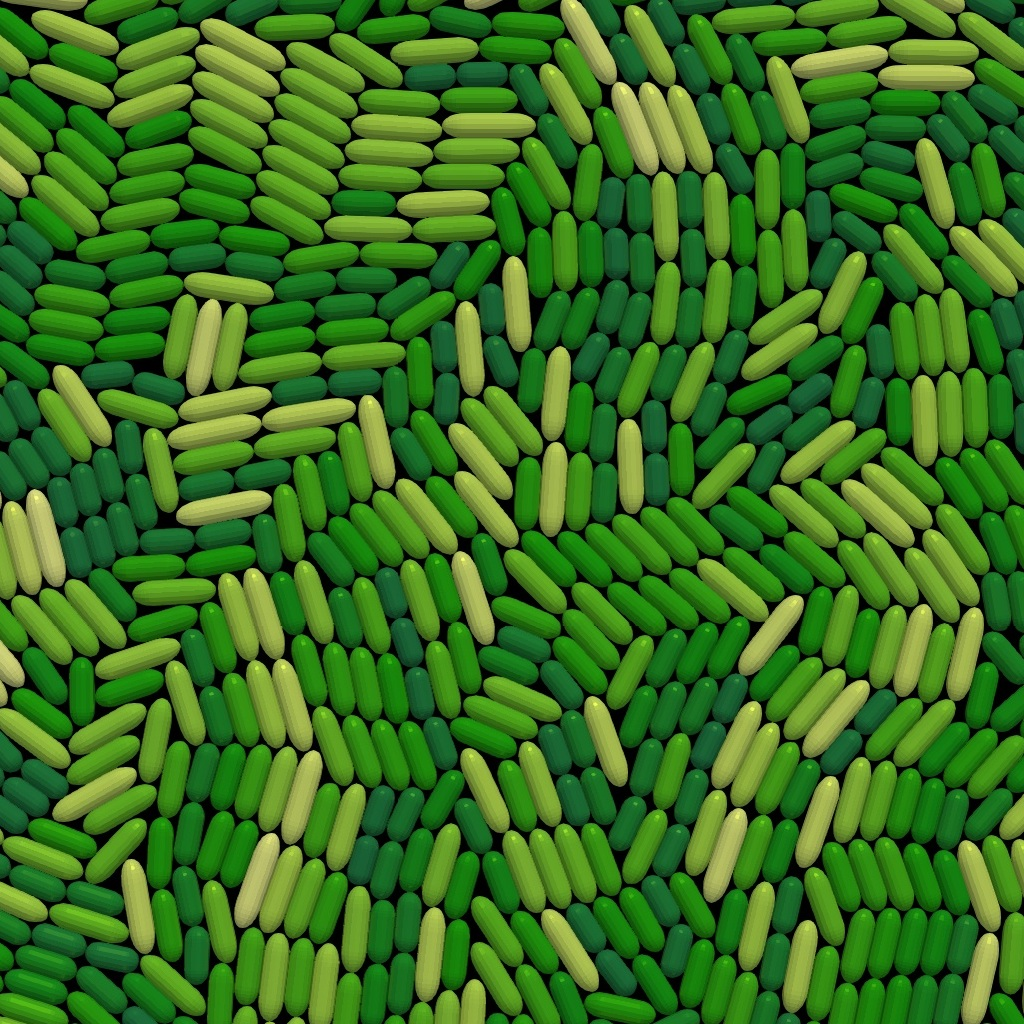
\includegraphics[width=\linewidth]{figures/comparison_plots/density_hard.jpeg}
        \caption{Hard model}
    \end{subfigure}
    \begin{subfigure}[b]{0.49\columnwidth}
        \centering
        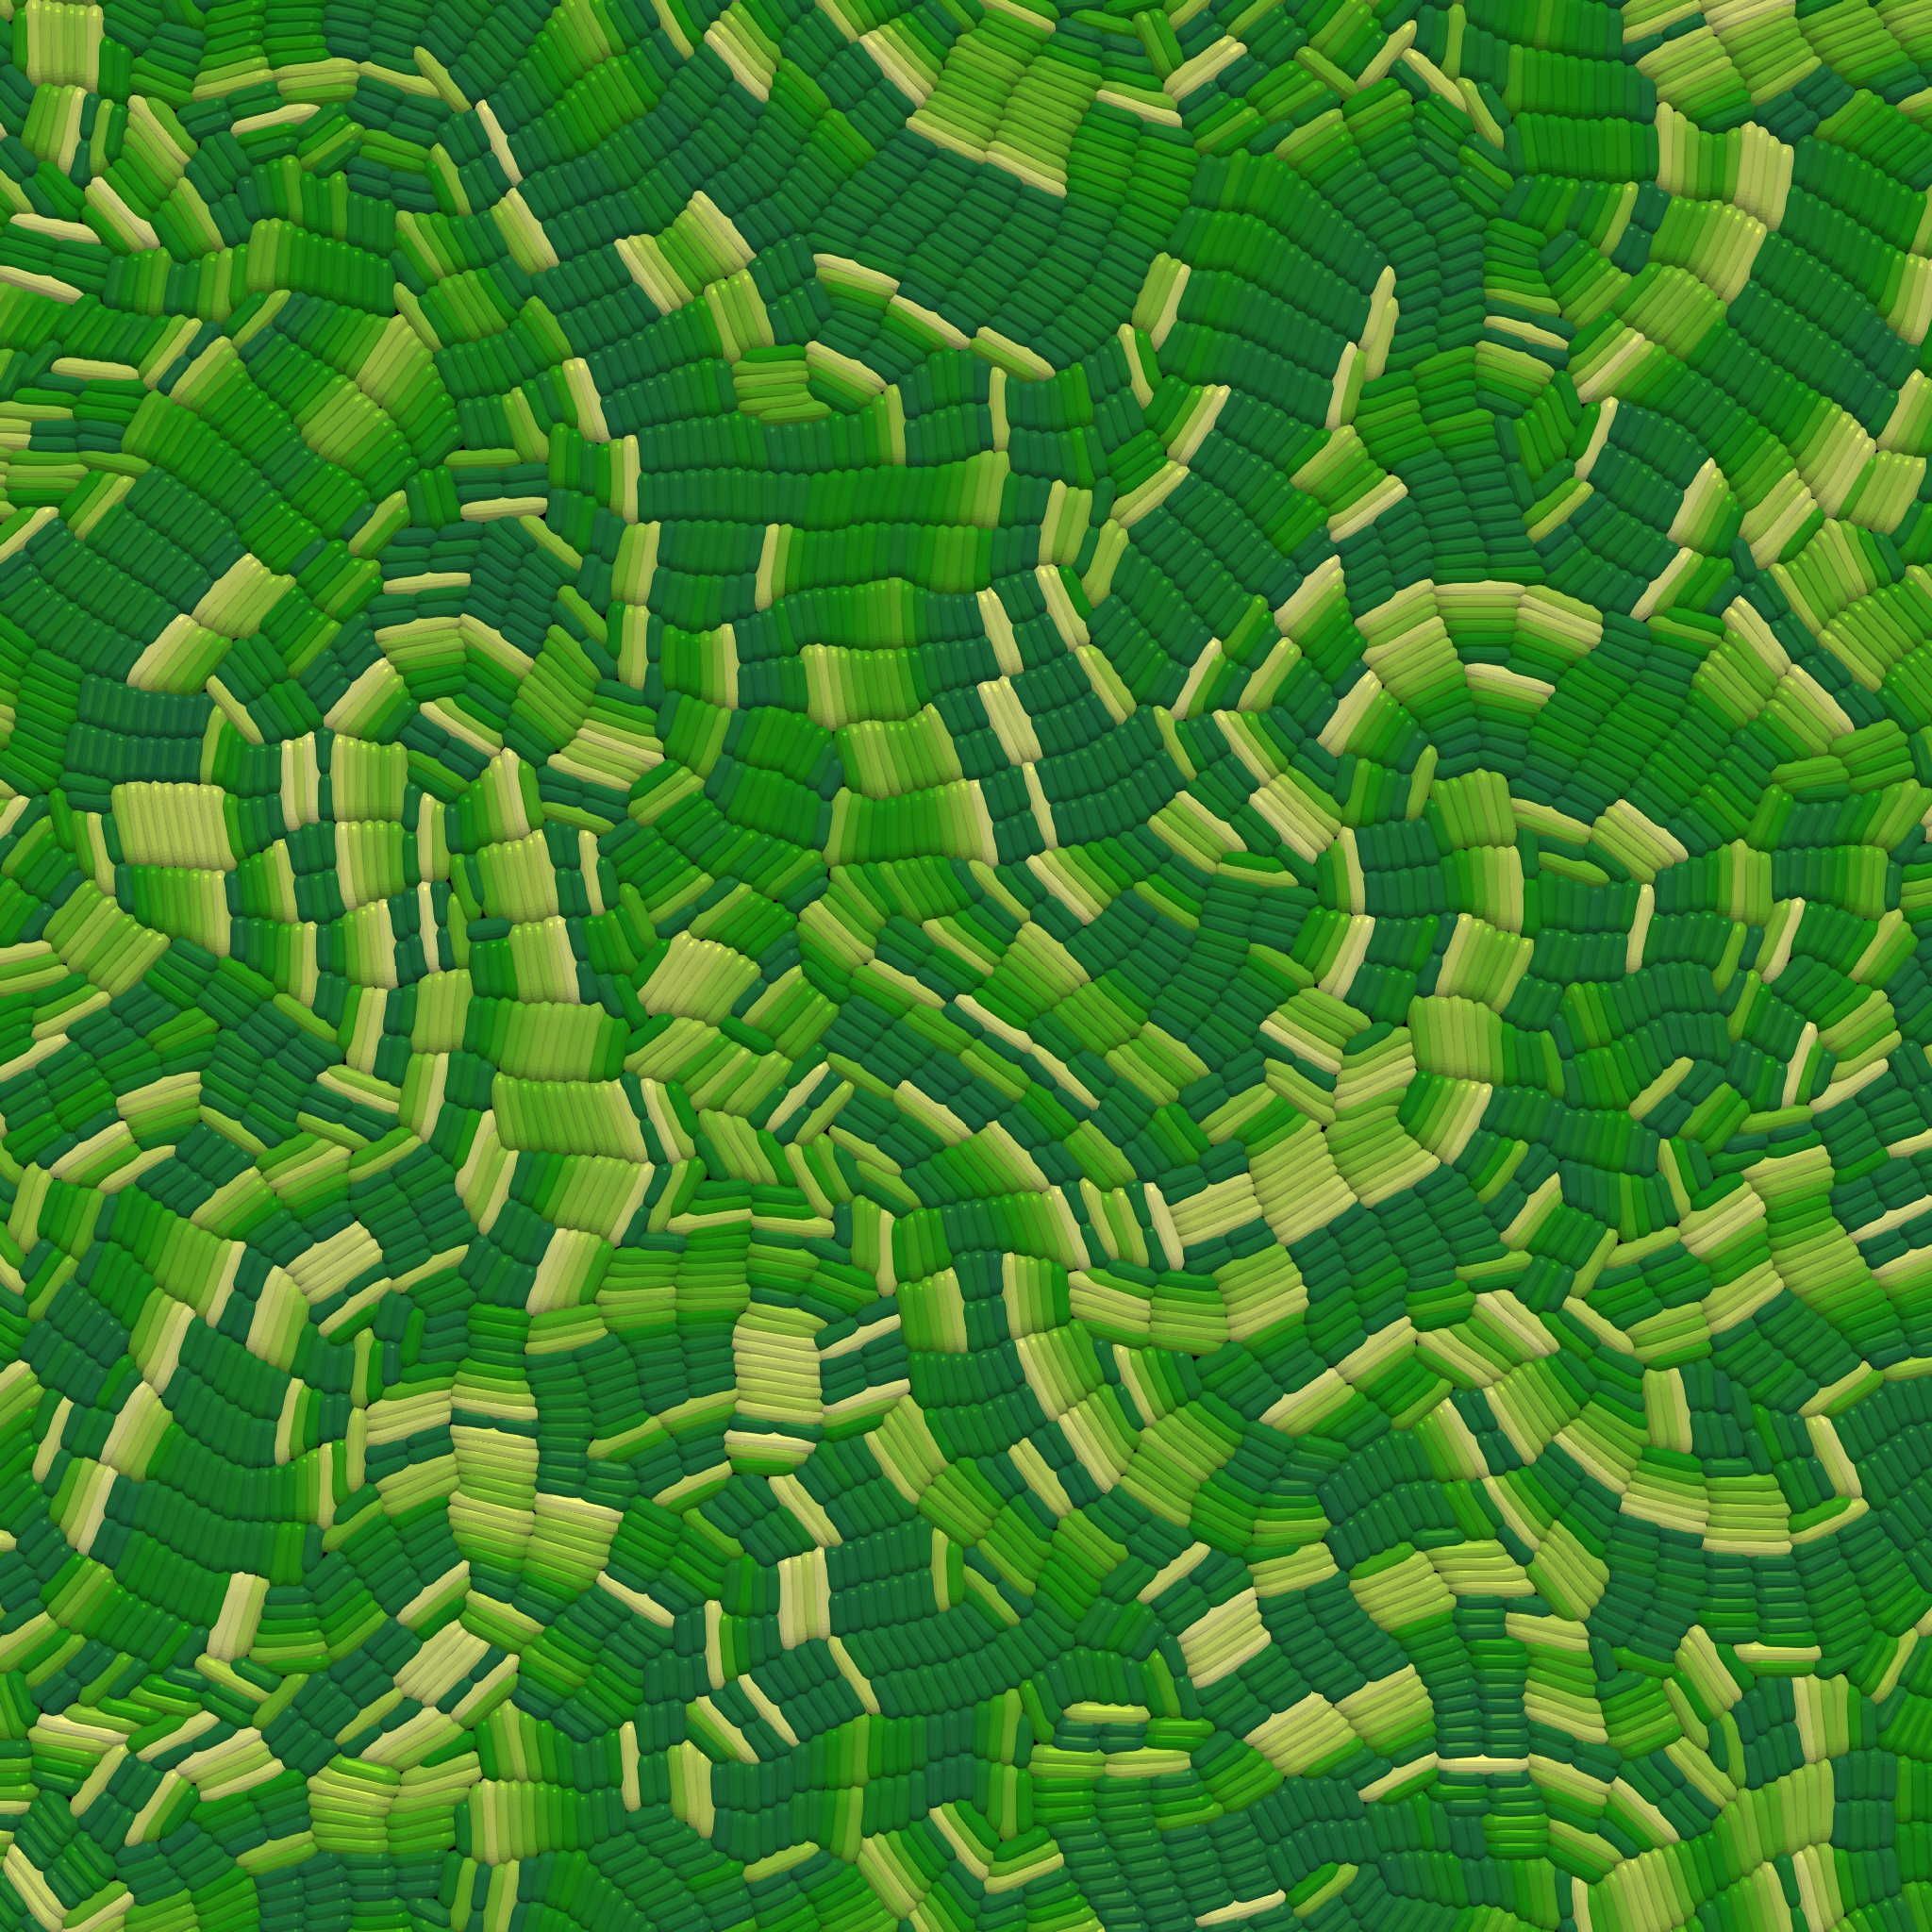
\includegraphics[width=\linewidth]{figures/comparison_plots/density_soft.jpeg}
        \caption{Soft model}
    \end{subfigure}
    \caption{Close-up comparison of cell packing in the colony center for both collision models. The hard model (a) maintains near-optimal packing, while the soft model (b) exhibits significant overlap and overcrowding.}
    \label{fig:dense_packing_comparison}
\end{figure}

\begin{figure}[H]
    \centering
    \begin{subfigure}[b]{\linewidth}
        \centering
        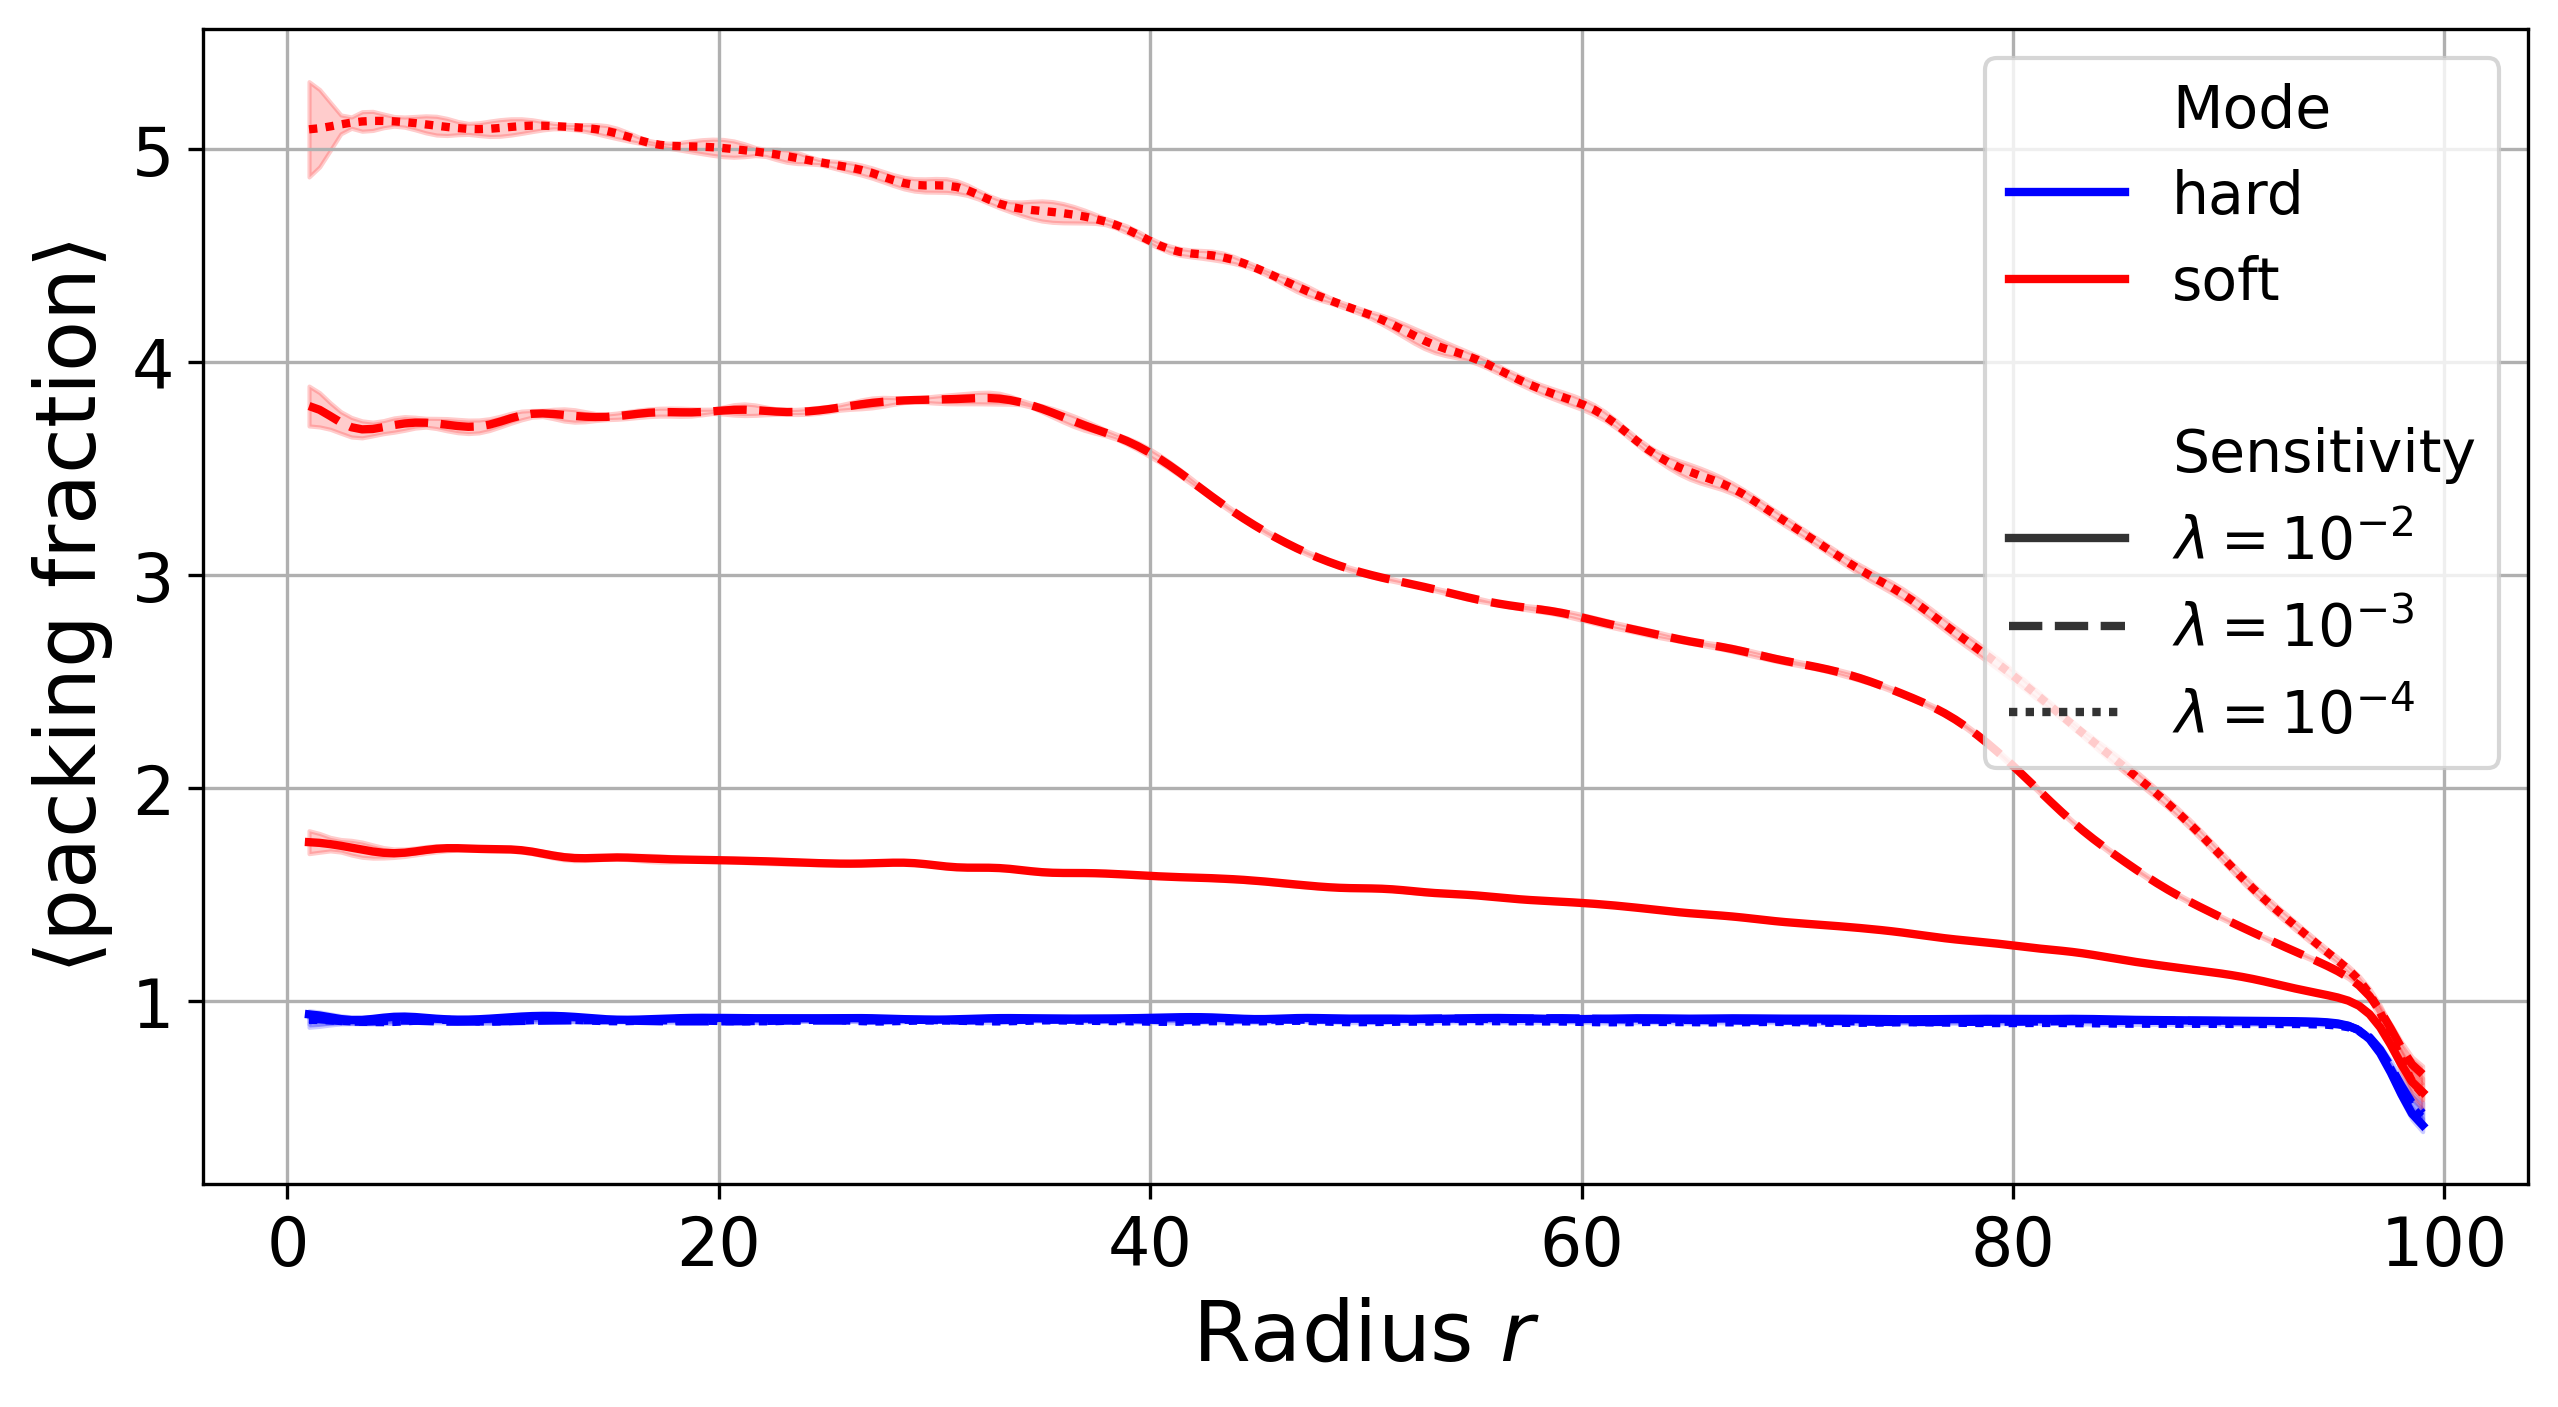
\includegraphics[width=\linewidth]{figures/comparison_plots/combined_radial_packing_fraction.png}
        \caption{Radial packing fraction profiles ($\phi = \frac{A_{\text{cells}}}{A_{\text{total}}}$) for both models. Here $A_{\text{cells}}$ is the total area occupied by cells within a radial bin of width 2 at distance $r$ from the colony center, and $A_{\text{total}}$ is the annular area of that bin. The hard model maintains nearly optimal packing, while the soft model exhibits higher fractions in the colony center.}
        \label{fig:radial_distribution_packing_fraction}
    \end{subfigure}

    \begin{subfigure}[b]{\linewidth}
        \centering
        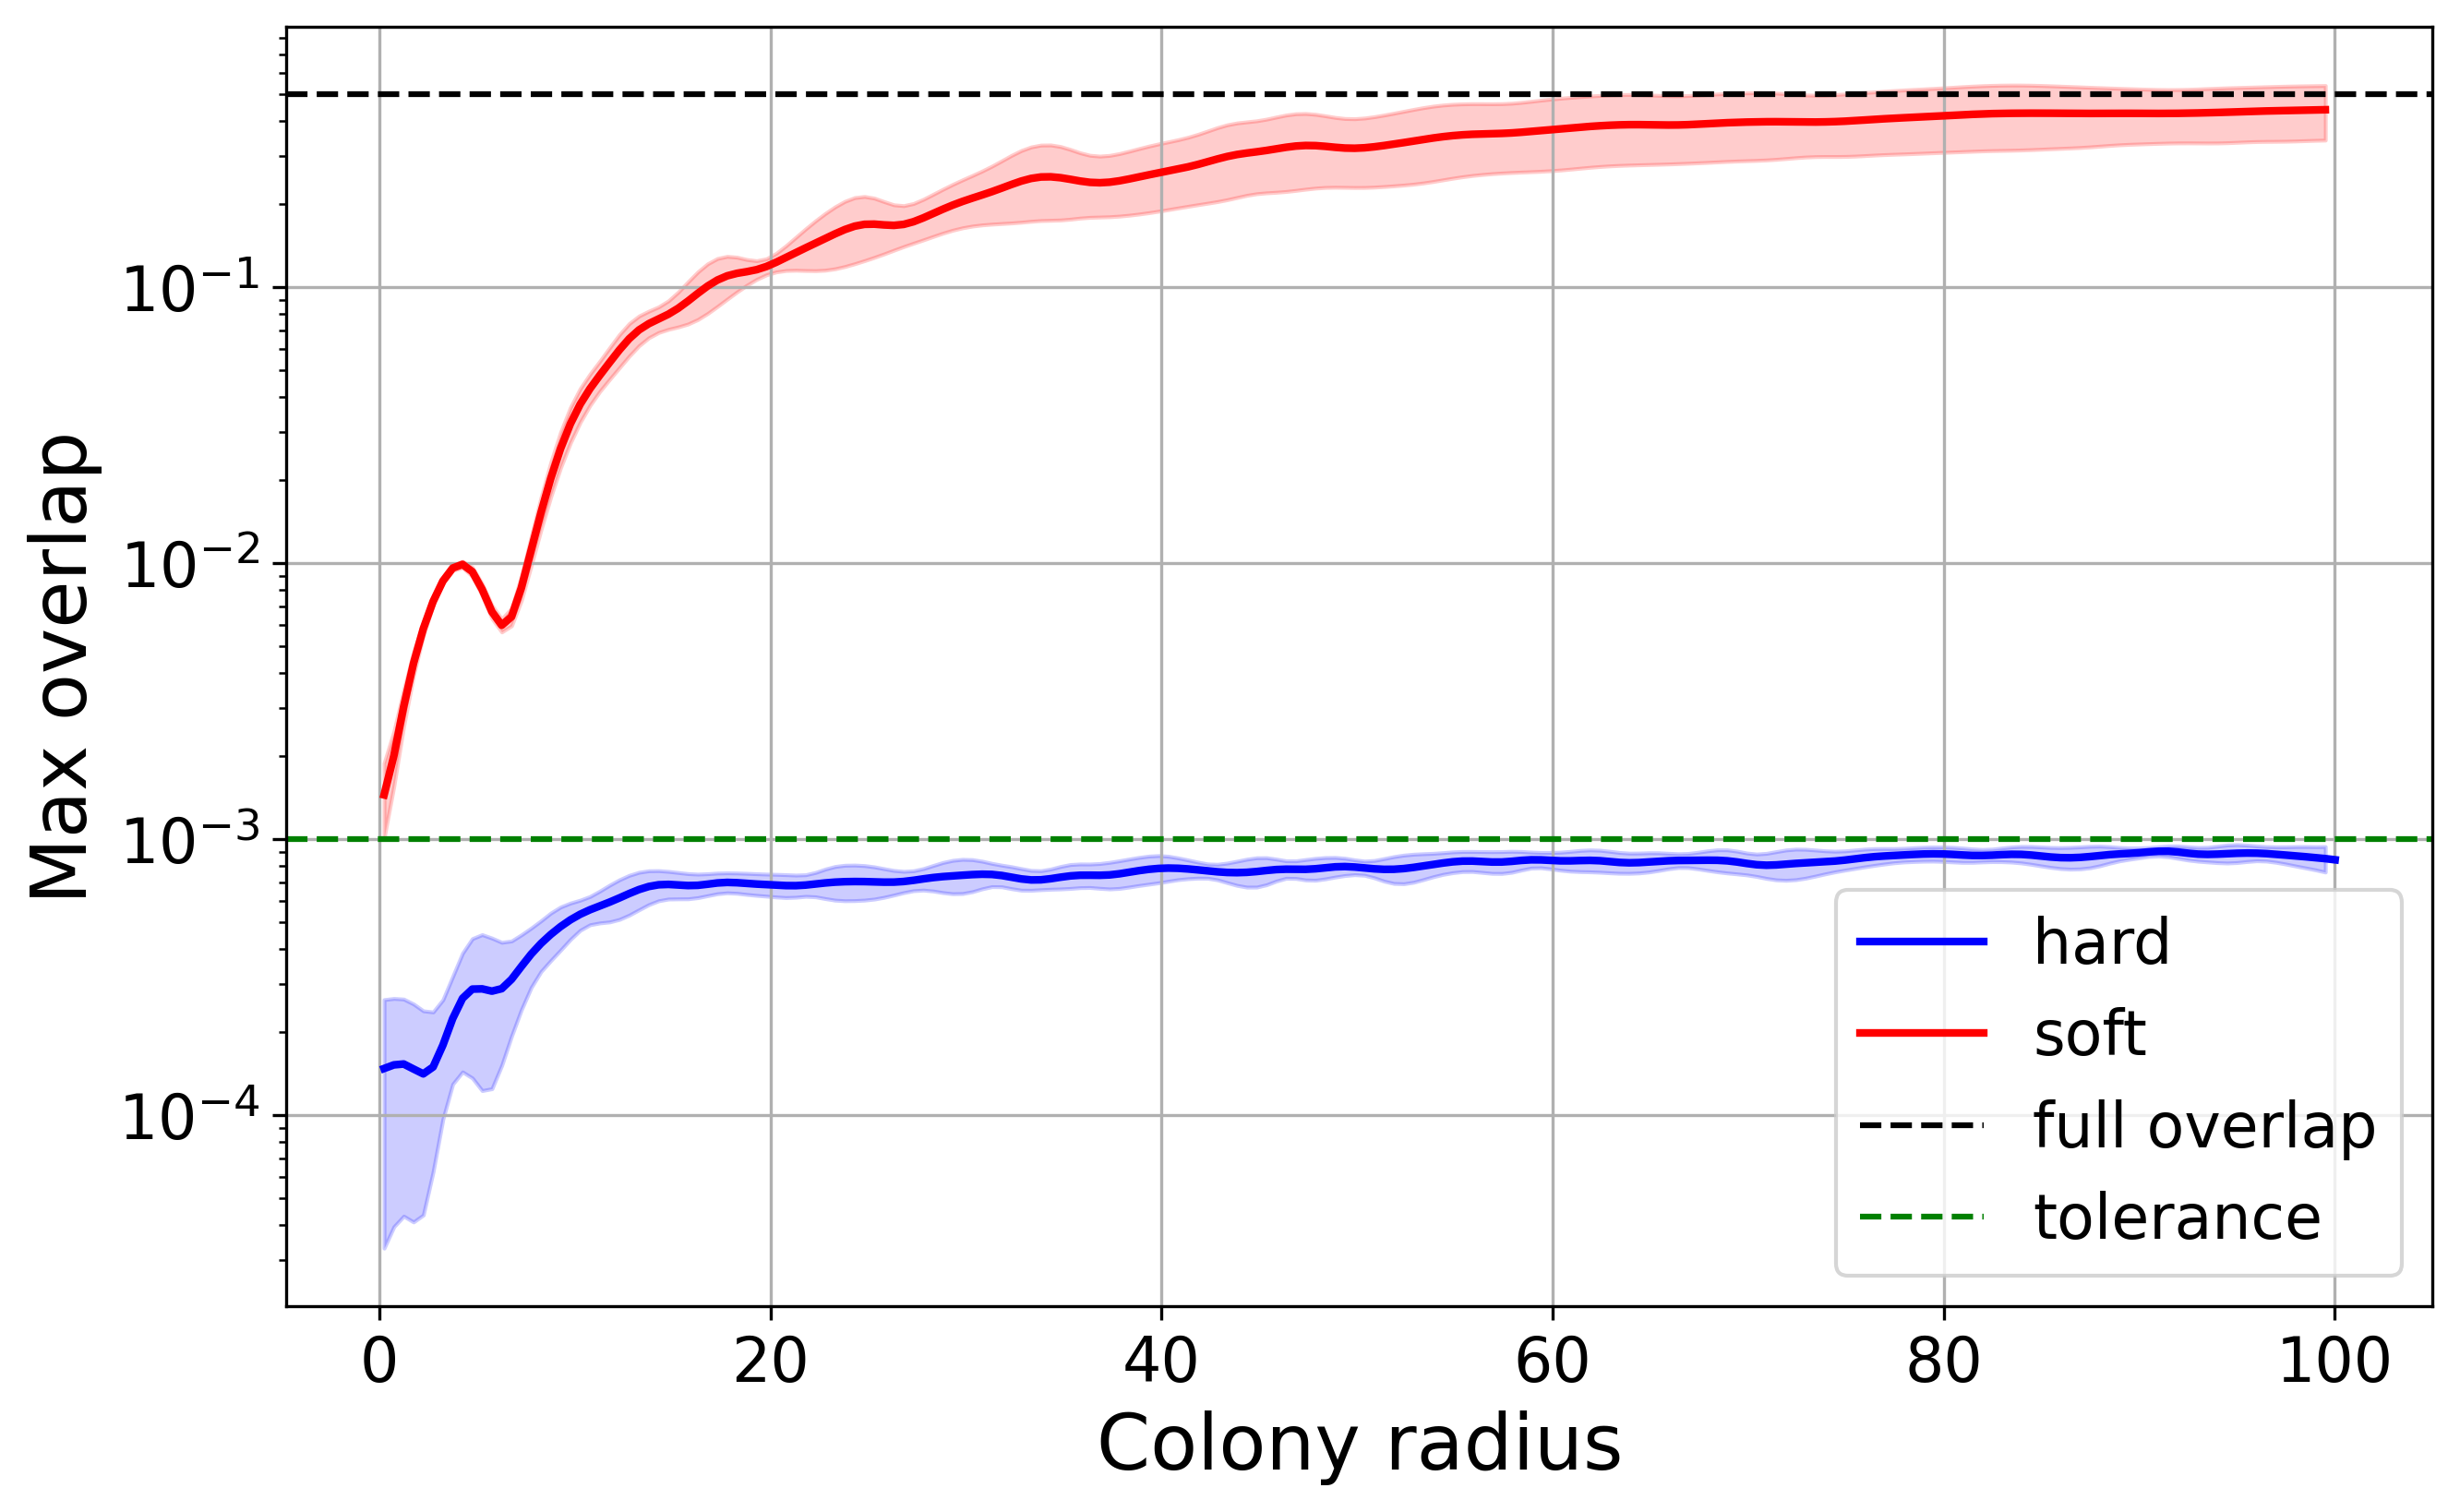
\includegraphics[width=\linewidth]{figures/comparison_plots/combined_colony_radius_vs_max_overlap_with_lines.png}
        \caption{Maximum cell overlap over simulation time. The hard model maintains overlap near the solver tolerance $\epsilon = 10^{-3}$, while the soft model exhibits steady increase, reaching near-complete overlap by the simulation end.}
        \label{fig:max_overlap_simulation}
    \end{subfigure}

    \caption{Cell packing analysis comparing hard and soft collision models.}
    \label{fig:combined_packing_analysis}
\end{figure}

\subsection{Colony Growth Dynamics and Number of Cells}
\label{sec:colony_growth_dynamics}

Despite the severe overcrowding in the soft model, cell packing density does not meaningfully impact colony expansion speed or ring pattern formation (see \autoref{fig:pattern_formation} and \autoref{fig:sim_time_vs_colony_radius}).

However, the soft model requires significantly more cells to reach the same colony radius (see \autoref{fig:colony_radius_vs_num_cells}). At low stress-sensitivity ($\lambda = 10^{-4}$), where growth is largely decoupled from mechanical inhibition, the soft model requires almost three times as many cells as the hard model to reach the same radius. This disparity indicates that the overcrowded interior cannot effectively contribute to outward colony pressure: interior cells remain essentially stationary, while still growing and dividing, leading to a large excess of cells that do not aid expansion.

The computational implications are significant: the soft model must simulate substantially more cells to achieve equivalent colony sizes, directly increasing memory usage and runtime. A detailed performance analysis comparing both models is provided in \autoref{sec:performance_analysis}.

\begin{figure}[h]
    \centering
    \begin{subfigure}[b]{\linewidth}
        \centering
        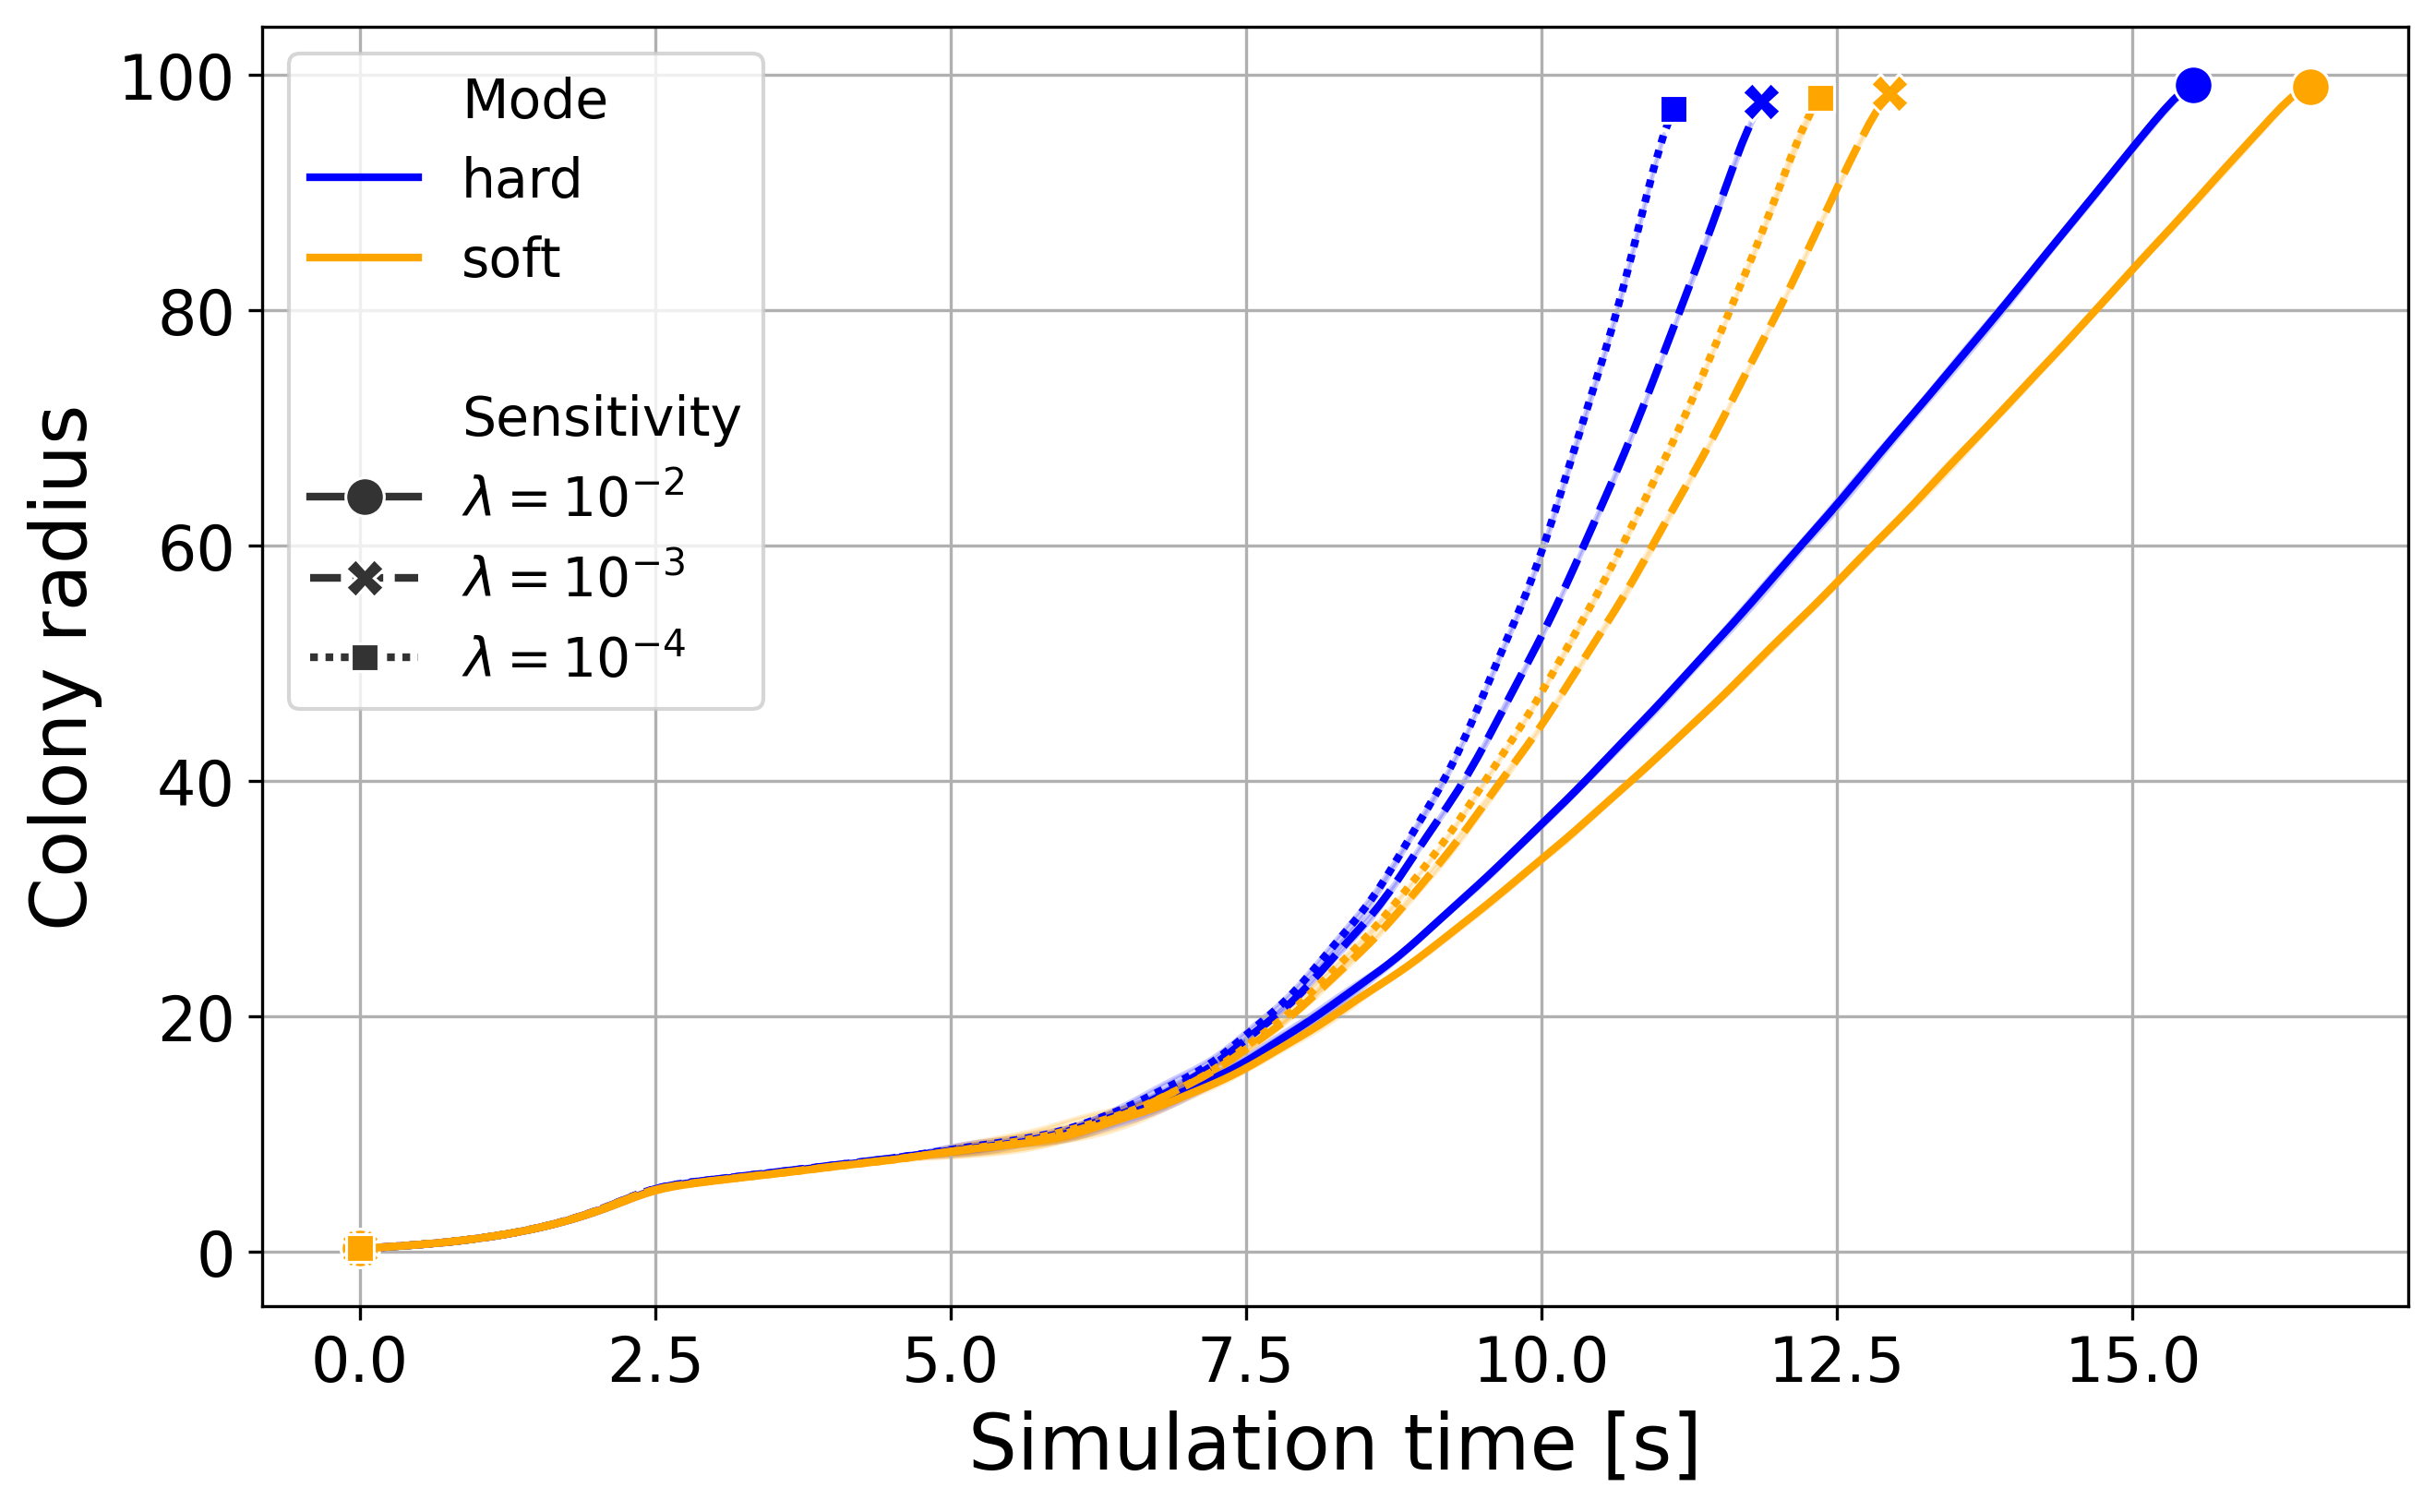
\includegraphics[width=\linewidth]{figures/comparison_plots/combined_simulation_time [s]_vs_colony_radius.png}
        \caption{Simulation time vs. colony radius. Both models exhibit similar growth dynamics, though the soft model is slightly slower due to allowable cell overlap.}
        \label{fig:sim_time_vs_colony_radius}
    \end{subfigure}

    \begin{subfigure}[b]{\linewidth}
        \centering
        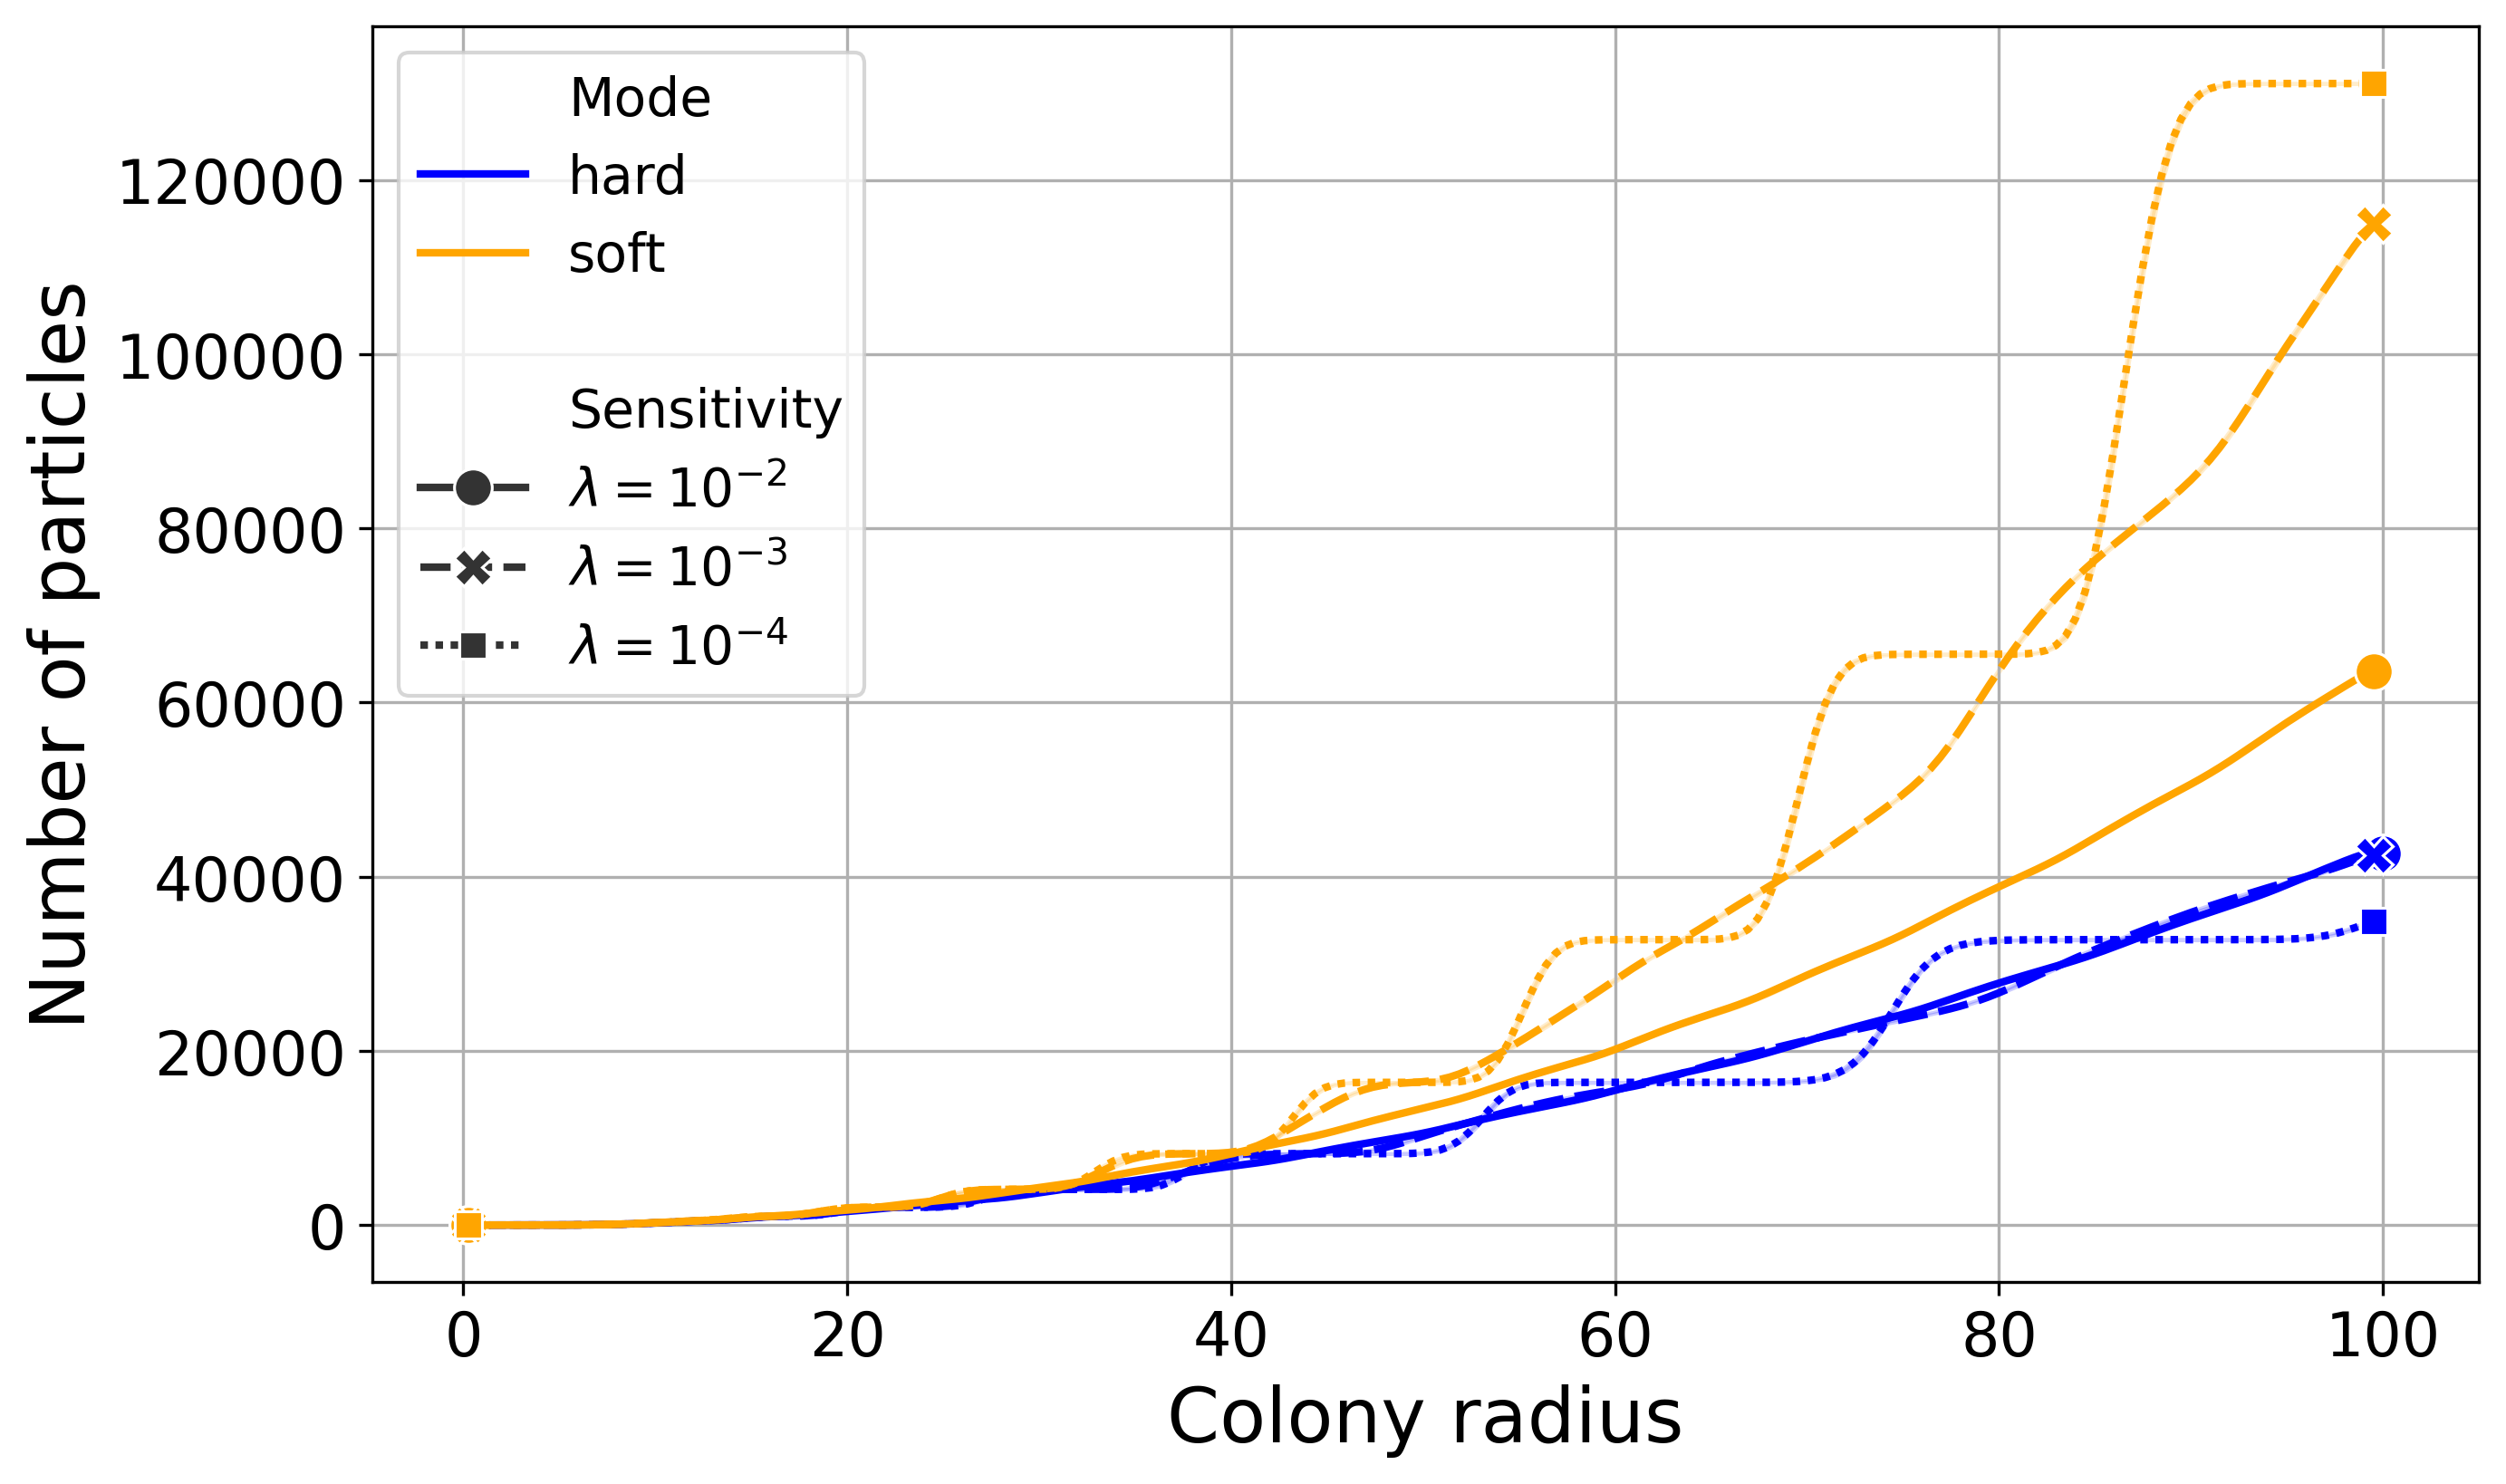
\includegraphics[width=\linewidth]{figures/comparison_plots/combined_colony_radius_vs_num_particles.png}
        \caption{Number of cells required to reach a given colony radius. The soft model requires substantially more cells, particularly at low stress-sensitivity ($\lambda = 10^{-4}$).}
        \label{fig:colony_radius_vs_num_cells}
    \end{subfigure}

    \caption{Colony growth dynamics and cell scaling comparison between hard and soft models.}
    \label{fig:comparison_combined}
\end{figure}

\subsection{Microdomain Formation}
\label{sec:microdomain_formation}

Similar to You et al.~\cite{You2018,You_2021}, we observe the formation of microdomains, defined as localized regions where cells share similar orientations. These domains emerge from mechanical interactions and growth dynamics. As shown in \autoref{fig:orientation_comparison_small}, both hard and soft collision models reproduce this phenomenon for small colonies ($R \approx 50$), producing patterns that closely resemble experimental observations of real \textit{E. coli} colonies~\cite{You2018}.

\begin{figure}[H]
    \centering
    \begin{subfigure}[b]{0.49\columnwidth}
        \centering
        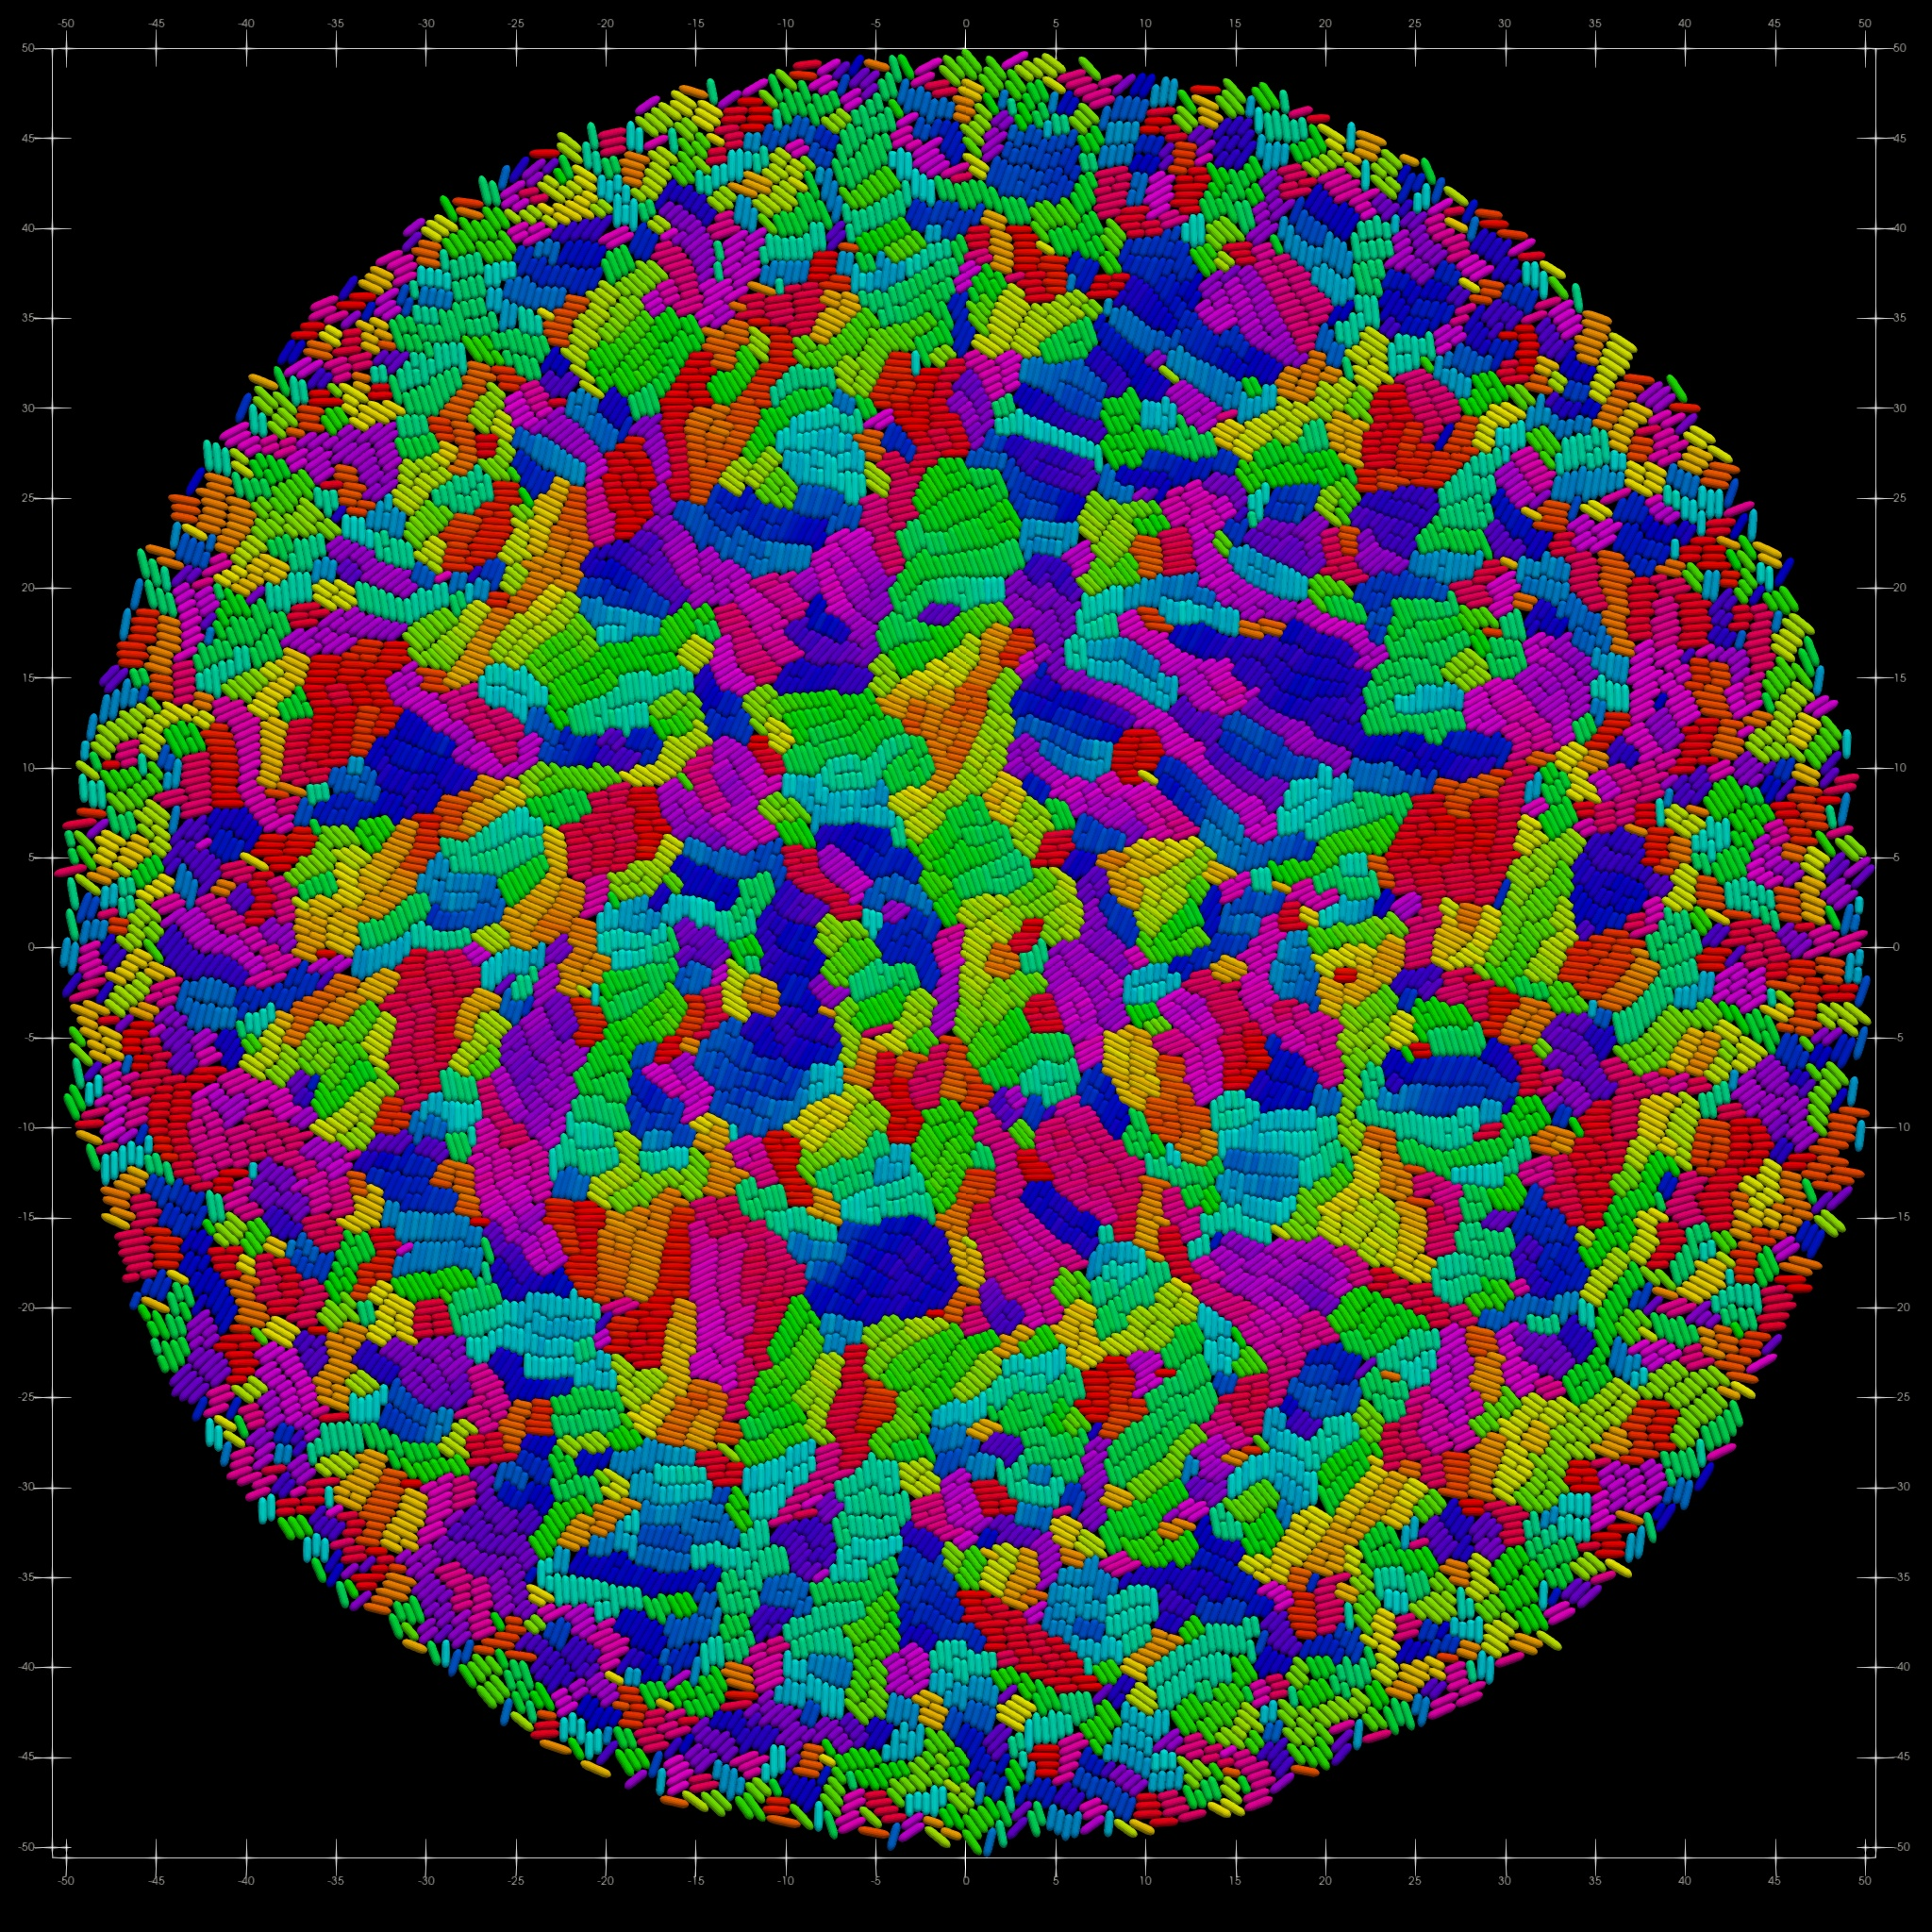
\includegraphics[width=\linewidth]{figures/orientation_comparisons/r50_soft_e-2.jpeg}
        \caption{Soft model at $R \approx 50$.}
    \end{subfigure}
    \begin{subfigure}[b]{0.49\columnwidth}
        \centering
        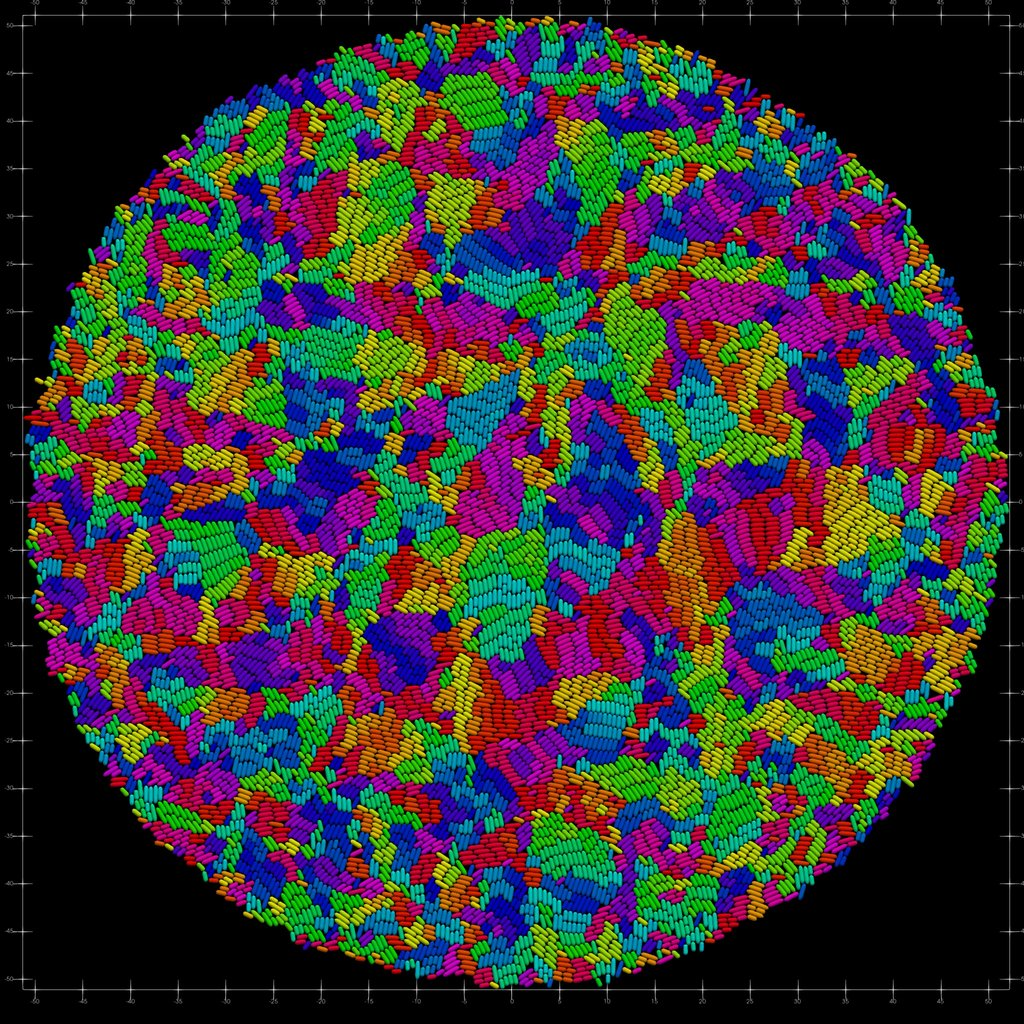
\includegraphics[width=\linewidth]{figures/orientation_comparisons/r50_hard_e-2.jpeg}
        \caption{Hard model at $R \approx 50$.}
    \end{subfigure}
    \caption{Cell orientation patterns for both models. Color indicates cell orientation angle.}
    \label{fig:orientation_comparison_small}
\end{figure}

Even though the hard and soft collision models presented in this paper are not directly comparable to You et al.~\cite{You2018}, as You et al. use constant growth rates while the models here employ stress-dependent growth, their observations still provide useful context. You et al. showed that reduced growth rates produce larger microdomains. In the models presented here, stress sensitivity $\lambda$ mimics this effect by inhibiting growth in the densely packed colony center, which similarly produces larger microdomains. We observe this trend in simulations of the soft model (see \autoref{fig:orientation_comparison}), where higher $\lambda$ values lead to reduced growth rates and correspondingly larger microdomains, consistent with You et al.'s findings. The hard model shows no such trend.

\subsection{Microdomain Formation in Large Colonies}

Although the hard and soft models produce similar orientation patterns in small colonies ($R \approx 50$), pronounced differences emerge as colonies grow larger or $\lambda$ decreases. As shown in \autoref{fig:orientation_comparison}, the hard model maintains distinct patches of similarly-sized aligned cells across all $\lambda$ values. In contrast, the soft model produces elongated, unrealistic bundles of densely packed aligned cells that do not resemble experimentally observed microdomains.

This artifact stems directly from the soft model's higher interior growth rates, which cannot be effectively resolved by local pairwise repulsive forces. Without sufficient outward stress propagation, the interior becomes unphysically dense, forcing cells into long, aligned bundles.

The impact of $\lambda$ on microdomain structure is clearly visible: the hard model consistently produces microdomains of similar area across all stress-sensitivity values, while the soft model exhibits a broad distribution with many large clusters, particularly at low $\lambda = 10^{-4}$ (see Figure~\ref{fig:cluster_area_boxplot}).

\begin{figure}[h]
    \centering
    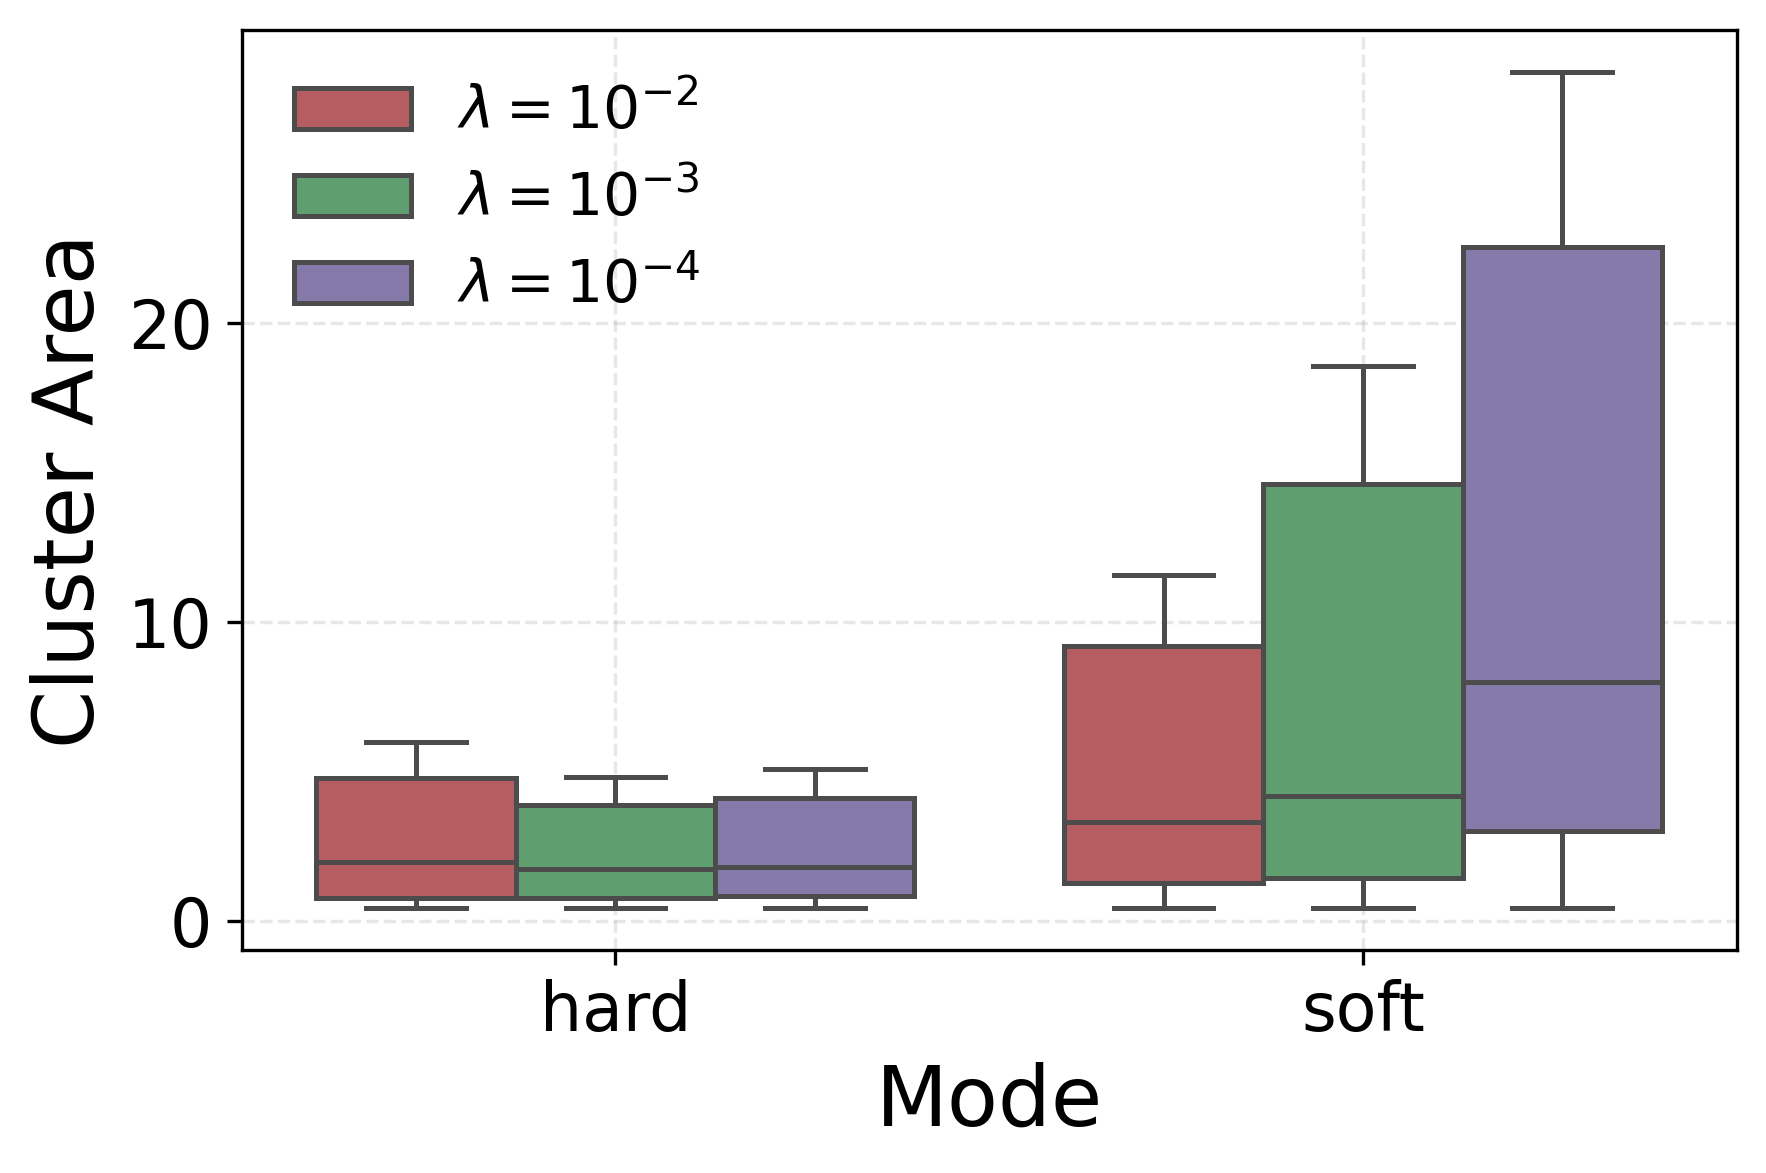
\includegraphics[width=\linewidth]{figures/comparison_plots/cluster_area_boxplot.png}
    \caption{Microdomain area distributions for large colonies ($R \approx 100$) across $\lambda$ values. The hard model produces consistent domain sizes, while the soft model shows high variability with many large clusters, especially at $\lambda = 10^{-4}$. Clusters are identified using connected-component labeling~\cite{You2018}, grouping neighboring cells with similar orientations.}
    \label{fig:cluster_area_boxplot}
\end{figure}

\subsection{Implications for Model Selection}

Both models successfully reproduce microdomain formation in small colonies ($R \lesssim 50$), demonstrating that the fundamental mechanisms are captured adequately by both collision approaches at small scales. However, substantial differences emerge as colonies grow larger or $\lambda$ decreases. The soft model's unphysical packing density progressively distorts domain structure, producing elongated cell bundles that do not match experimental observations. In contrast, the hard model maintains biologically realistic domain morphologies across all tested parameters.

Potential improvements to the soft model could address these limitations. An enhanced adaptive timestep scheme could reduce $\Delta t$ when packing fraction exceeds a threshold, allowing repulsive forces more time to resolve overlaps before they accumulate. Additionally, introducing a global outward pressure or expansion force could help prevent excessive interior packing by providing a uniform resistance to overcrowding, distributing mechanical stress more effectively throughout the colony.

In its current form, the soft model is unsuitable for studying microdomain formation in large colonies or at low stress-sensitivity. However, it remains a viable and computationally simpler alternative for studying macroscopic pattern formation in smaller colonies where packing artifacts do not significantly distort the overall dynamics, such as those explored in~\cite{You2018}. For studies requiring accurate microdomain resolution or exploration of parameter regimes with weak stress-sensitivity, the hard model is the appropriate choice.

\begin{figure*}[p]
    \makebox[\textwidth][c]{
        \centering

        \begin{tabular}{r M{0.36\textwidth} M{0.36\textwidth} }
             & Hard Model & Soft Model \\
            \orientationcomparisonrow{$\lambda=10^{-2}$}{-2}
            \orientationcomparisonrow{$\lambda=10^{-3}$}{-3}
            \orientationcomparisonrow{$\lambda=10^{-4}$}{-4}
        \end{tabular}
    }

    \caption{Comparison of orientation patterns at different stress sensitivities in the center of the colony. The color indicates the cells orientation, with similar colors representing similar angles. The hard model is able to maintain visible patches of aligned cells for all stress sensitivities, whereas the soft model tends to produce long bundles of densely packed cells for low stress sensitivies. This effect is caused by a lack of seperation forces causing cells in the center of the colony to pile up.}
    \label{fig:orientation_comparison}
\end{figure*}

\subsection{Radial Stress Distribution and Growth Rate}

Another key difference between the two modeling approaches lies in the radial stress distribution that develops within the colony (see \autoref{fig:radial_distribution_stress}). Both the hard and soft models produce qualitatively similar radially averaged stress profiles, consistent with the behavior originally reported in~\cite{Weady2024}. In both cases, the stresses are highest at the colony center and gradually decrease toward the outer edge, reflecting the buildup of mechanical compression in the densely packed interior. These profiles approximately follow the derived analytical expression $p(r) \approx \frac{2}{\lambda} \ln\left(\frac{1}{8 c} - c\lambda r^2 \right)$, which predicts a logarithmic dependence on the colony radius.

Although the overall shape of the profiles is comparable, the magnitude of the predicted stresses differs substantially between the two models. Quantitatively, the hard model produces stress values that are approximately 1.5 times higher than the analytical prediction, whereas the soft model yields stresses that are only about half the analytical value. This two-fold variation in stress magnitude is significant and likely plays a central role in explaining the discrepancies in growth dynamics and microdomain organization discussed in \autoref{sec:colony_growth_dynamics} and \autoref{sec:microdomain_formation}.

\begin{figure*}[b]
    \centering
    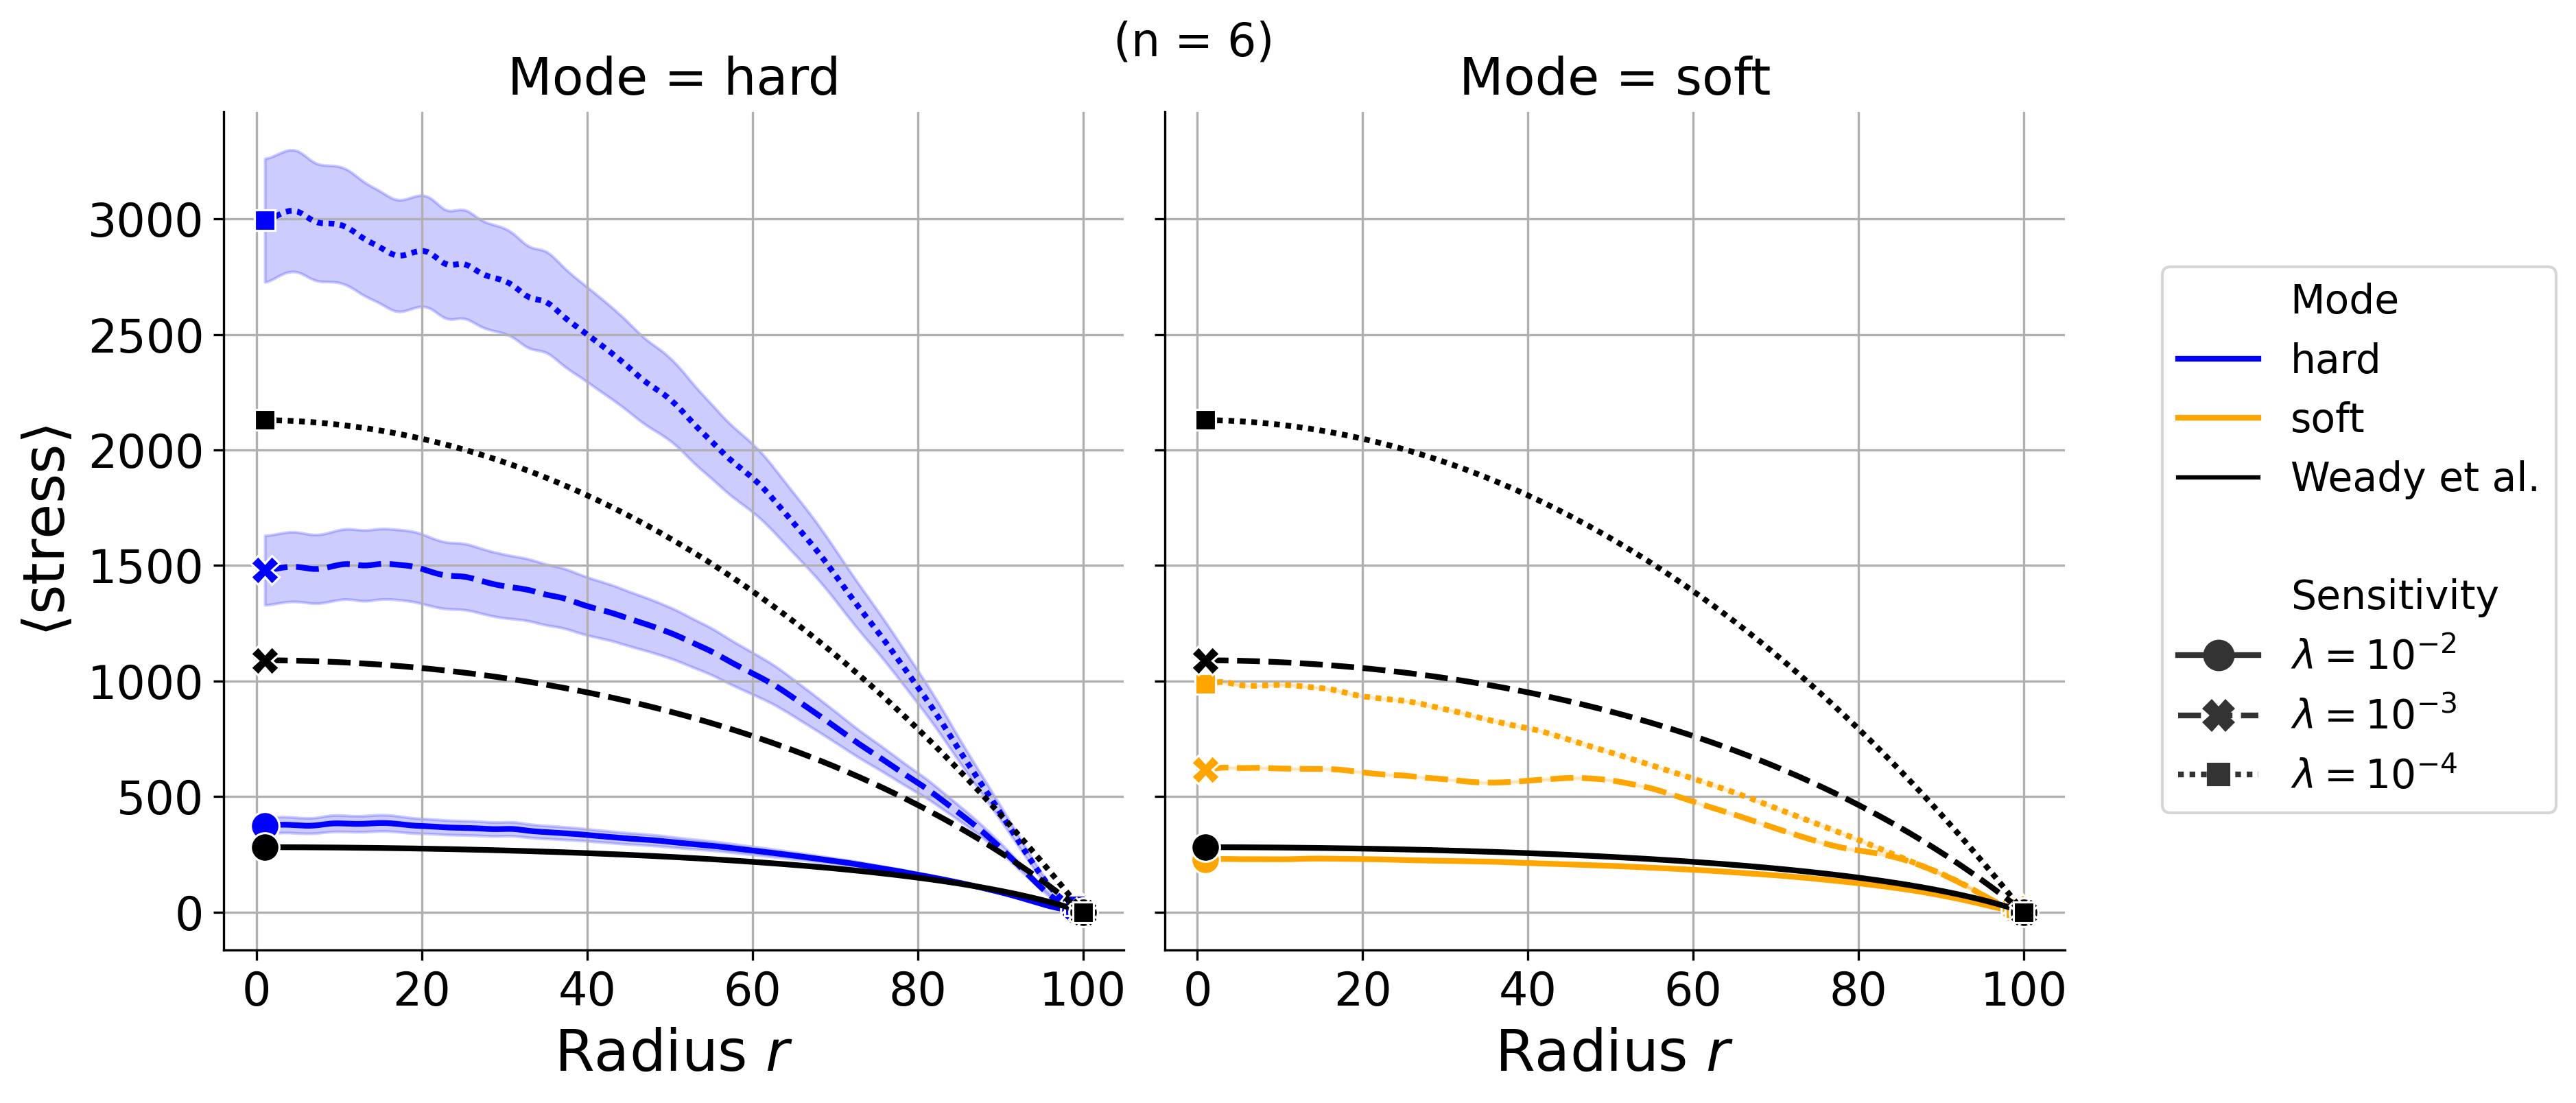
\includegraphics[width=\linewidth]{figures/comparison_plots/combined_stress_shared.png}
    \caption{Radial stress profiles for both models across different $\lambda$ values. Both models produce similar qualitative stress distributions, with stresses highest in the colony center and decreasing toward the edge following the analytical profile. However, the hard model consistently predicts higher stresses, while the soft model predicts lower stresses.}
    \label{fig:radial_distribution_stress}
\end{figure*}

The consistently elevated stresses observed in the hard model, as also noted by Weady et al.~\cite{Weady2024}, are likely a consequence of the discrete cell-based representation not fully satisfying the continuum assumptions used in the analytical derivation. In contrast, the soft model produces lower stresses because it lacks a global force propagation mechanism: stress is transmitted only through local pairwise repulsive interactions, which are insufficient to communicate mechanical load effectively across the entire colony. Consequently, stresses in the colony interior remain low, and central cells experience weaker mechanical inhibition. These cells therefore continue to grow and divide, eventually leading to the overcrowding and distorted microdomain patterns described in \autoref{sec:colony_growth_dynamics}.

The consequences of this imbalance in stress transmission are clearly reflected in the radial growth rate profiles. As shown in \autoref{fig:radial_distribution_growth_rate}, cells in the soft model exhibit substantially higher growth rates than those in the hard model throughout most of the colony interior, especially at low stress-sensitivity values ($\lambda = 10^{-3}$ and $\lambda = 10^{-4}$).

At higher stress-sensitivity ($\lambda = 10^{-2}$), growth becomes strongly suppressed in the interior for both models, and only cells near the colony periphery remain actively dividing. This shift from interior-driven to edge-driven proliferation is also apparent in \autoref{fig:sim_time_vs_colony_radius} and is consistent with experimental observations in real microbial systems, including bacterial and yeast colonies such as \textit{E. coli} and \textit{Saccharomyces cerevisiae}~\cite{Warren2019,Hallatschek2007,Giometto2018}.

\begin{figure}[H]
    \centering
    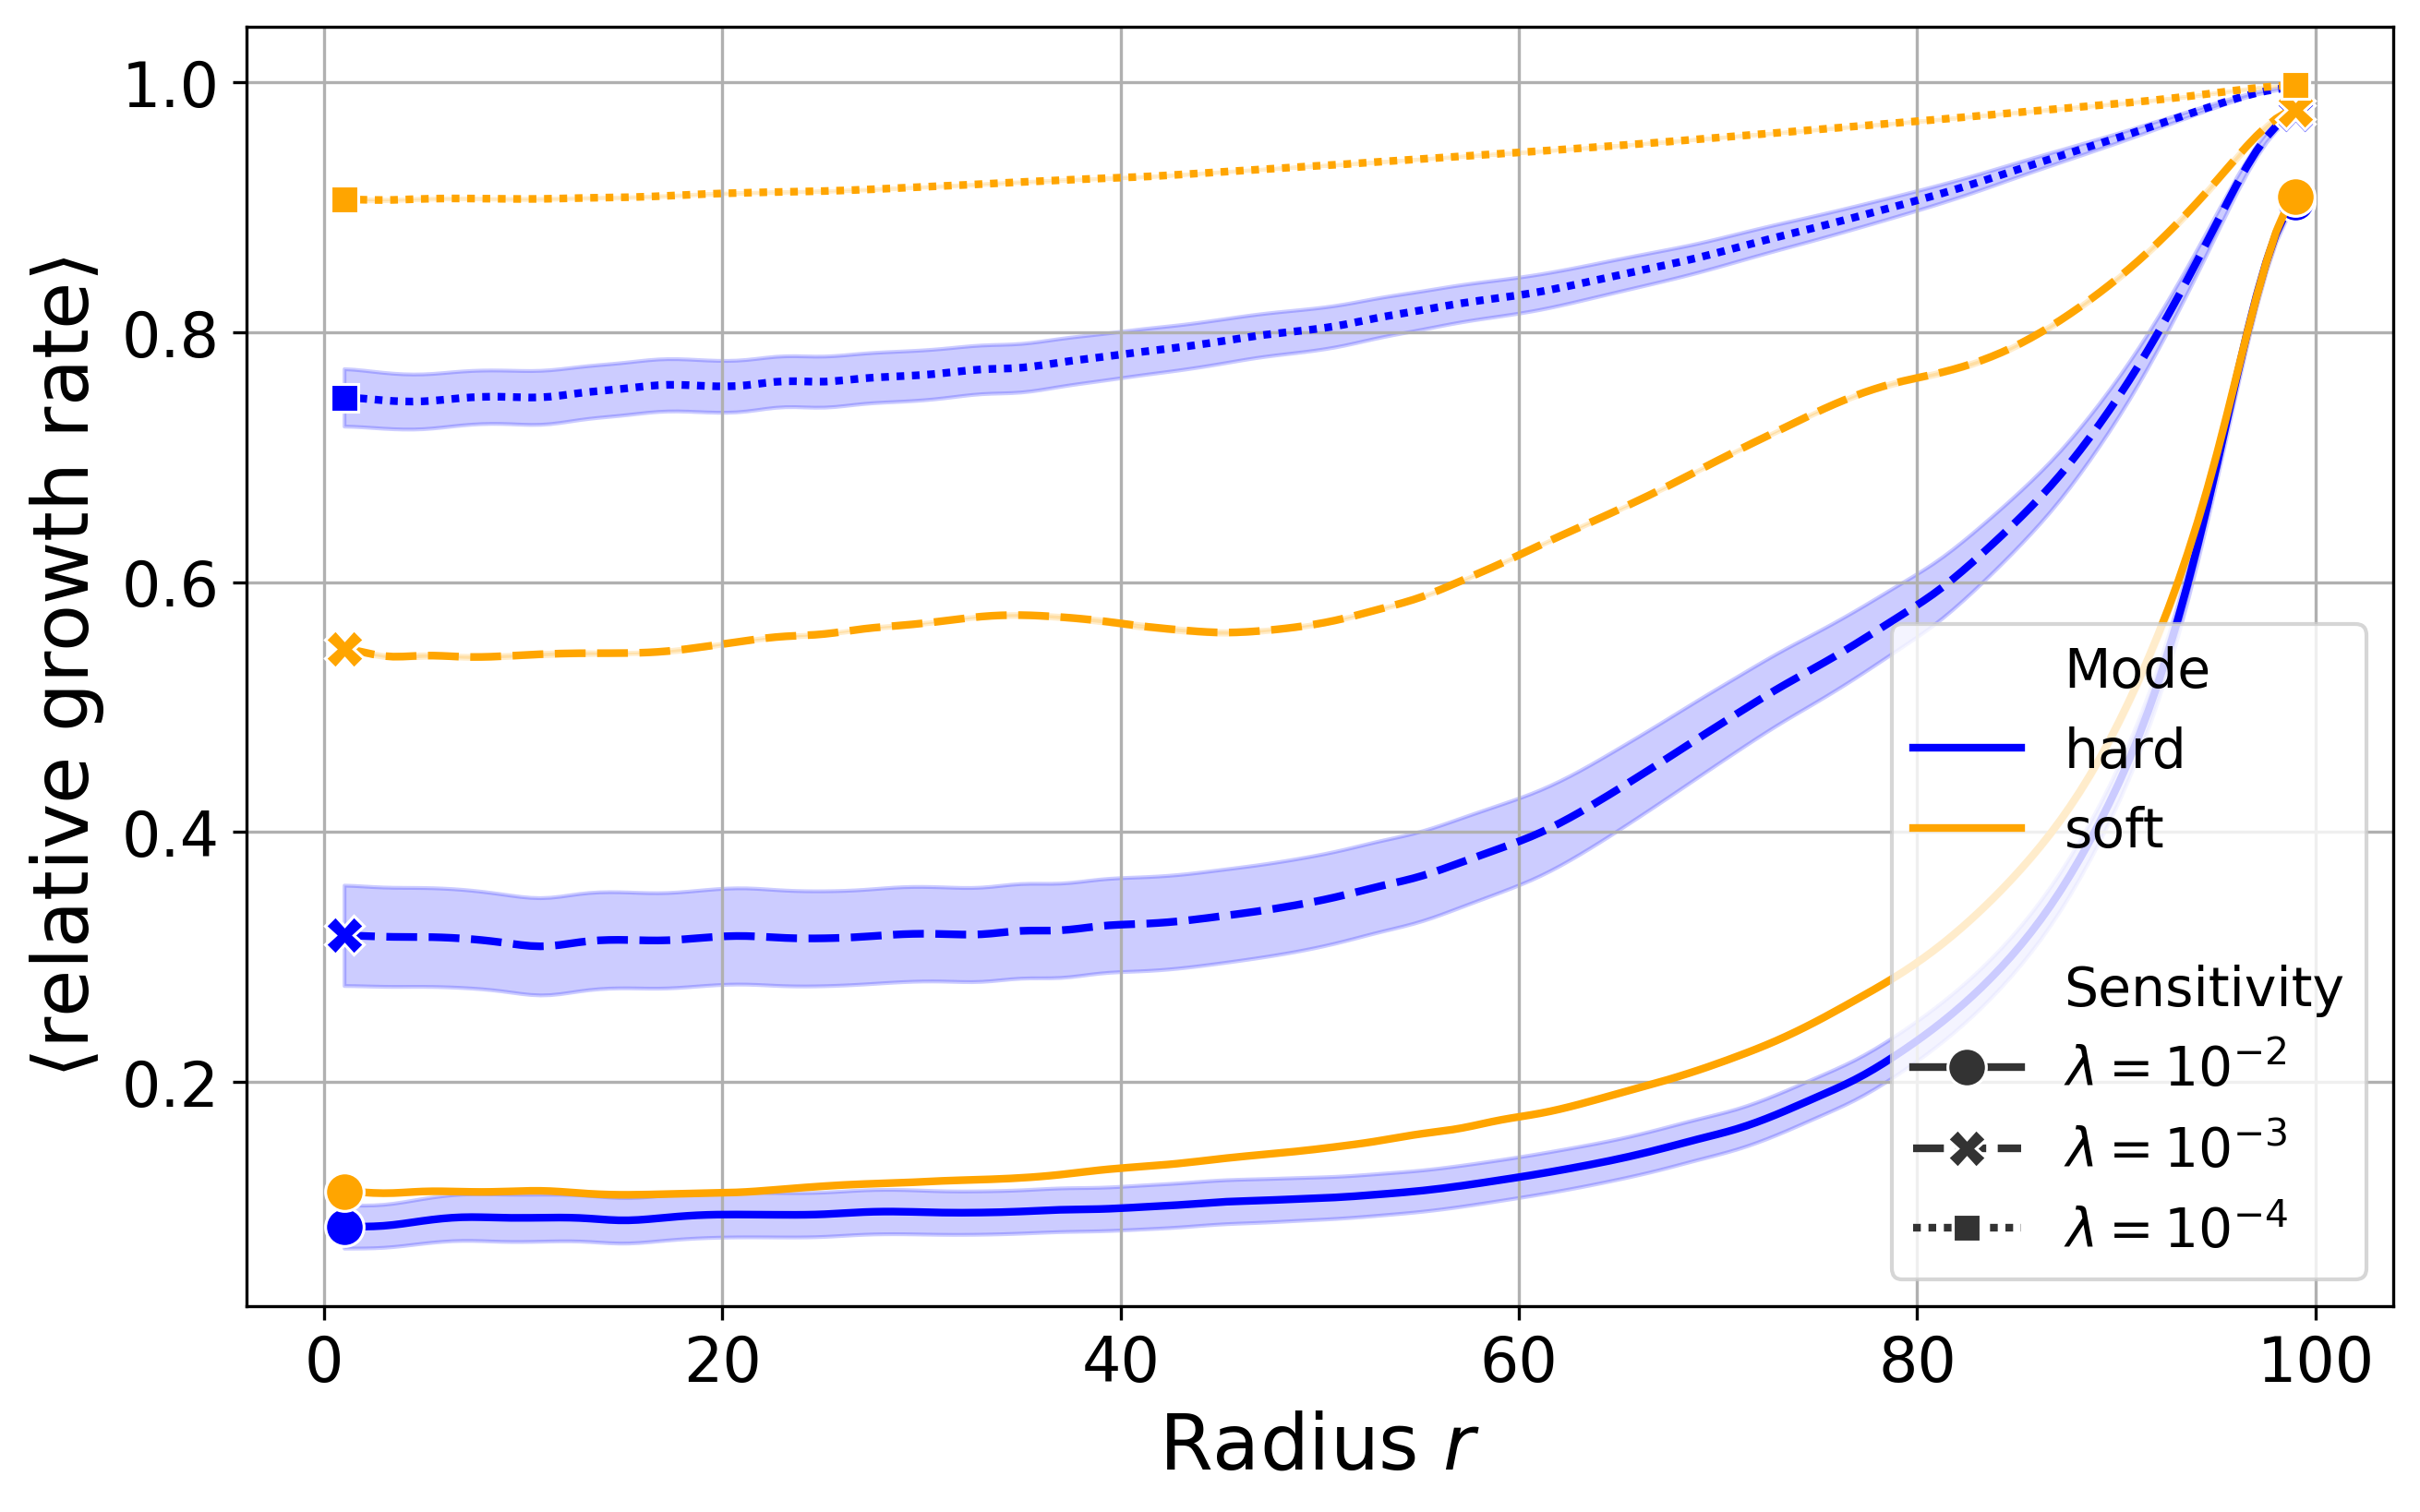
\includegraphics[width=\linewidth]{figures/comparison_plots/combined_radial_impedance.png}
    \caption{Radial relative growth rate profiles ($e^{-\lambda \sigma}$) for both models. Cells in the soft model grow significantly faster than those in the hard model across most of the colony, particularly at low stress-sensitivity ($\lambda = 10^{-3}$ and $\lambda = 10^{-4}$). At high stress-sensitivity ($\lambda = 10^{-2}$), growth is strongly suppressed in the interior of both models, with only cells at the colony edge actively dividing.}
    \label{fig:radial_distribution_growth_rate}
\end{figure}

\section{Computational Performance}
\label{sec:performance_analysis}

Both the hard and soft collision models are capable of reproducing the experimentally observed macroscopic patterns in growing bacterial colonies, including concentric rings and microdomain formation in small colonies. However, they differ significantly in terms of computational performance, which is critical for large-scale simulations. In this section, we analyze and compare the performance of both models in detail.


\subsection{Critical Time Step}

The soft collision model is cheaper per interaction but typically requires smaller integration time steps to maintain numerical stability due to the stiffness of the repulsive forces. In contrast, the hard collision model can often operate with larger time steps since it enforces non-overlap constraints directly, although its per-step cost is significantly higher because of the global optimization problem.

\autoref{fig:simulation_time_vs_dt} shows the maximum stable time step $\Delta t$ for both models during a simulation. The optimal time is determined by \autoref{alg:adaptive_dt}, which adjusts $\Delta t$ based on the median cell velocity to ensure stability. The hard collision model stabilizes around ${\Delta t}_{\text{hard}} \approx 3 \cdot 10^{-4} h$, while the soft model steadily decreases, reaching ${\Delta t}_{\text{soft}} \approx 1 \cdot 10^{-5} h$ at the end. The ratio ${\Delta t}_{\text{hard}}/{\Delta t}_{\text{soft}} \approx 30$ indicates that the hard model can take roughly 30 times larger steps than the soft model in dense colonies, and thus requires significantly fewer steps to simulate the same physical time span.

Interestingly, for the hard model with $\lambda=10^{-2}$, the maximum stable time step increases over time. This occurs because cells in the colony interior stop growing (see \autoref{fig:radial_distribution_growth_rate}), reducing the median particle velocity $u_m$ and allowing larger steps. The soft model does not exhibit this effect, as repulsive forces always permit some overlap and sporadic motion.

\begin{figure}[H]
    \centering
    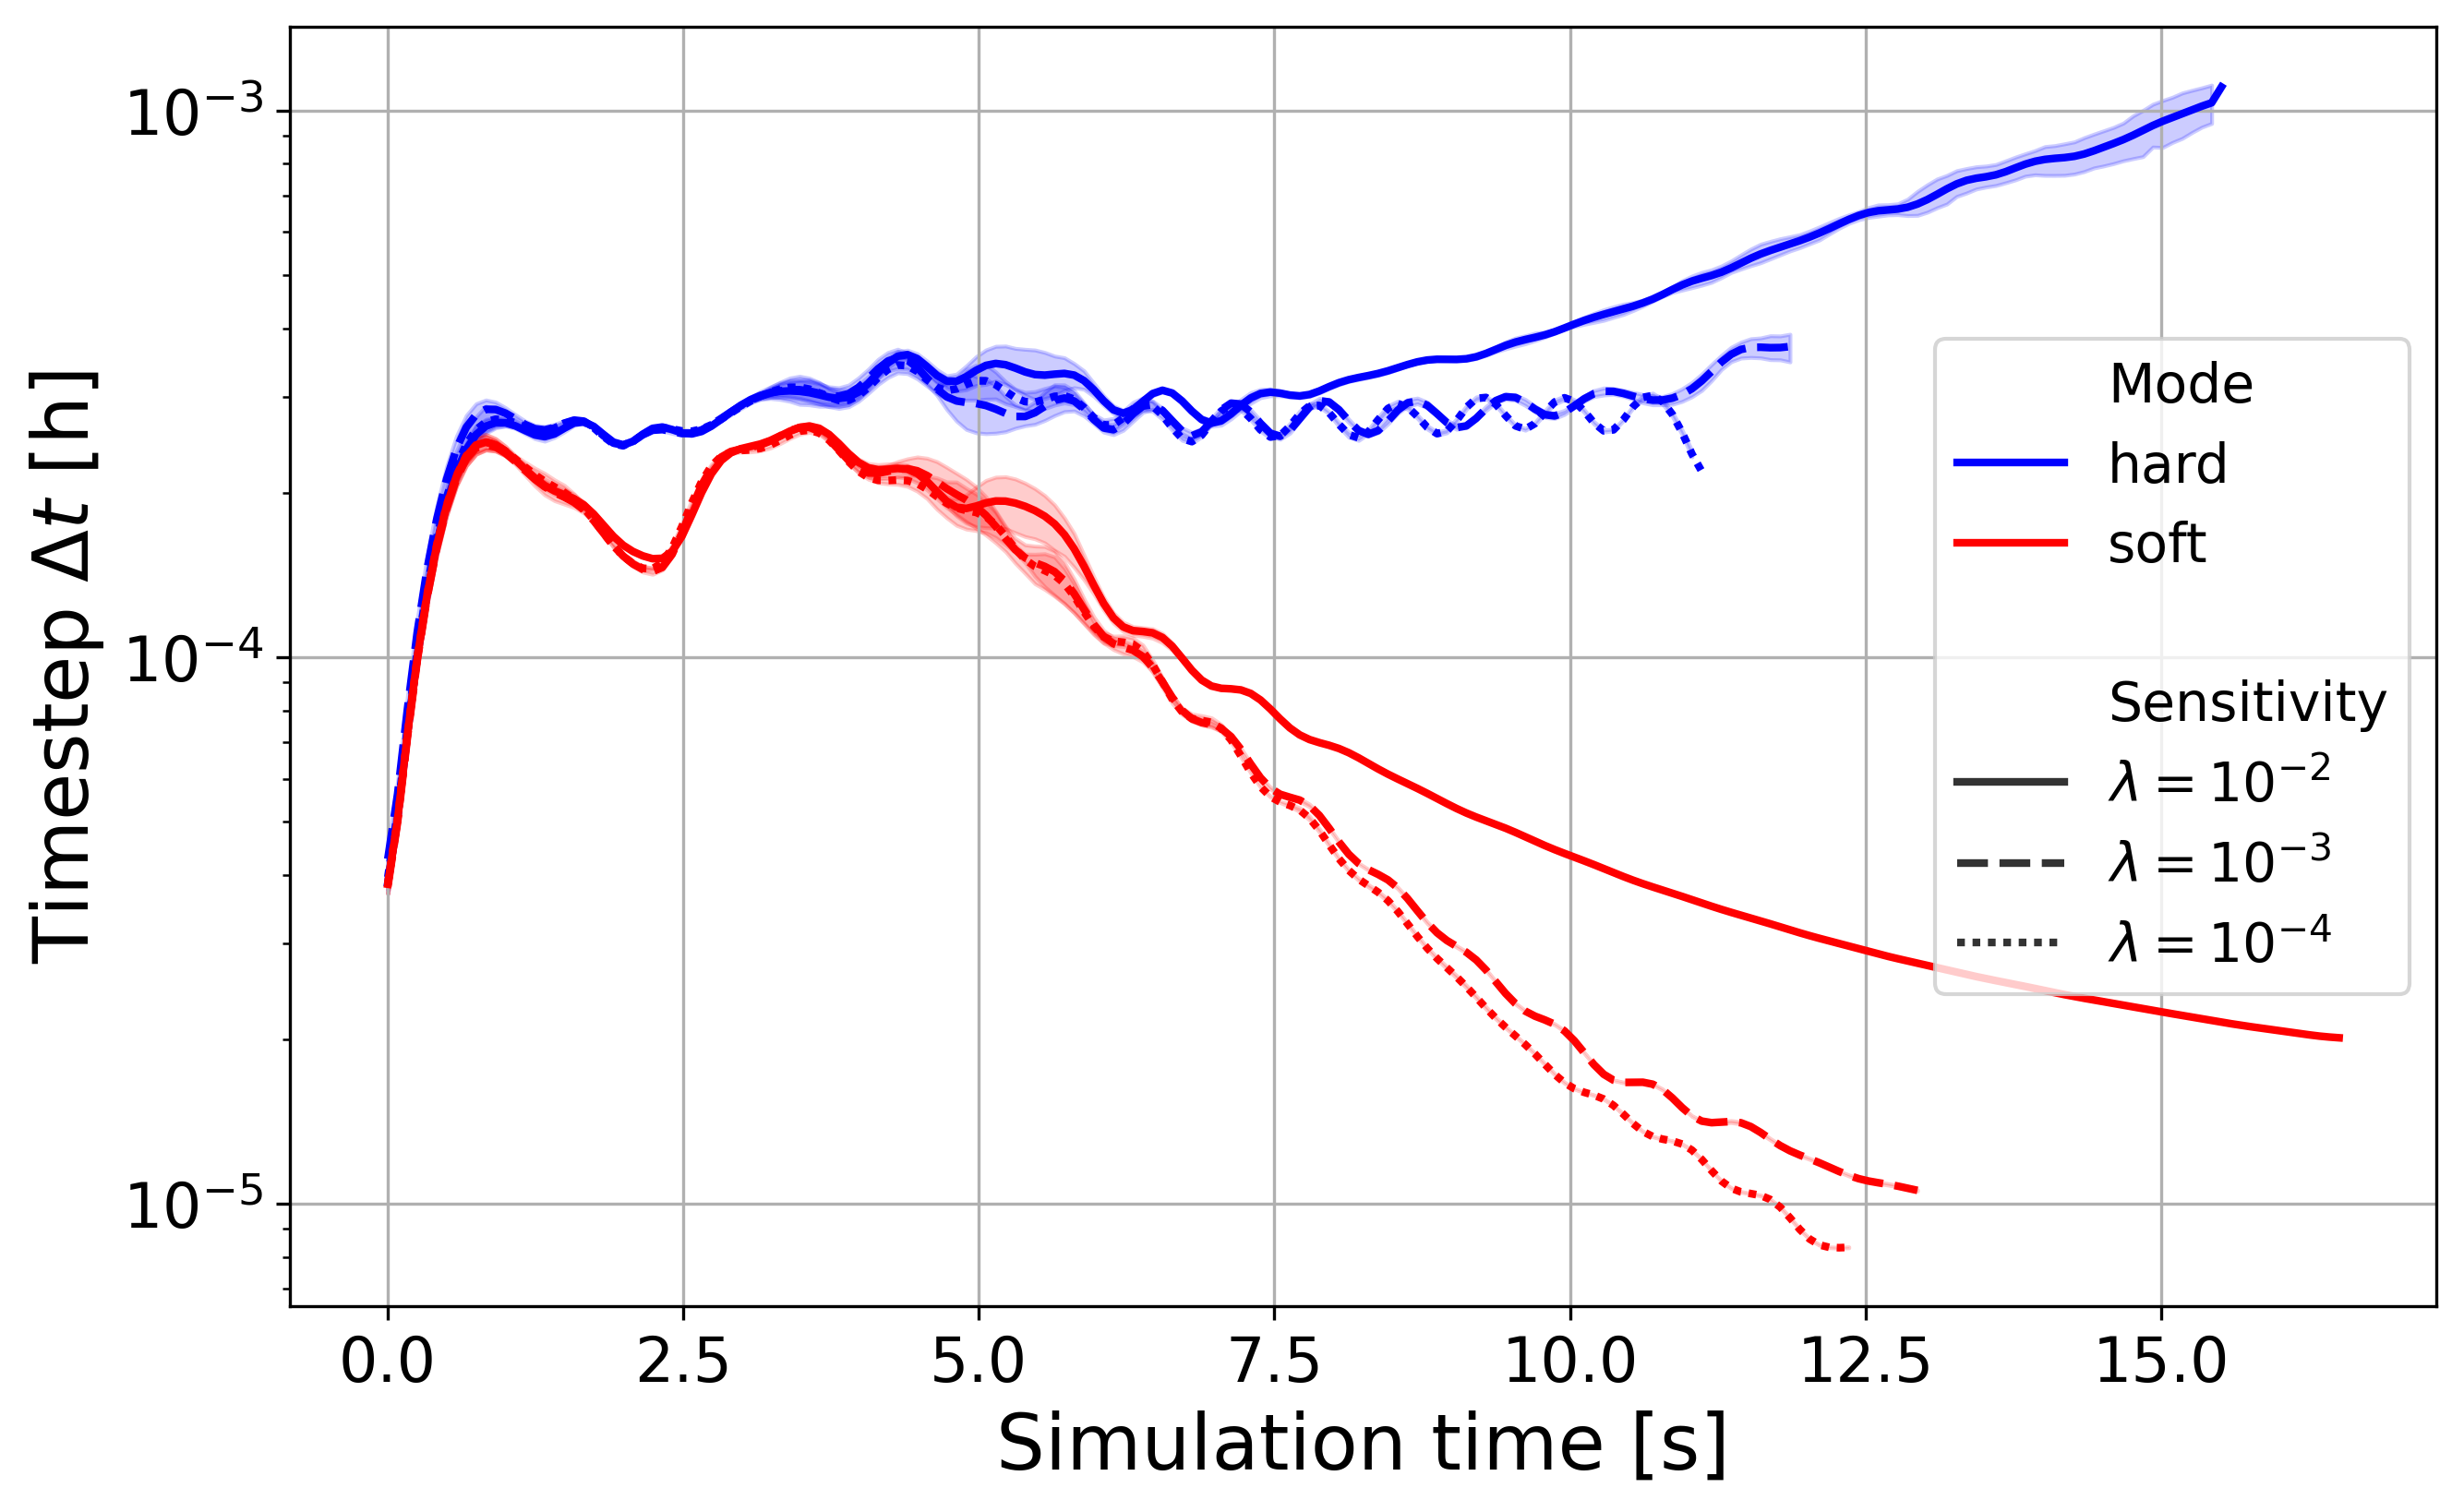
\includegraphics[width=\linewidth]{figures/comparison_plots/combined_simulation_time [s]_vs_dt.png}
    \caption{Adaptive timestep $\Delta t$ over simulation time for both collision models. The hard model stabilizes around ${\Delta t}_{\text{hard}} \approx 3 \cdot 10^{-4} h$, while the soft model decreases to ${\Delta t}_{\text{soft}} \approx 1 \cdot 10^{-5} h$.} \label{fig:simulation_time_vs_dt}
\end{figure}


\subsection{Strong Scaling}
\label{sec:strong_scaling}

To assess the parallel performance of the hard and soft simulation models, we analyze runtime and speedup as a function of CPU cores. Strong scaling tests start from a single cell and grow the colony to a radius of 100, revealing how efficiently each model utilizes additional cores.

At lower CPU counts ($\text{ranks}< 2^4$), the hard model is slightly faster than the soft model (\autoref{fig:runtime_hard_soft}), likely due to its ability to take larger time steps. As core counts increase, both models converge to similar runtimes. Speedup analysis (\autoref{fig:speedup_hard_soft}) shows the soft model scales smoothly up to 20x for 112 ranks, while the hard model slows in the mid-range, limiting the speedup to 17.5x at 112 ranks.

A contributing factor to the poor performance of the soft model at low core counts is the unnaturally high packing densities it produces, thus requiring more cells to reach the same colony radius (See \autoref{fig:colony_radius_vs_num_cells}). Even, with an extremly small per-particle cost (See \autoref{fig:walltime_per_particle}), these additional costs, combined with a smaller stable time step (See \autoref{fig:simulation_time_vs_dt}), lead to longer overall runtimes.

Thus, the hard model seems to be a valid alternative especially for smaller core counts, as it can take larger time steps and requires produces no overhead for simulating unphysically dense colonies.


\begin{figure}[H]
    \centering
    \begin{subfigure}[b]{1\linewidth}
        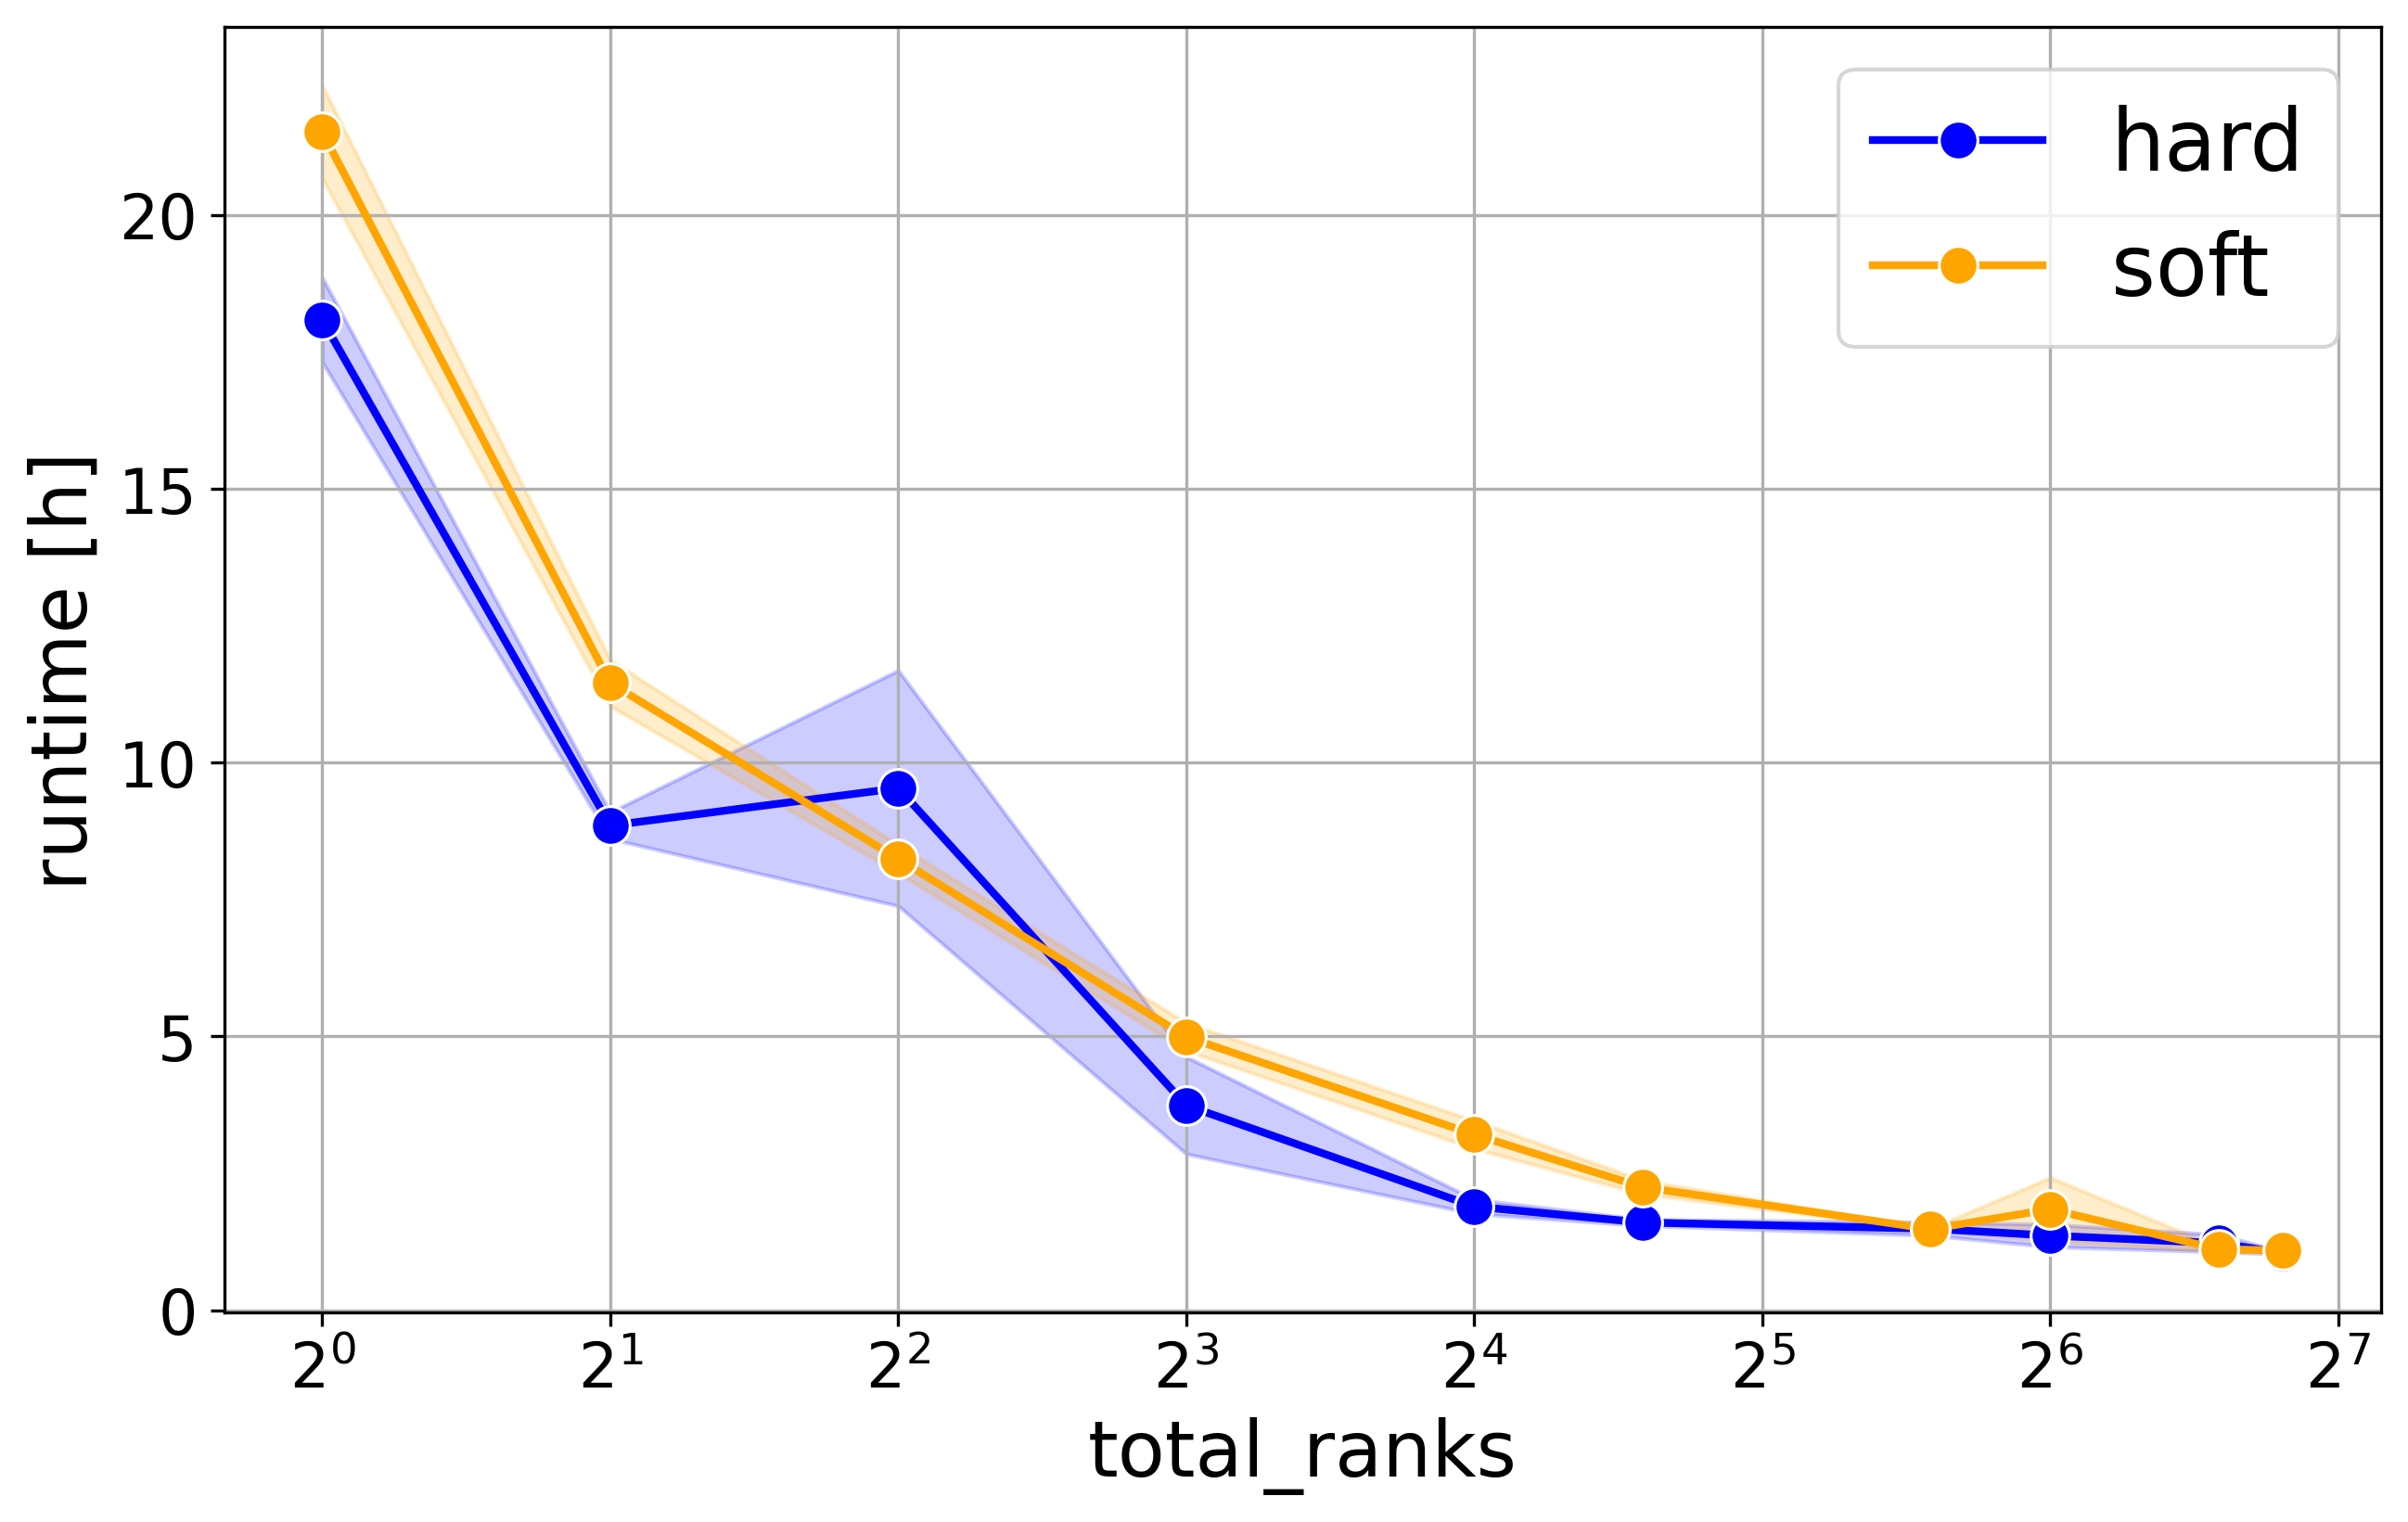
\includegraphics[width=\linewidth]{figures/runtimes/strong_scaling_runtime_hard_soft.png}
        \caption{Runtime vs CPU cores. The hard model is slightly faster at low core counts, but both models converge to similar runtimes at high core counts.}
        \label{fig:runtime_hard_soft}
    \end{subfigure}


    \begin{subfigure}[b]{1\linewidth}
        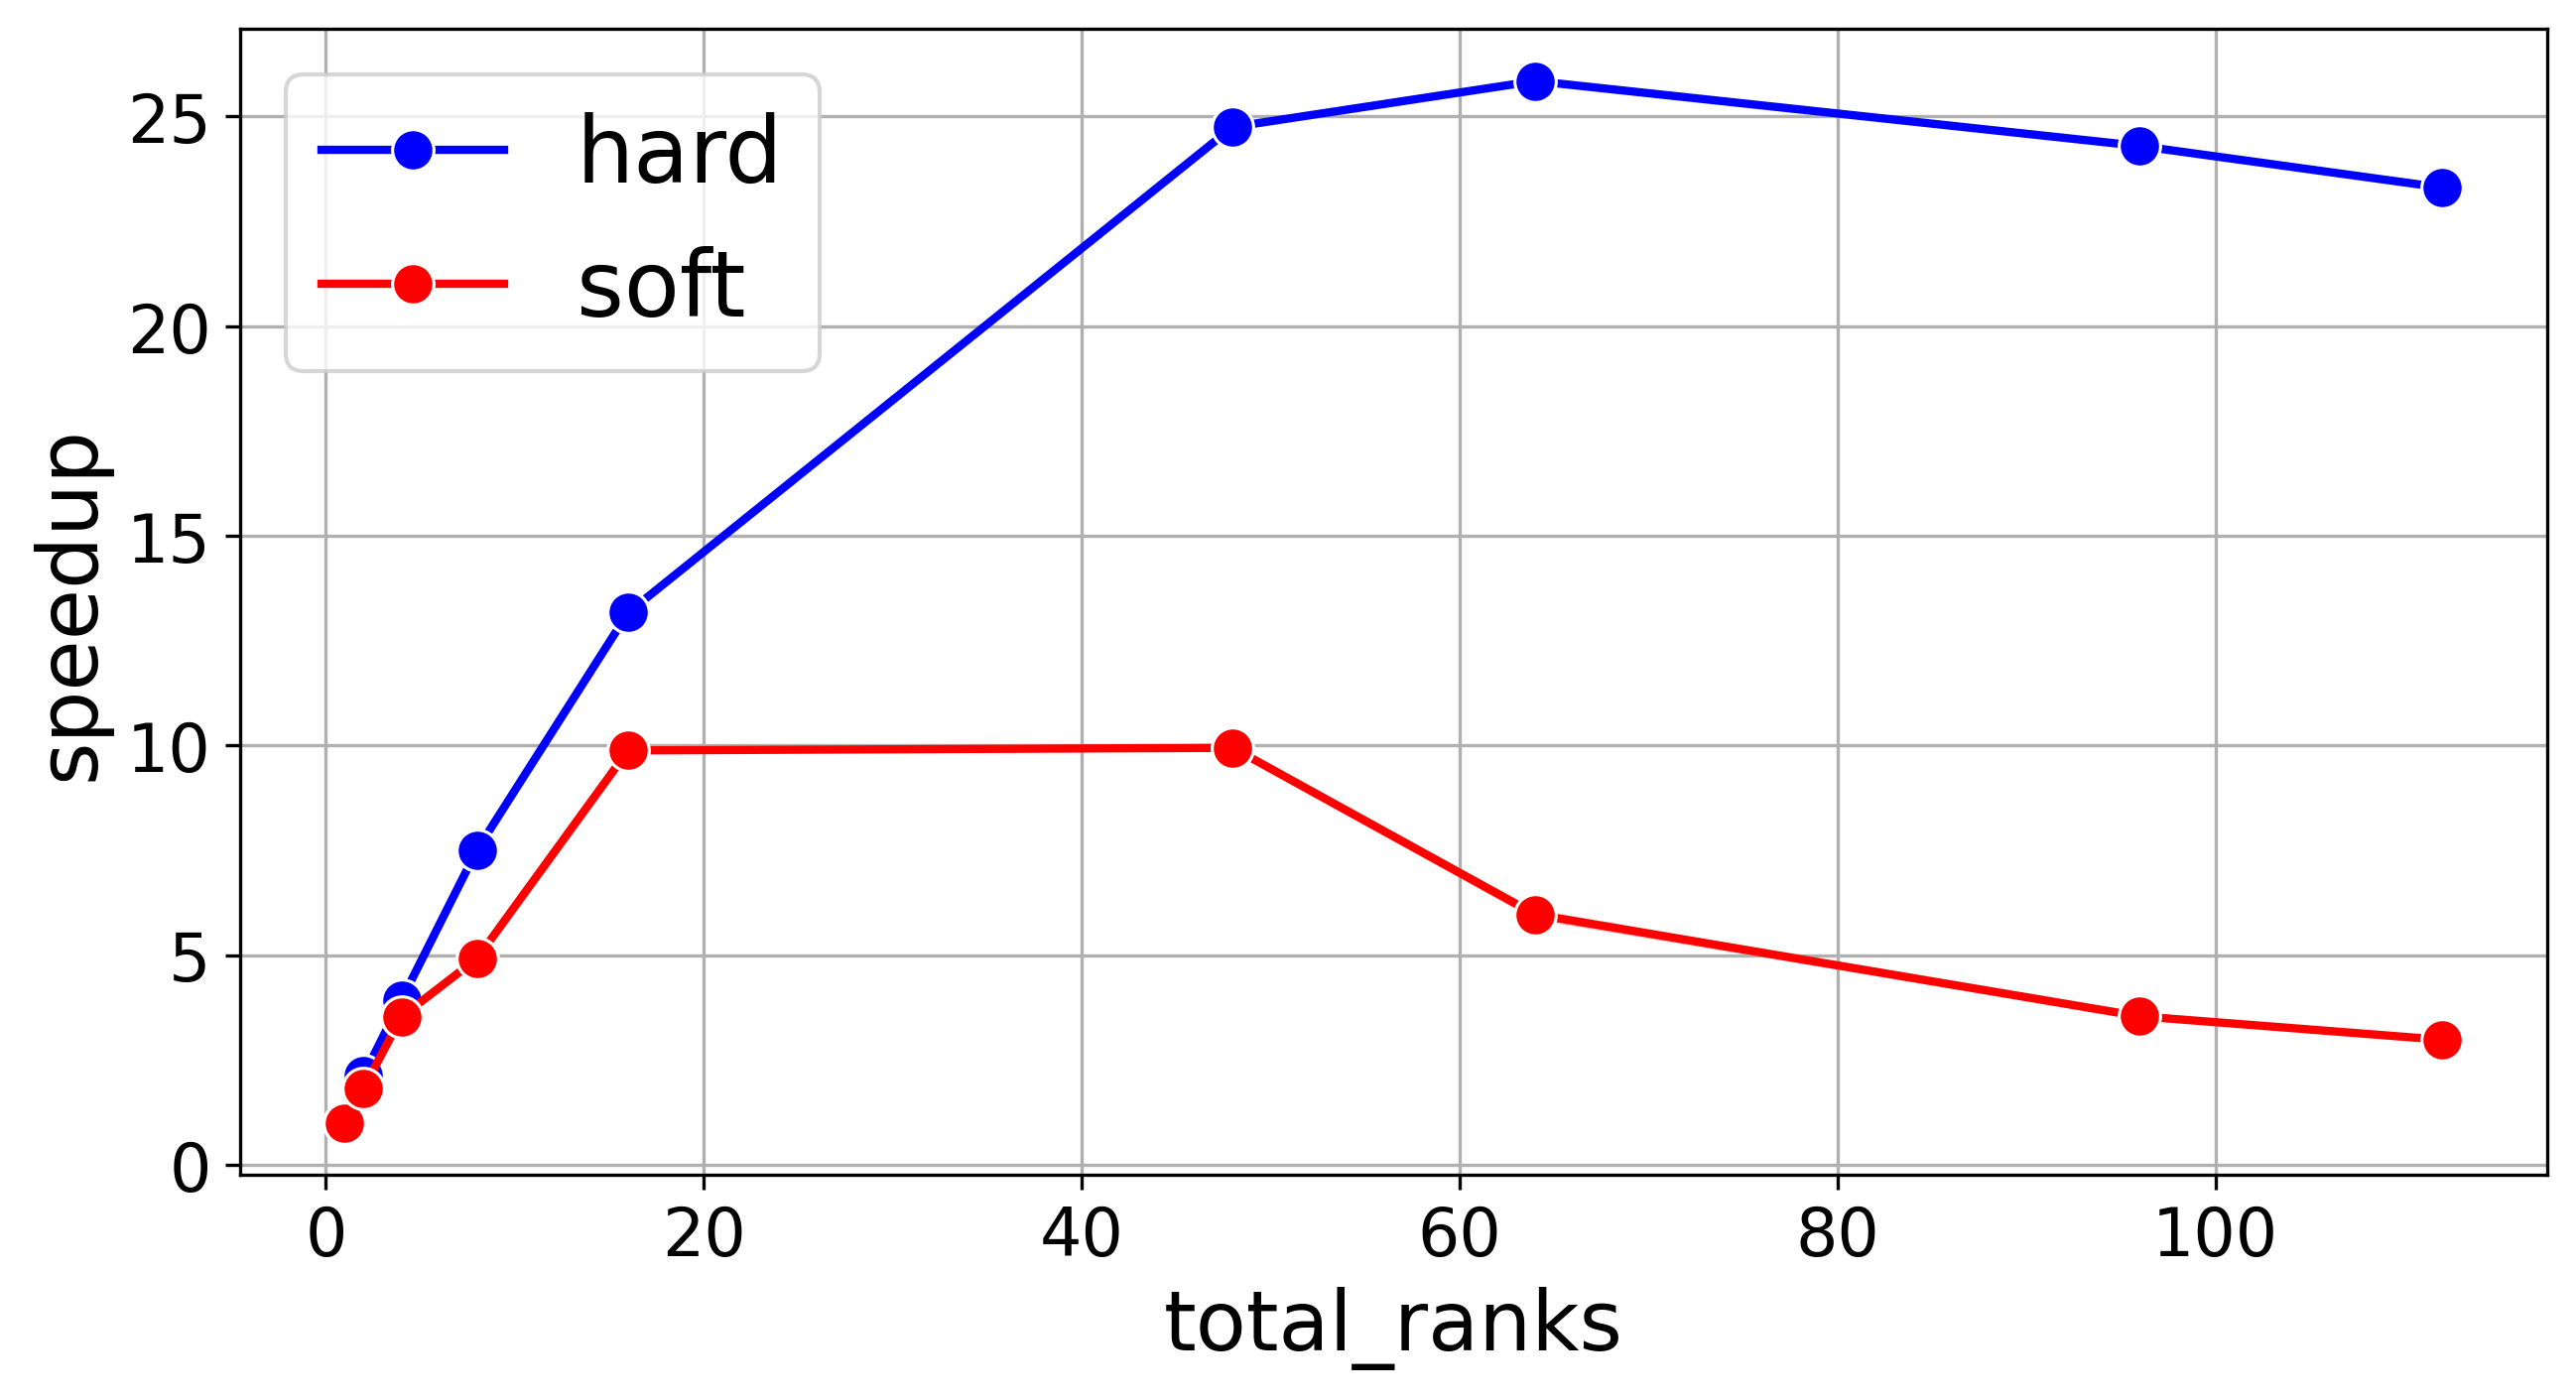
\includegraphics[width=\linewidth]{figures/runtimes/strong_scaling_speedup_hard_soft.png}
        \caption{Speedup vs CPU cores. The soft model scales smoothly up to 20x for 112 ranks, while the hard model slows in the mid-range, limiting speedup to 17.5x at 112 ranks.}
        \label{fig:speedup_hard_soft}
    \end{subfigure}

    \caption{Strong scaling comparison of the hard and soft models.}
\end{figure}

\subsection{Runtime and Scalability Analysis}
\label{sec:complexity_scalability}

This section delves deeper into the computational performance of both collision models by examining the walltime per cell during simulations.

As shown in \autoref{fig:walltime_per_particle}, the per-cell walltime remains approximately constant across each model but is substantially lower for the soft model. This difference arises because the soft model requires only a single force evaluation per cell, whereas the cells in the hard model contribute to global effects. \autoref{fig:walltime_per_particle} also reveals subtle temporal trends: walltime decreases slightly as cell number increases, likely due to improved load balance from domain decomposition, which allows computational cores to process cells more efficiently. Conversely, walltime increases modestly over time, presumably because each cell contributes progressively to global interactions that the solver must resolve.

A possible explanation for the hard model's increased walltime is the higher number of constraints it generates. Each ReLCP iteration introduces new constraints to resolve overlaps, leading to a denser constraint matrix. \autoref{fig:num_constraints} highlights this difference, showing that the soft model generates 6 constraints per cell (one per neighboring pair), while the hard model produces 21 constraints per cell due to the ReLCP procedure.


\begin{figure}[h]
    \centering
    \begin{subfigure}[b]{0.9\linewidth}
        \centering
        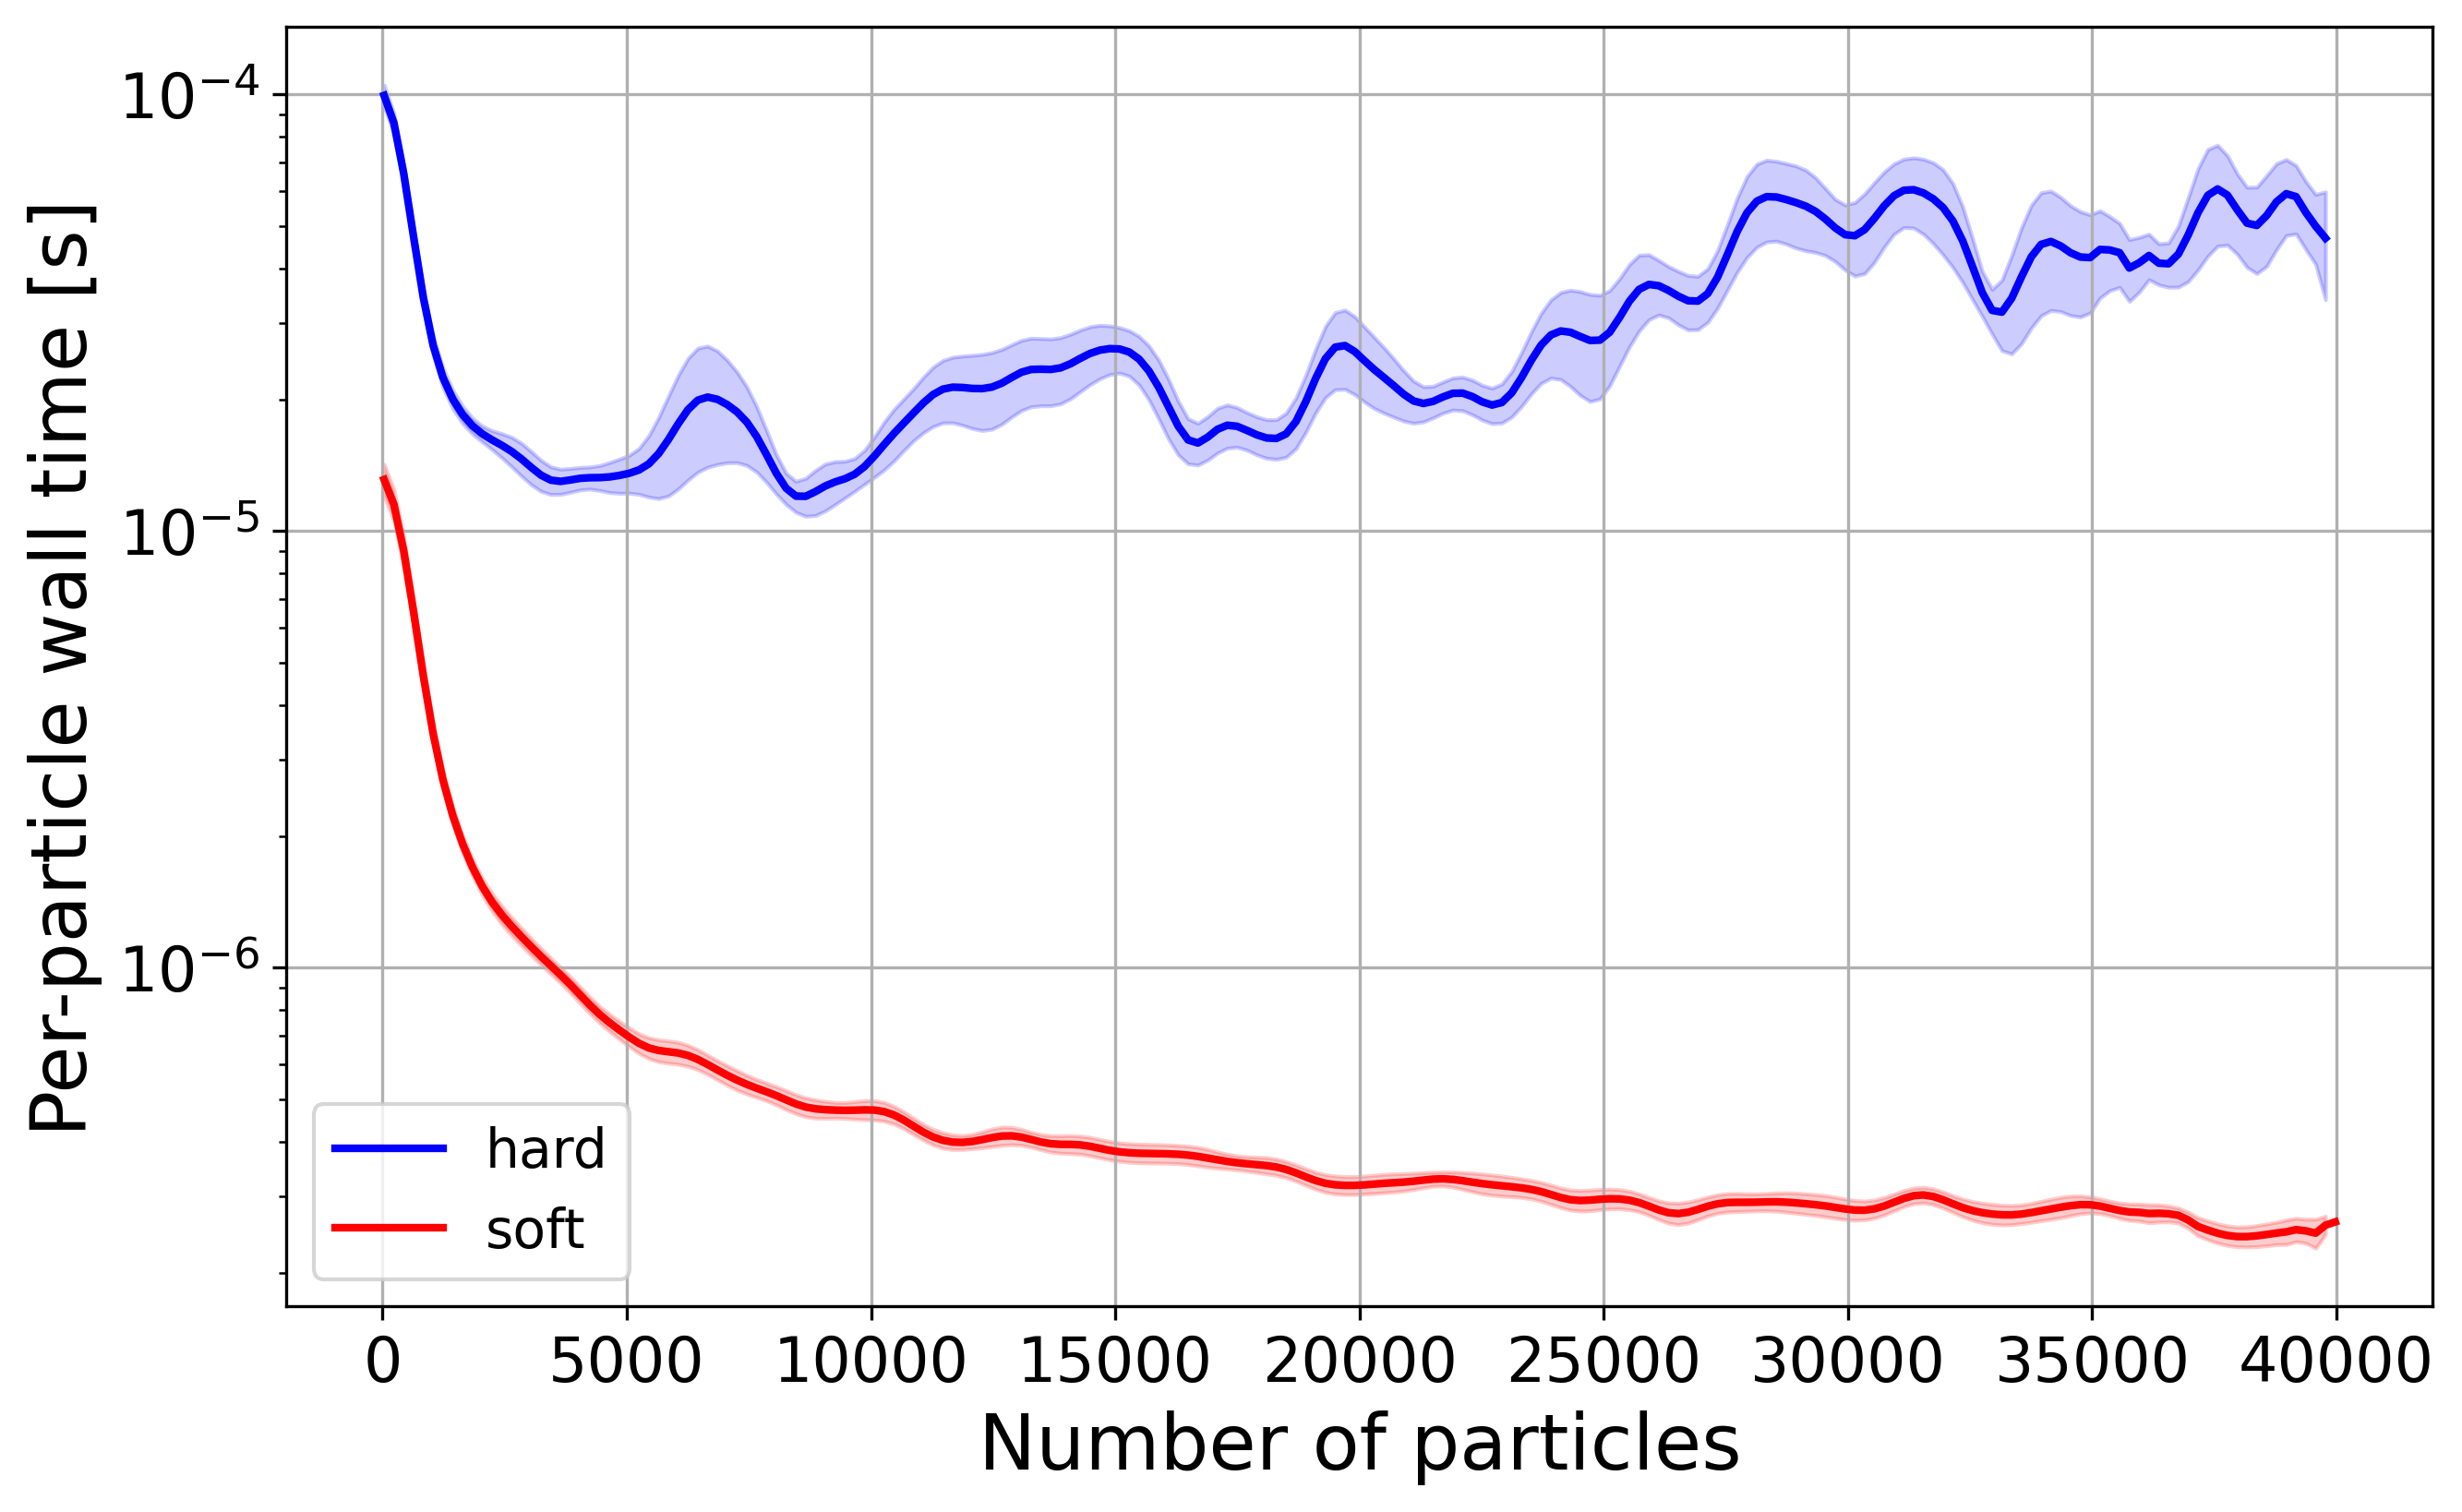
\includegraphics[width=\linewidth]{figures/comparison_plots/combined_num_particles_vs_wall_time_per_particle_with_fit.png}
        \caption{Per-cell walltime for both the hard and soft models with 112 ranks.}
        \label{fig:walltime_per_particle}
    \end{subfigure}


    \begin{subfigure}[b]{0.9\linewidth}
        \centering
        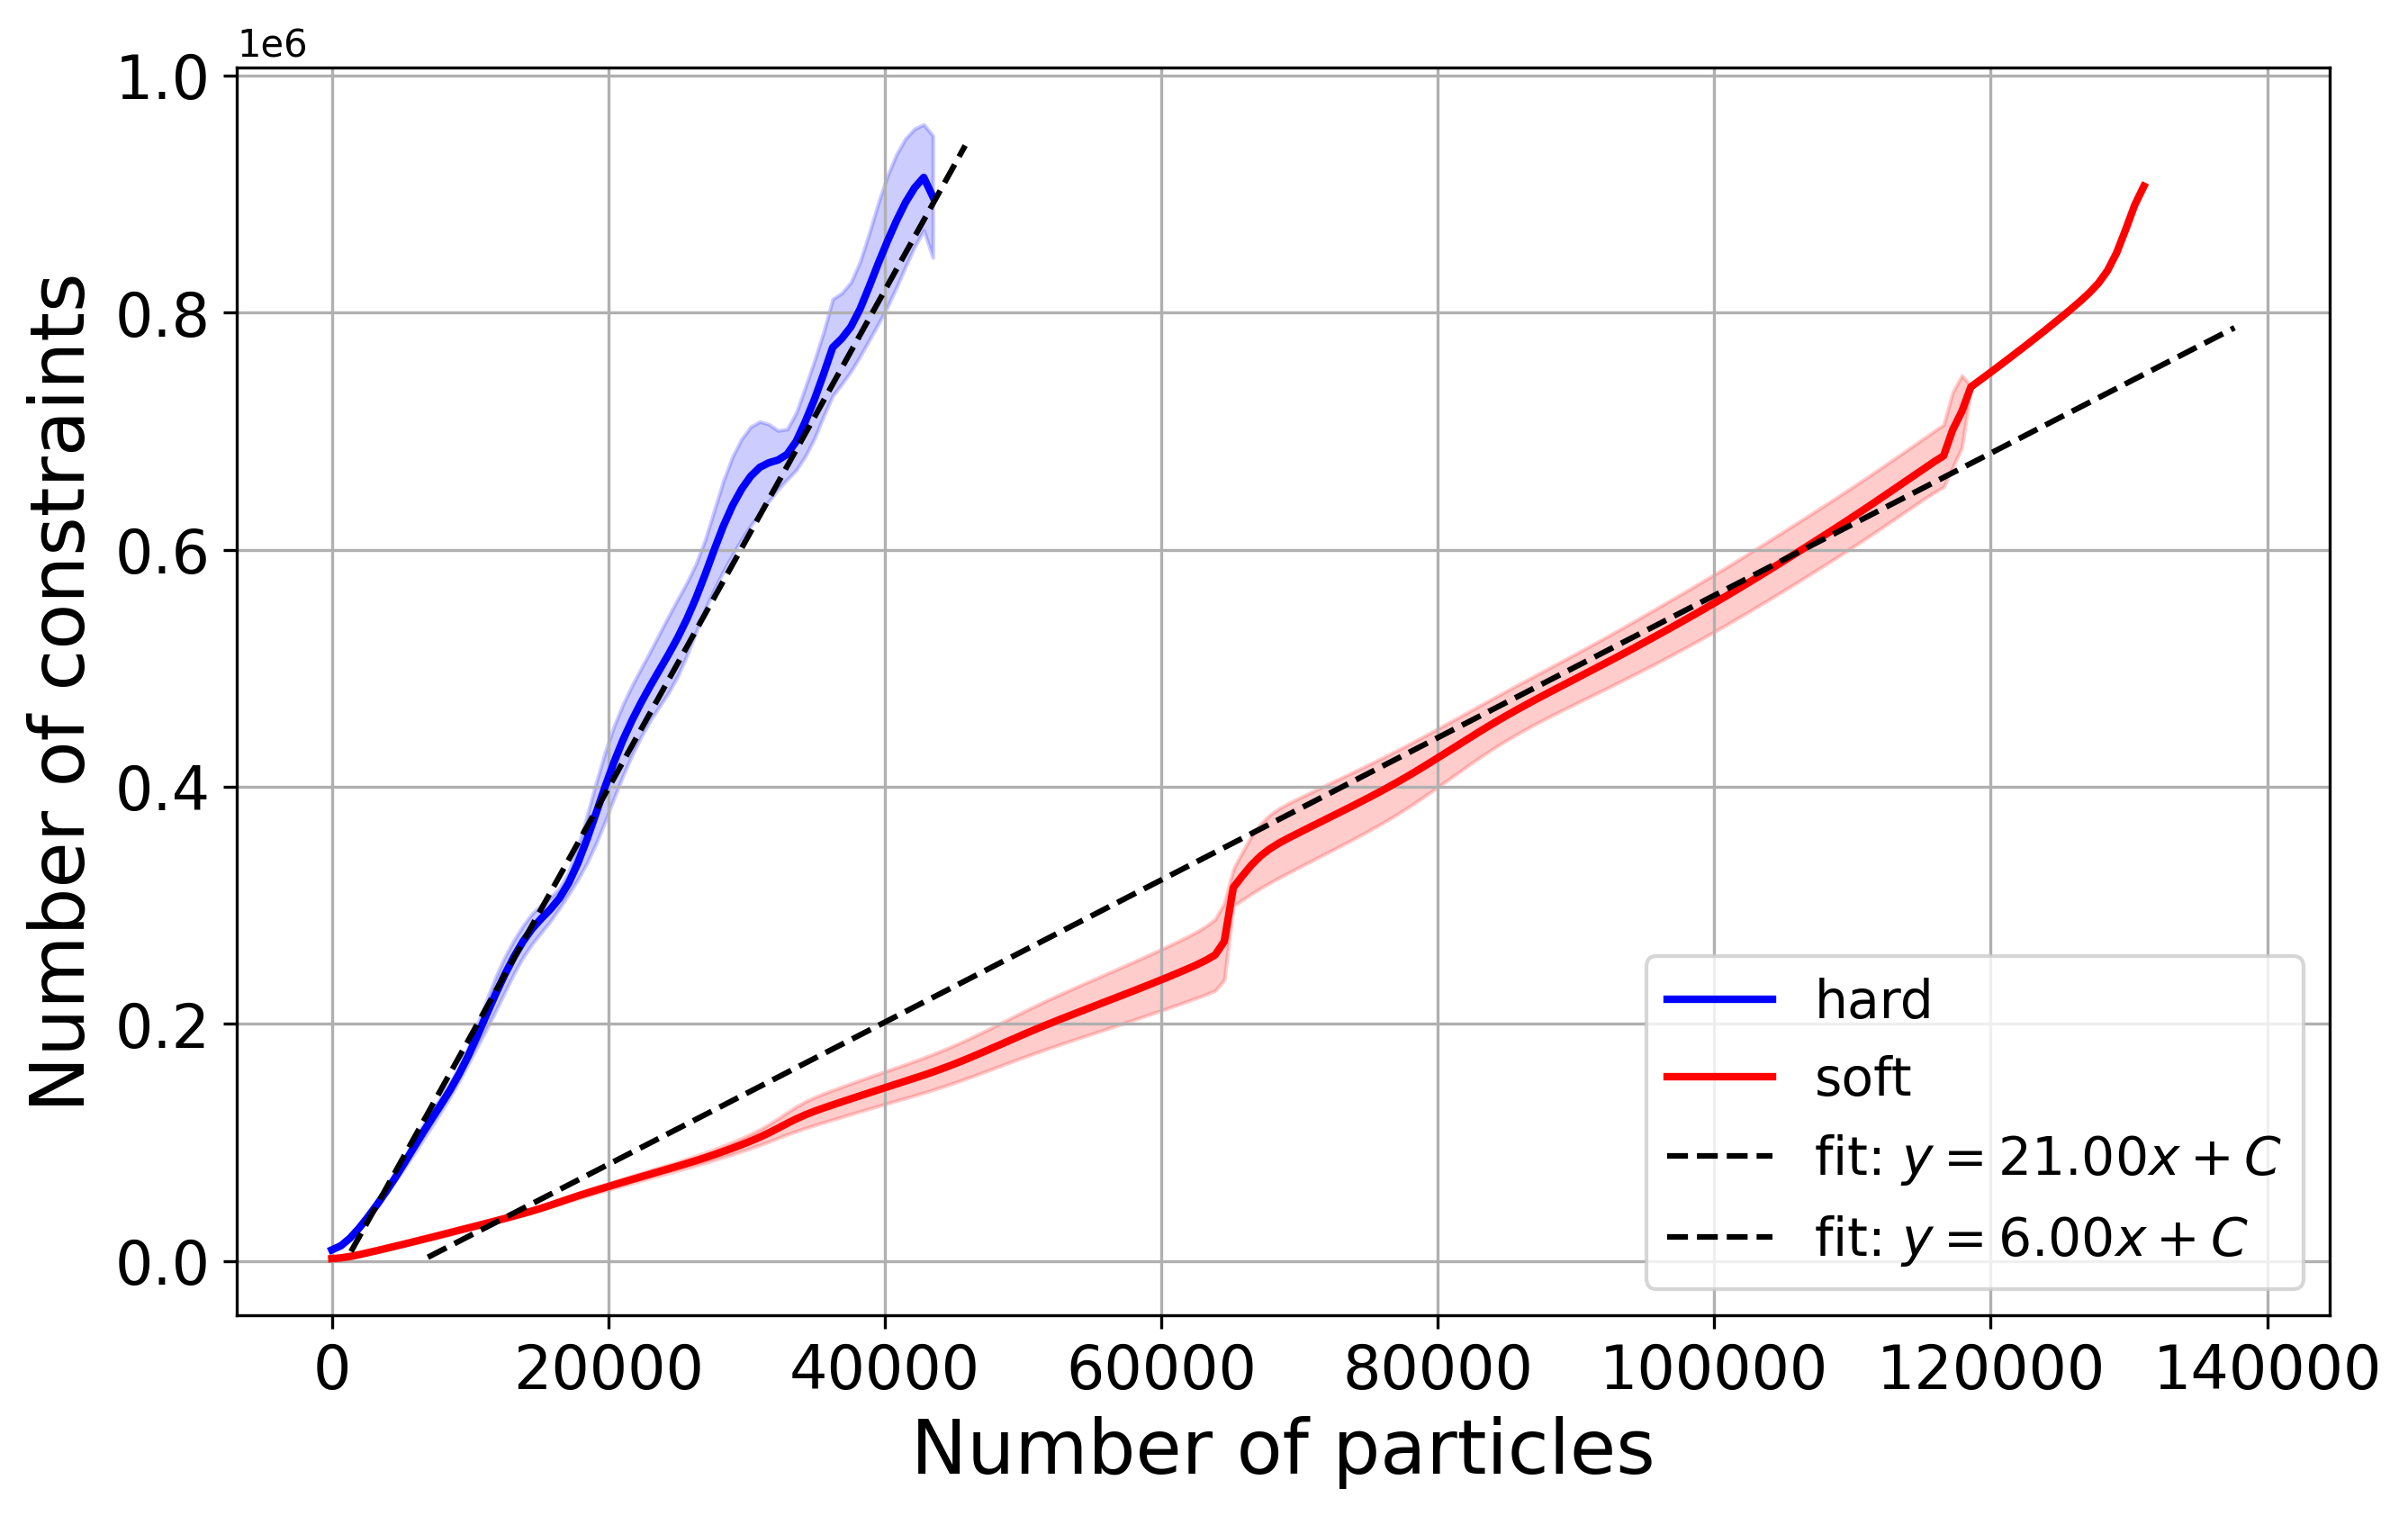
\includegraphics[width=\linewidth]{figures/comparison_plots/combined_num_constraints_vs_num_particles_with_fit.png}
        \caption{Number of constraints as a function of cell count $N$ for both models.}
        \label{fig:num_constraints}
    \end{subfigure}

    \caption{Comparison of simulation metrics for the hard and soft collision models with 112 ranks.}
    \label{fig:comparison_metrics}
\end{figure}


\subsection{Maximum attainable Colony Size}

In this section, we investigate the maximum achievable colony size within a fixed computational budget using the \texttt{CoolMUC-4} high-performance computing cluster\footnote{\texttt{CoolMUC-4} is part of the Linux Cluster at the Leibniz Supercomputing Centre (LRZ). It consists of 106 compute nodes equipped with \textit{Intel Xeon Platinum 8480+ (Sapphire Rapids)} CPUs, each providing 112 cores. For further details, see \url{https://doku.lrz.de/coolmuc-4-1082337877.html}.}. Specifically, we compare the largest attainable colony radius obtained with both the hard and soft models with $\lambda=10^{-3}$ when running on 112 ranks over a wall time of 24 hours. This benchmark was just executed once per model due to the high computational cost, so the results should be interpreted with some caution.


As illustrated in \autoref{fig:huge_wall_time_vs_radius}, the soft interaction model exhibits slightly superior scalability, reaching a maximum colony radius of approximately $R = 210$, compared to $R = 195$ for the hard model. Despite the soft model requiring significantly more particles (approximately $1{,}033{,}108$), it still achieves a marginally larger colony within the same computational constraints. In contrast, the hard model attains its limit with only $168{,}339$ particles.


In the previous section about strong scaling (\autoref{sec:strong_scaling}), we observed that the hard model was generally faster for reaching a colony radius of $R=100$. However, as the colony size increases, the hard model's performance advantage diminishes due to its higher computational cost and the continously increasing complexity of resolving global constraints. This split in the performance curves is also evident in \autoref{fig:huge_wall_time_vs_radius}, where the colony radii curves start to diverge significantly beyond $R=100$.


Interestingly, the macroscopic structural characteristics of both colonies remain largely comparable. As shown in \autoref{fig:huge_length_shared}, the average radial particle length $\langle \text{length} \rangle$ exhibits nearly identical oscillatory patterns in both models. Unfortunately, due to the high number of particles in the soft model, we were unable to create a visual snapshot of the entire colony. However, based on the radial length profiles, we can infer that both models produce similar concentric ring patterns, despite the significant differences in microscopic density. The snapshot of the hard model is provided in \autoref{fig:huge_snapshot_hard} for reference.

\begin{figure}[h]
    \centering
    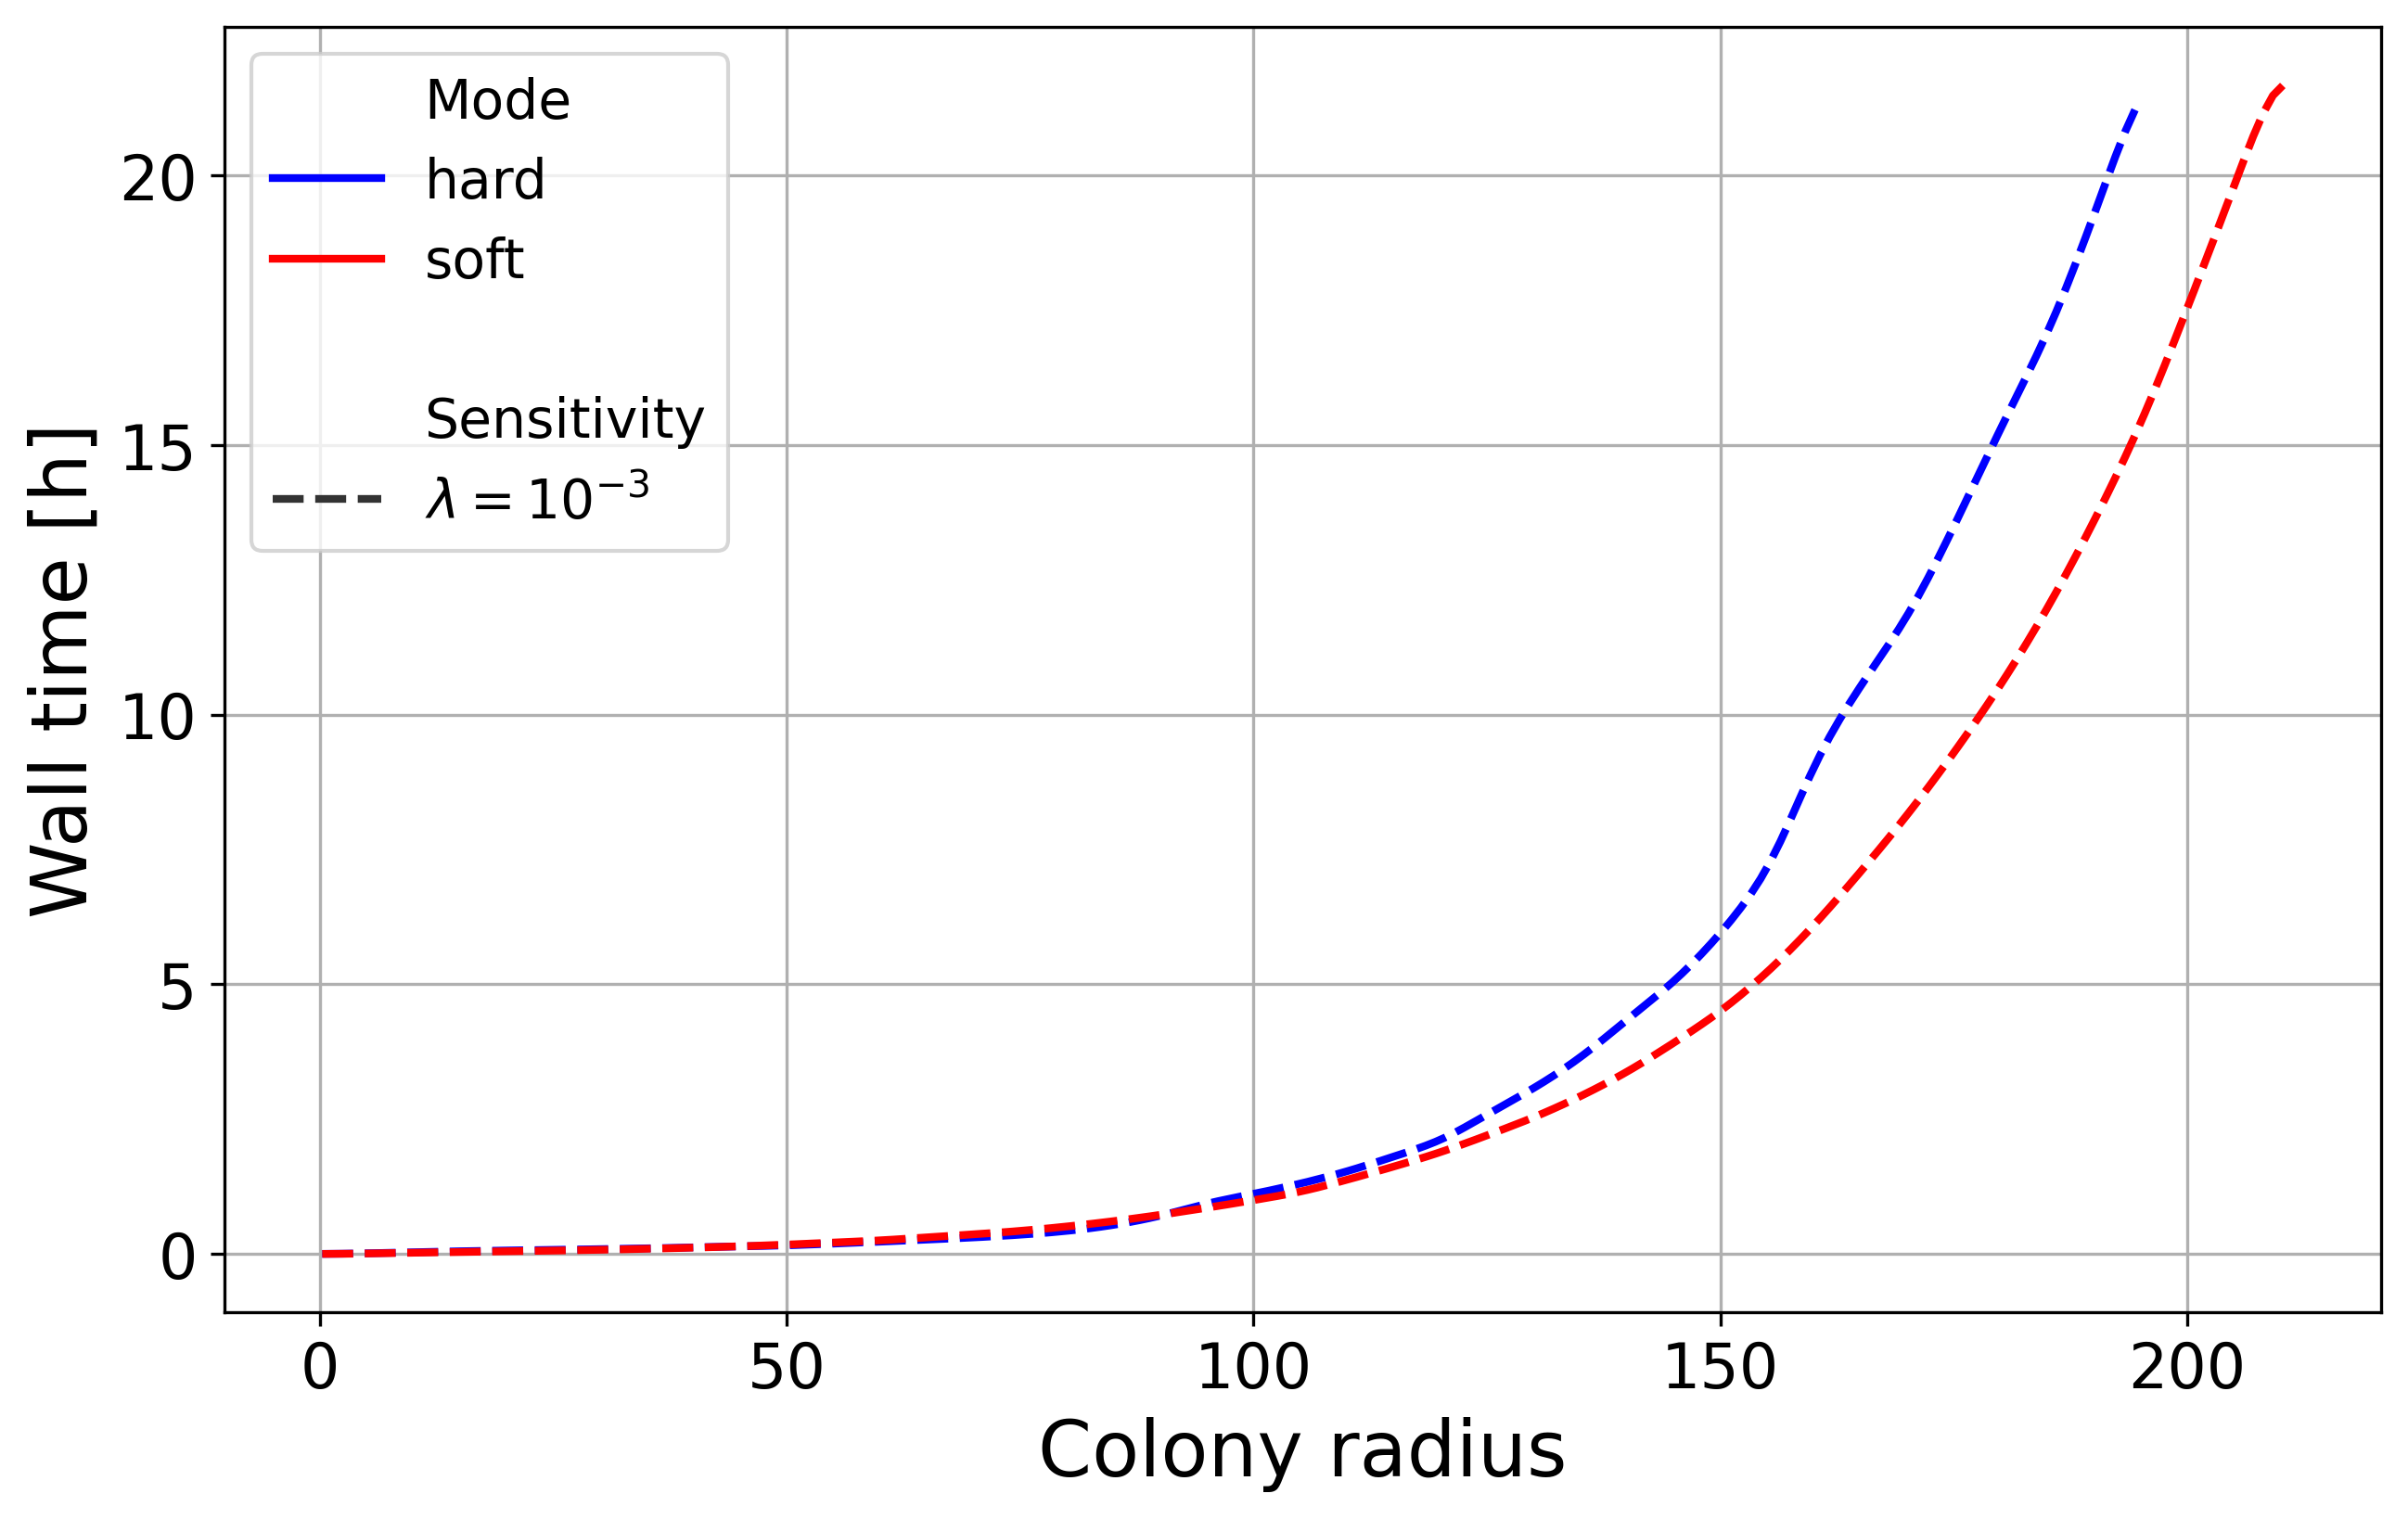
\includegraphics[width=\linewidth]{figures/comparison_plots/huge_wall_time_vs_radius.png}
    \caption{Time evolution of the colony radius for hard and soft interaction modes. Simulations were performed on 112 ranks of the CoolMUC-4 cluster with a maximum wall time of 24 hours. The soft model attains a larger final radius despite higher particle counts. (Sample size: 1 run per model)}
    \label{fig:huge_wall_time_vs_radius}
\end{figure}

\begin{figure}[h]
    \centering
    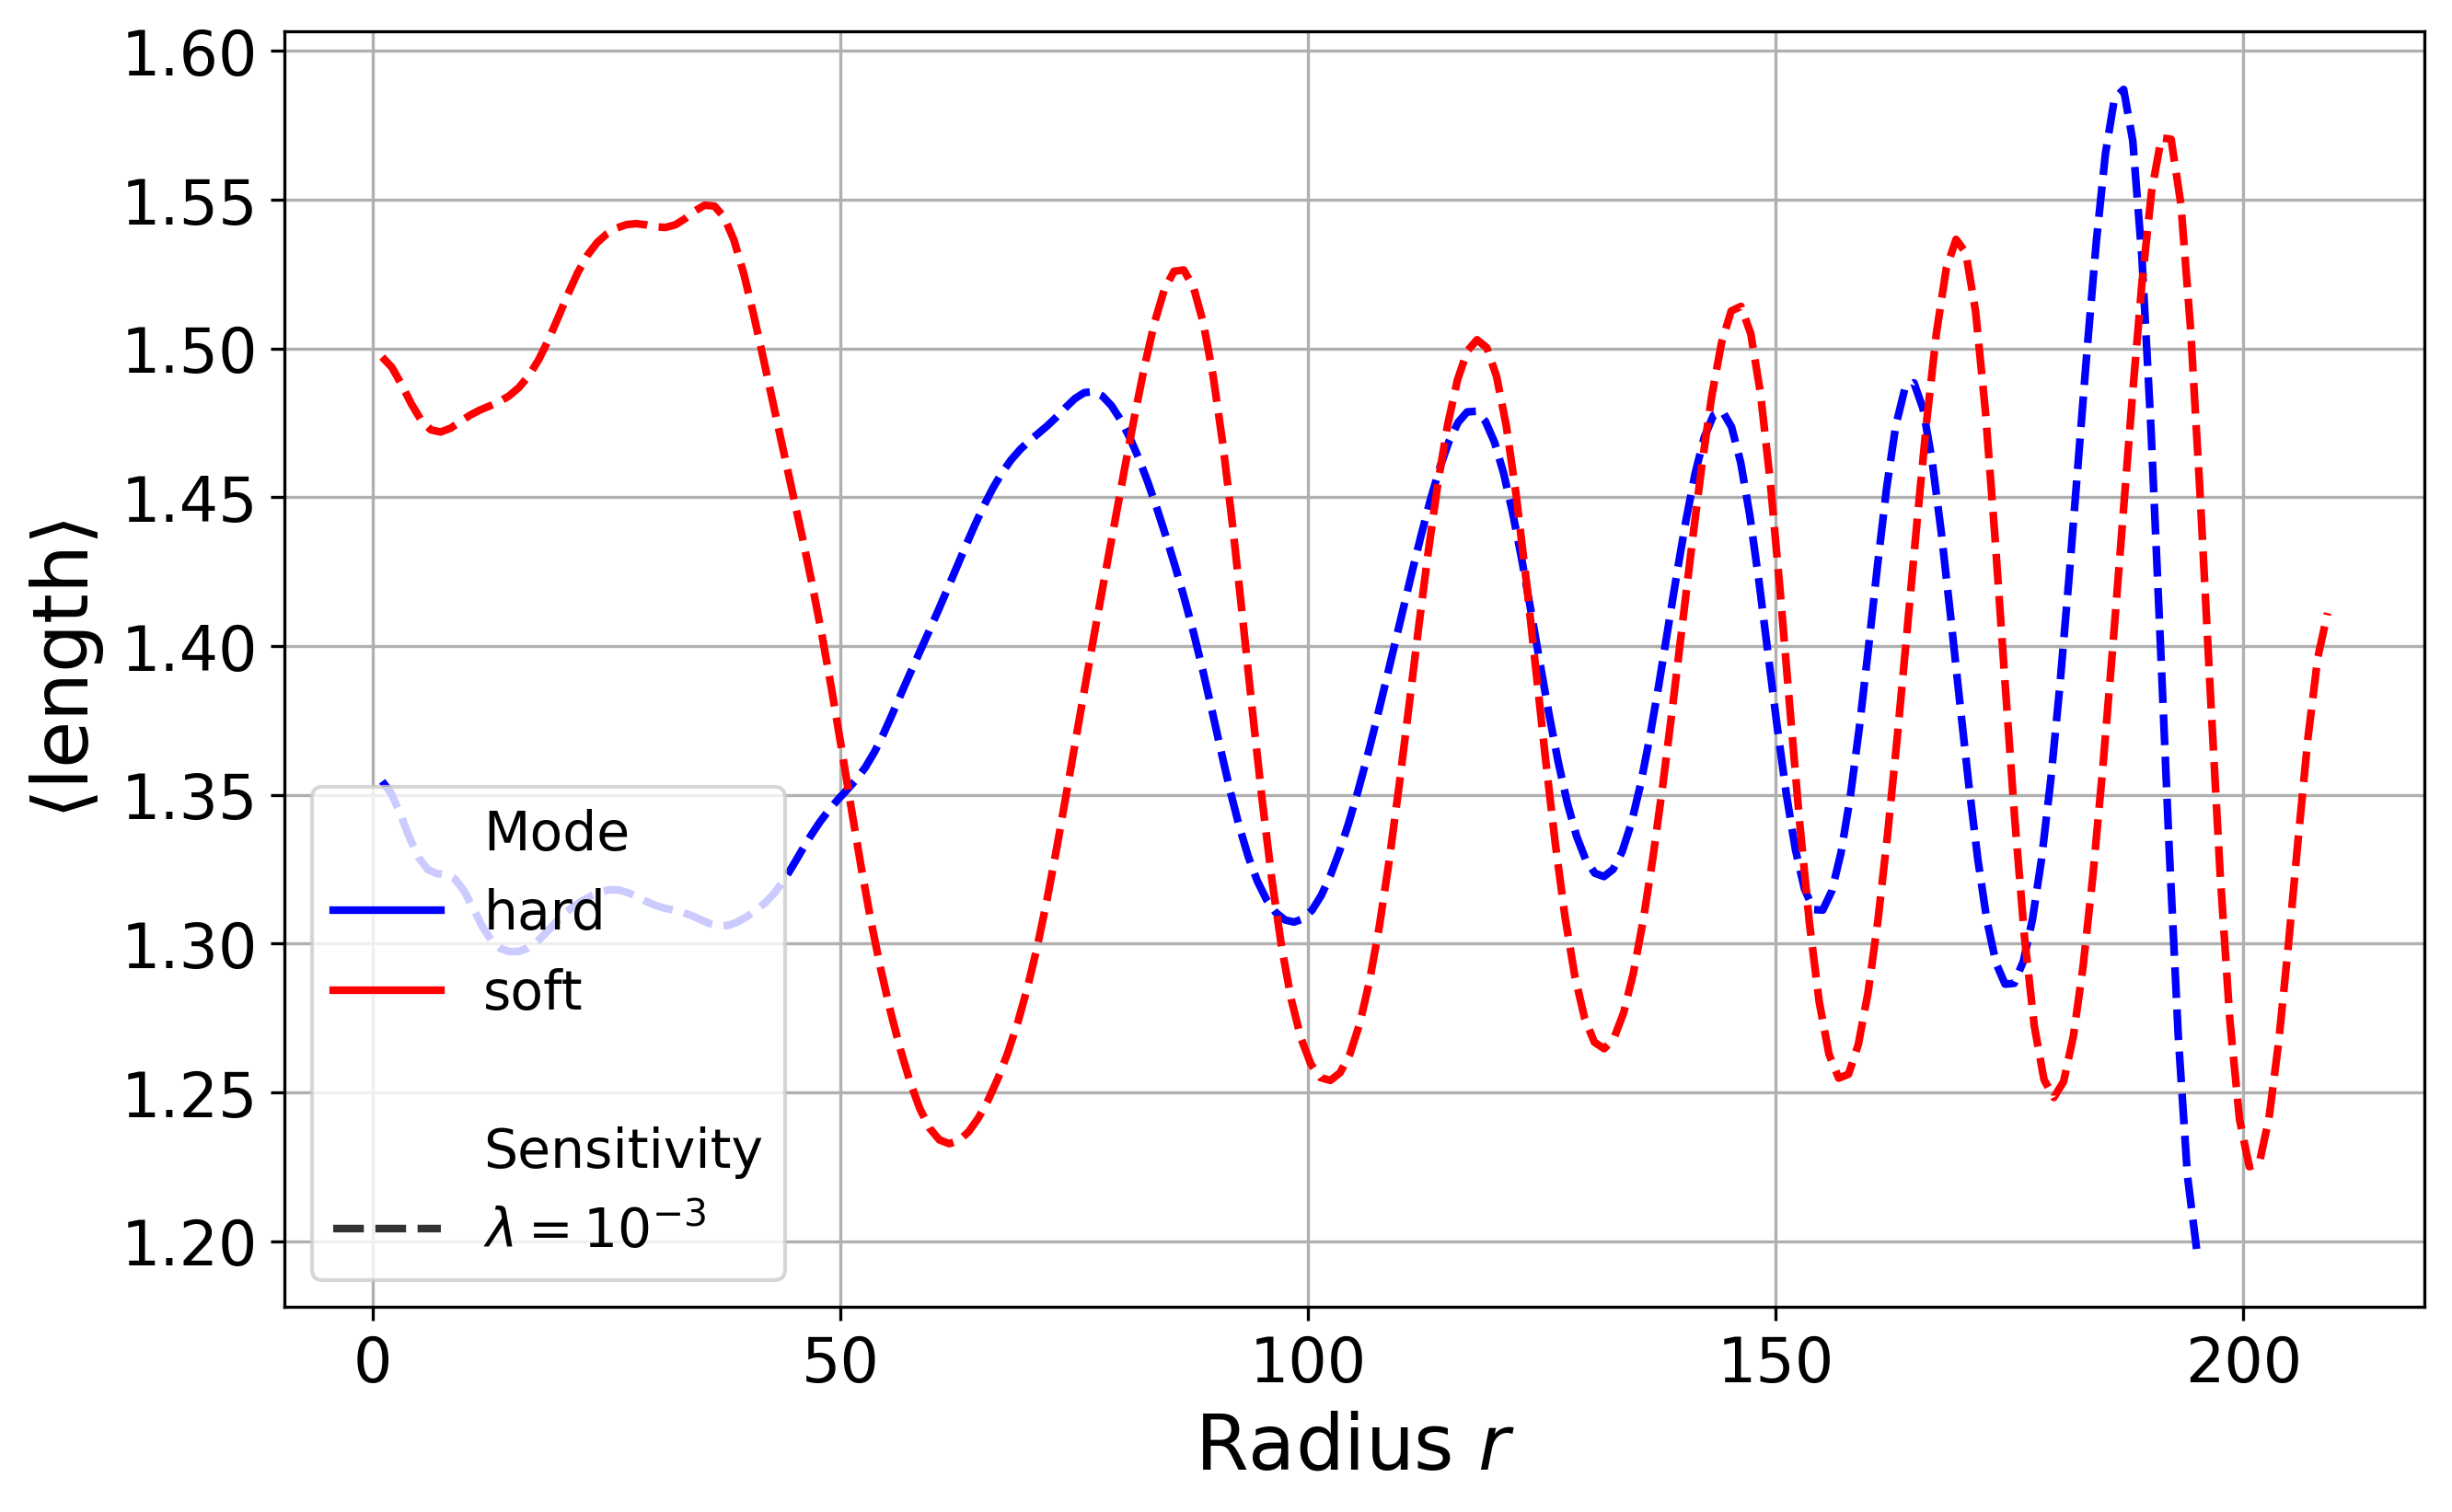
\includegraphics[width=\linewidth]{figures/comparison_plots/huge_length_shared.png}
    \caption{Radial dependence of the average cell length $\langle \text{length} \rangle$ for both models at their maximum attained colony size. Both models exhibit similar oscillatory patterns, indicating comparable macroscopic structure.}
    \label{fig:huge_length_shared}
\end{figure}

Overall, these results demonstrate that the soft interaction model can achieve slightly larger colonies within the same computational budget, despite its higher particle requirements. However, both models produce similar macroscopic patterns, suggesting that either approach can be effectively used for studying large-scale colony growth, depending on whether computational efficiency or adherence to non-overlapping constraints is prioritized.


\subsection{Insights into BBPGD Iterations}


This last section focuses on the performance characteristics of the BBPGD algorithm used in the hard collision model to solve the underlying constrained optimization problem. Understanding the behavior, convergence properties, and computational efficiency of this solver is crucial, as it represents the most computationally intensive component of the overall simulation framework. In the later stages of the simulation, when the system becomes densely packed and a large number of contact constraints must be resolved simultaneously, calls to this function, along with the underlying matrix-vector operations required for gradient evaluations, account for approximately 85\% of the total wall time.

It is therefore essential to analyze how many BBPGD iterations are typically required per time step and how this quantity scales with increasing system size. \autoref{fig:bbpgd_iterations_per_step_vs_num_particles} illustrates that the number of BBPGD iterations remains mostly on the order of $\mathcal{O}(1000)$, with occasional spikes reaching up to $\mathcal{O}(5000)$ during critical moments of the simulation, such as during large-scale rearrangements or near jamming transitions. This number includes additional BBPGD calls arising from the ReLCP procedure, which just requires up to 11 iterations to fully resolve all remaining overlaps as predicted in~\cite{Weady2024SM}. The typical iteration count per time step is thus consistent with the order of magnitude observed in related studies~\cite{Yan2019}, although our model introduces further complexity due to the collision-growth coupling.

The convergence behavior of the BBPGD algorithm within a single time step is further illustrated in \autoref{fig:bbpgd_residual}. In this example, the solver successfully reaches the desired tolerance of $\epsilon = 10^{-3}$ within approximately 2500 iterations, while continuously reducing the system's energy, as defined in \autoref{eq:energy_function}, as shown in \autoref{fig:bbpgd_energy}. The energy decreases monotonically, confirming that the BBPGD method converges as expected under the projected gradient framework. The residual, however, exhibits a highly oscillatory pattern, which is a well-known characteristic of the BBPGD algorithm caused by the adaptive step size selection~\cite{BBPGD,Schneider2021}.

Nevertheless, it remains unclear whether the current interplay between the adaptive time-stepping scheme (\autoref{alg:adaptive_dt}) and the BBPGD solver is fully optimal. Future work could explore more sophisticated adaptive time-stepping strategies that incorporate feedback from the solver, for example by adjusting $\Delta t$ based on the number of BBPGD iterations required in the previous time step. A further line of investigation could assess whether using smaller time steps and thus requiring fewer BBPGD iterations per step might ultimately reduce total runtime, despite the increased number of integration steps. Additionally, exploring warm-start or initialization strategies for the BBPGD solver, possibly by leveraging information from the solution at the previous time step, could significantly accelerate convergence.

\begin{figure}[h]
    \centering
    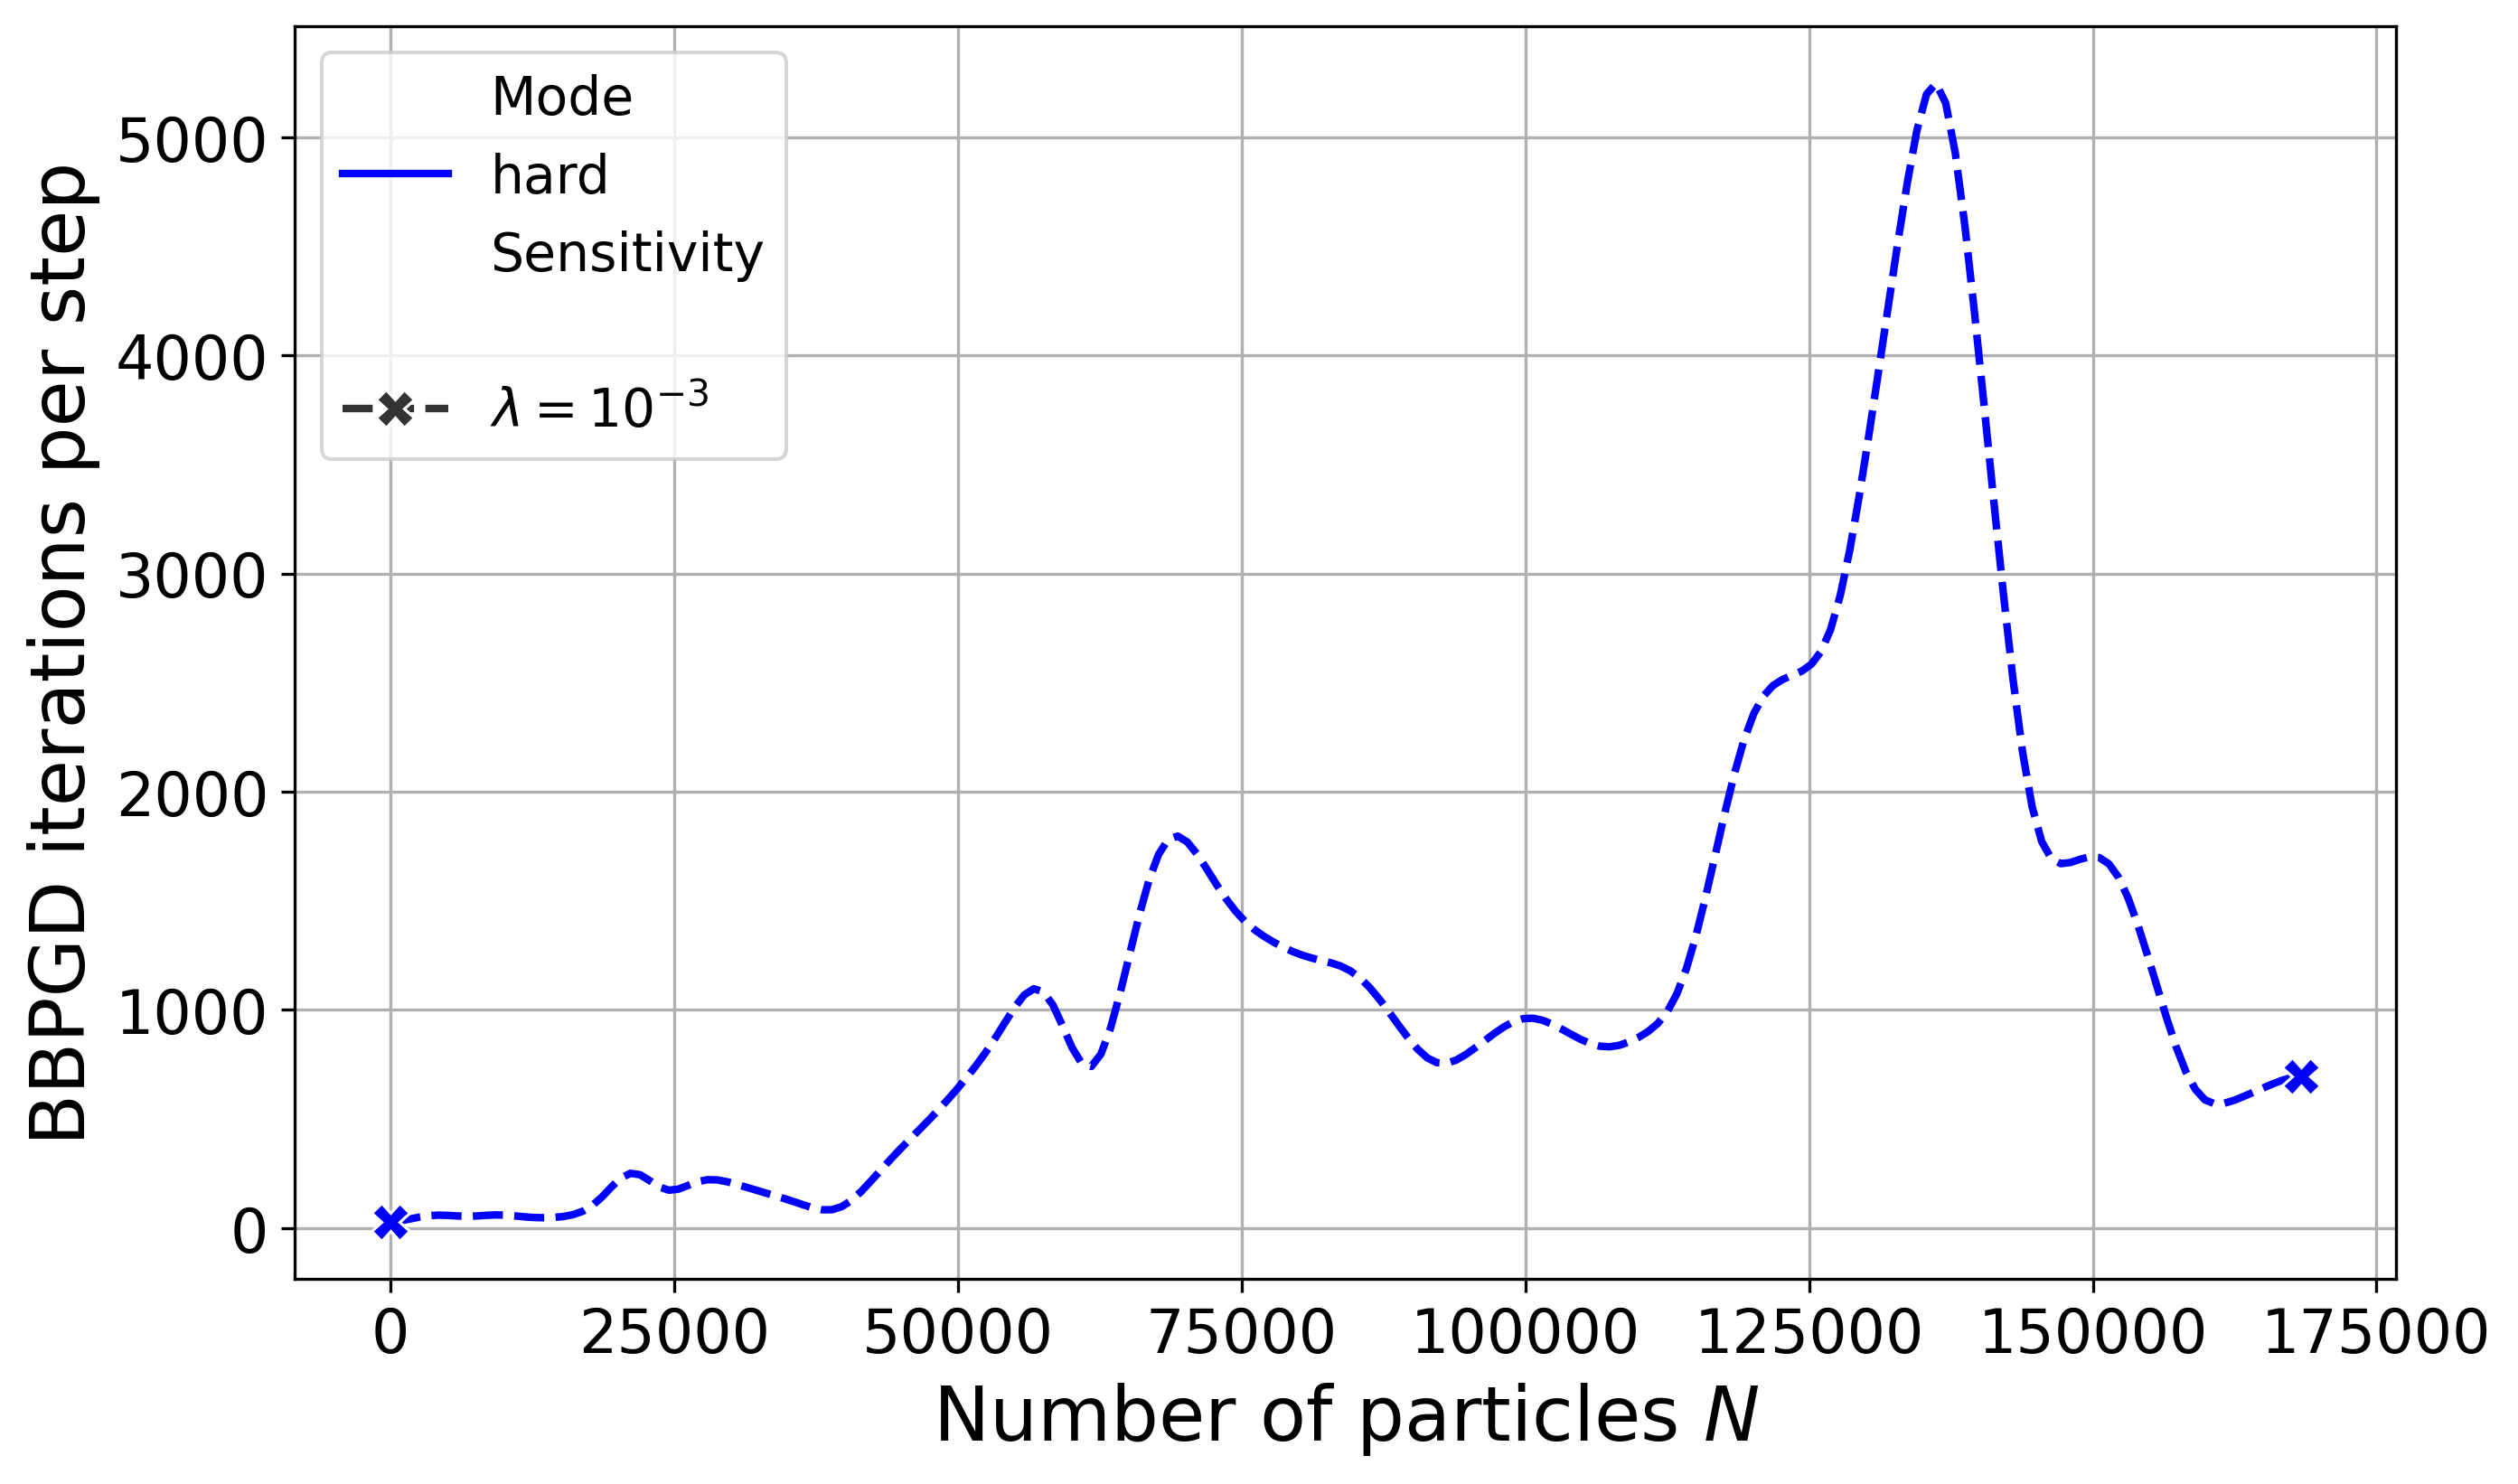
\includegraphics[width=\linewidth]{figures/comparison_plots/bbpgd_num_particles_vs_bbpgd_steps.png}
    \caption{Number of BBPGD iterations per time step as a function of the number of particles in the system. The number of iterations remains roughly around $\mathcal{O}(1000)$, with occasional spikes up to $\mathcal{O}(5000)$ at critical points in the simulation.}
    \label{fig:bbpgd_iterations_per_step_vs_num_particles}
\end{figure}

\begin{figure}[H]
    \centering
    \begin{subfigure}[b]{\linewidth}
        \centering
        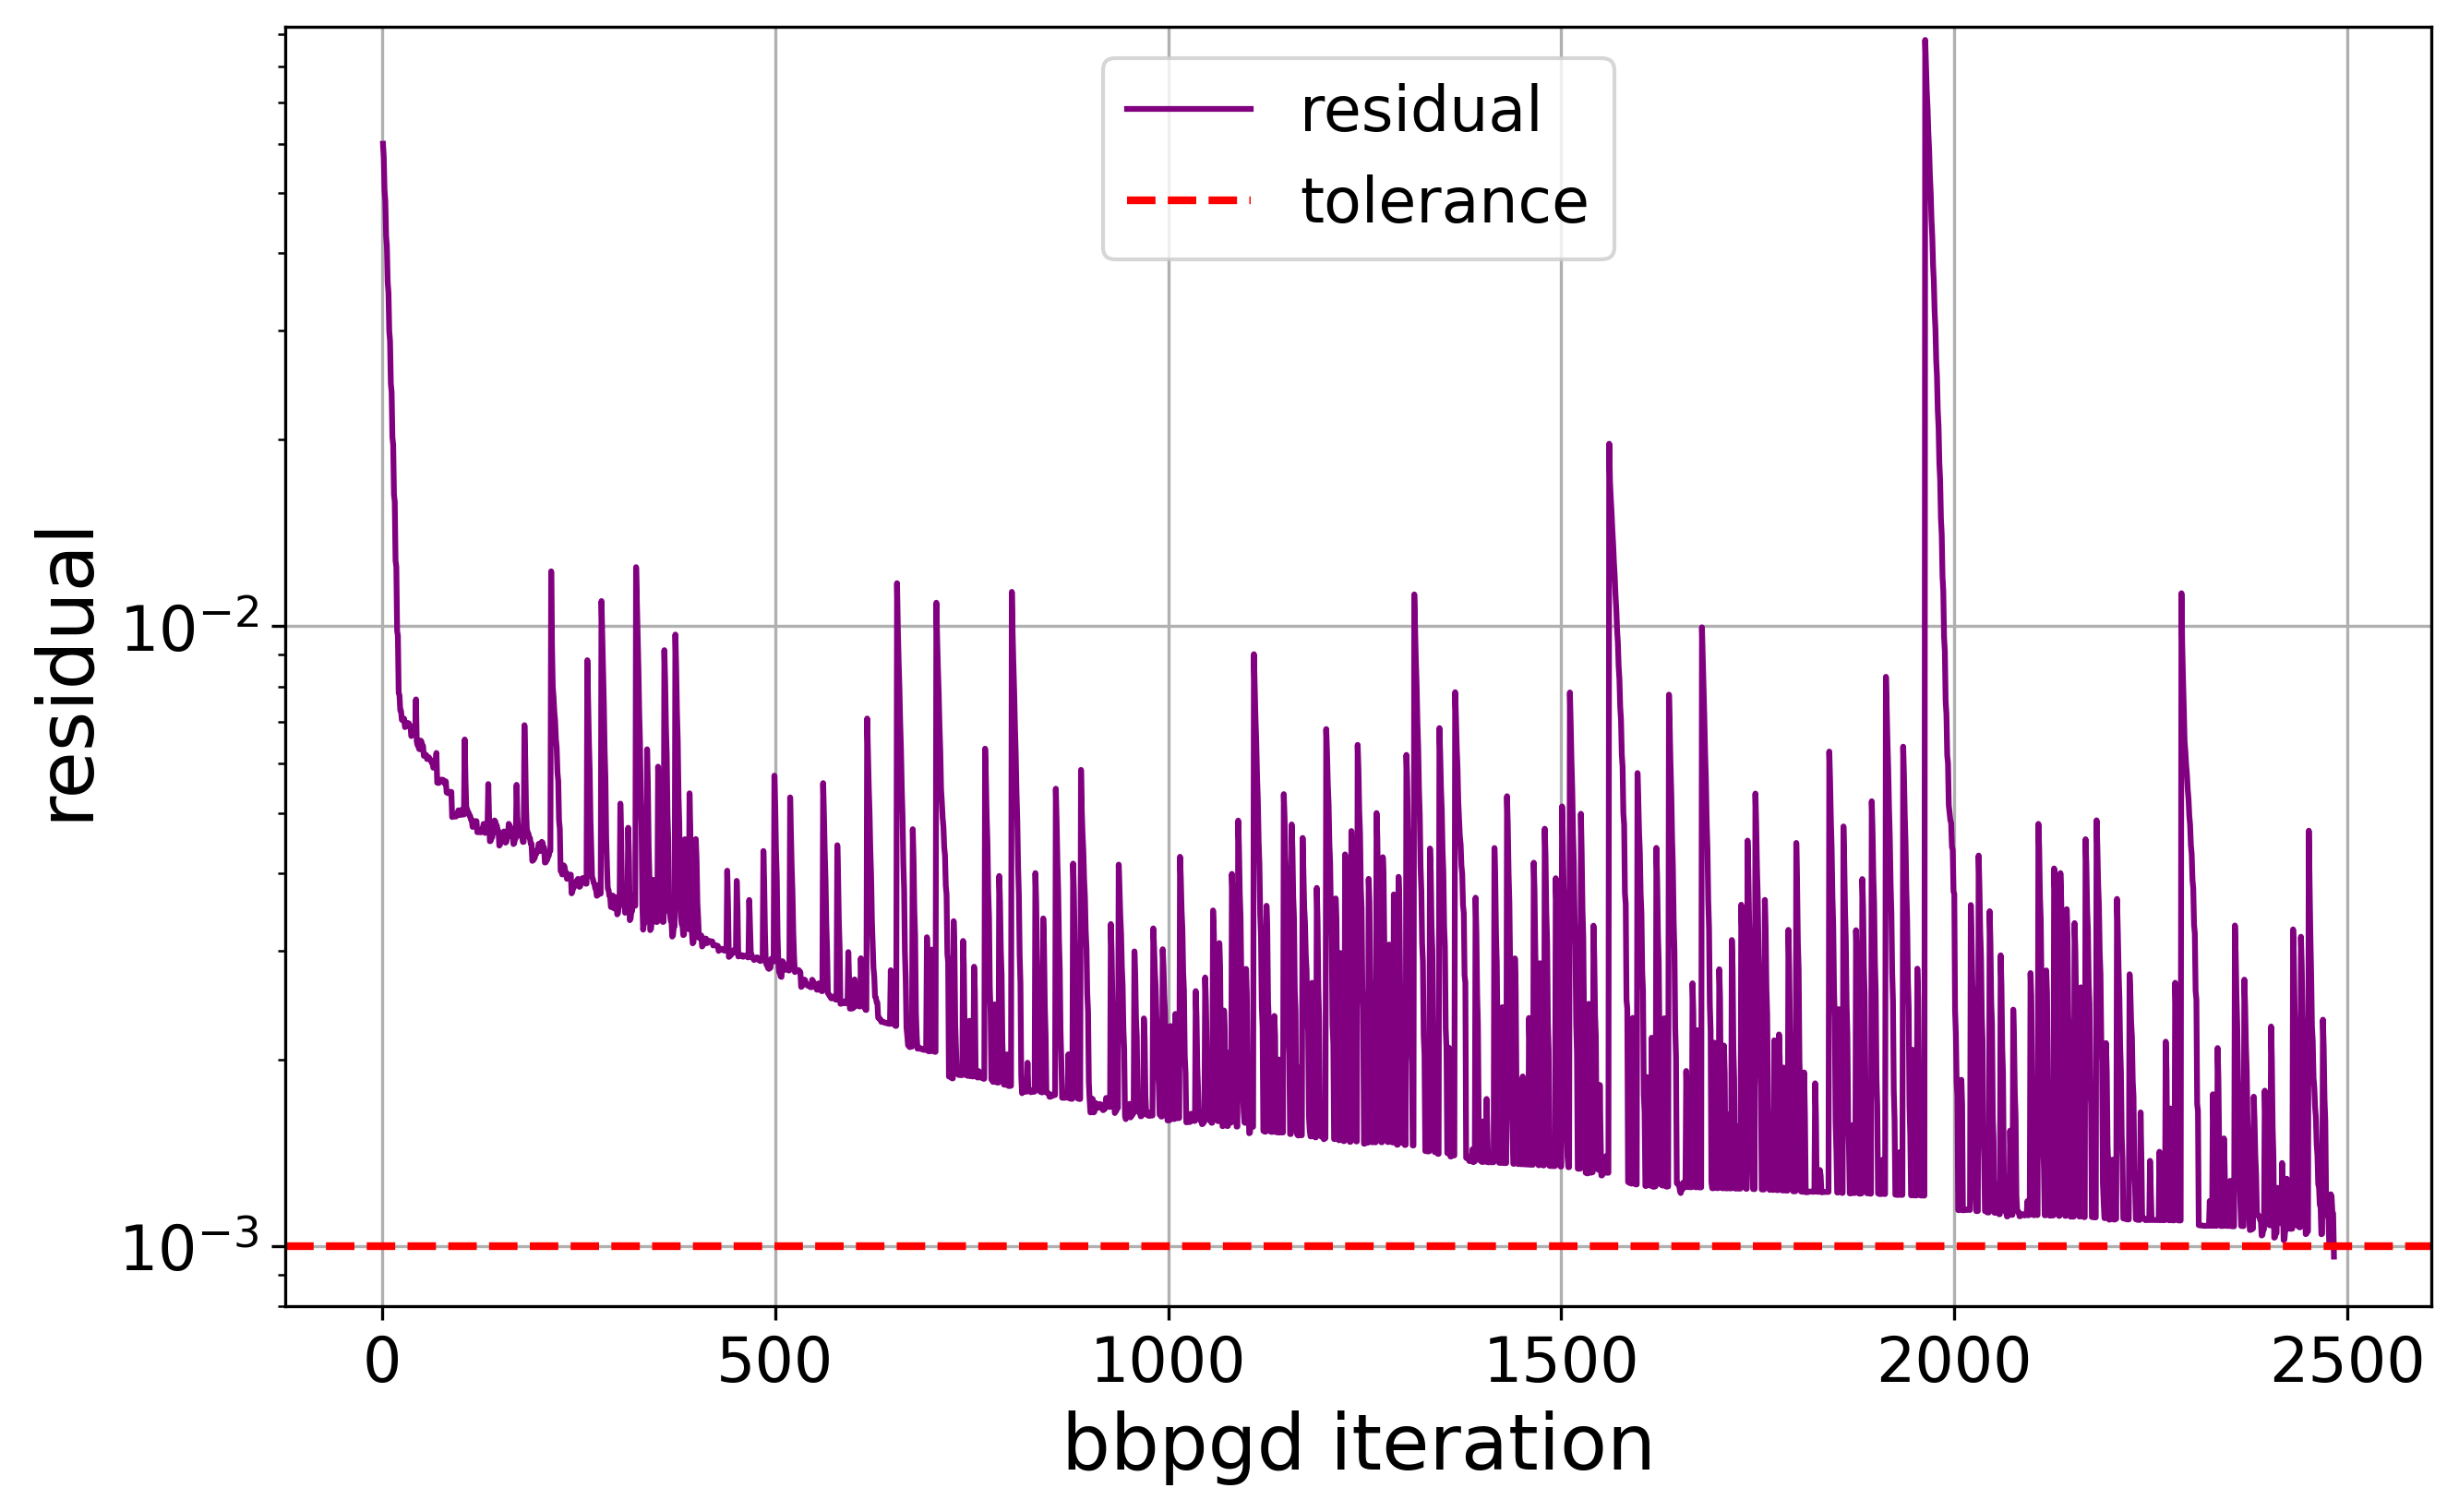
\includegraphics[width=\linewidth]{figures/comparison_plots/bbpgd_residual.png}
        \caption{BBPGD algorithm residuals over iterations for a single time step. The solver converges to the desired tolerance of $10^{-3}$ within about 2500 iterations.}
        \label{fig:bbpgd_residual}
    \end{subfigure}


    \begin{subfigure}[b]{\linewidth}
        \centering
        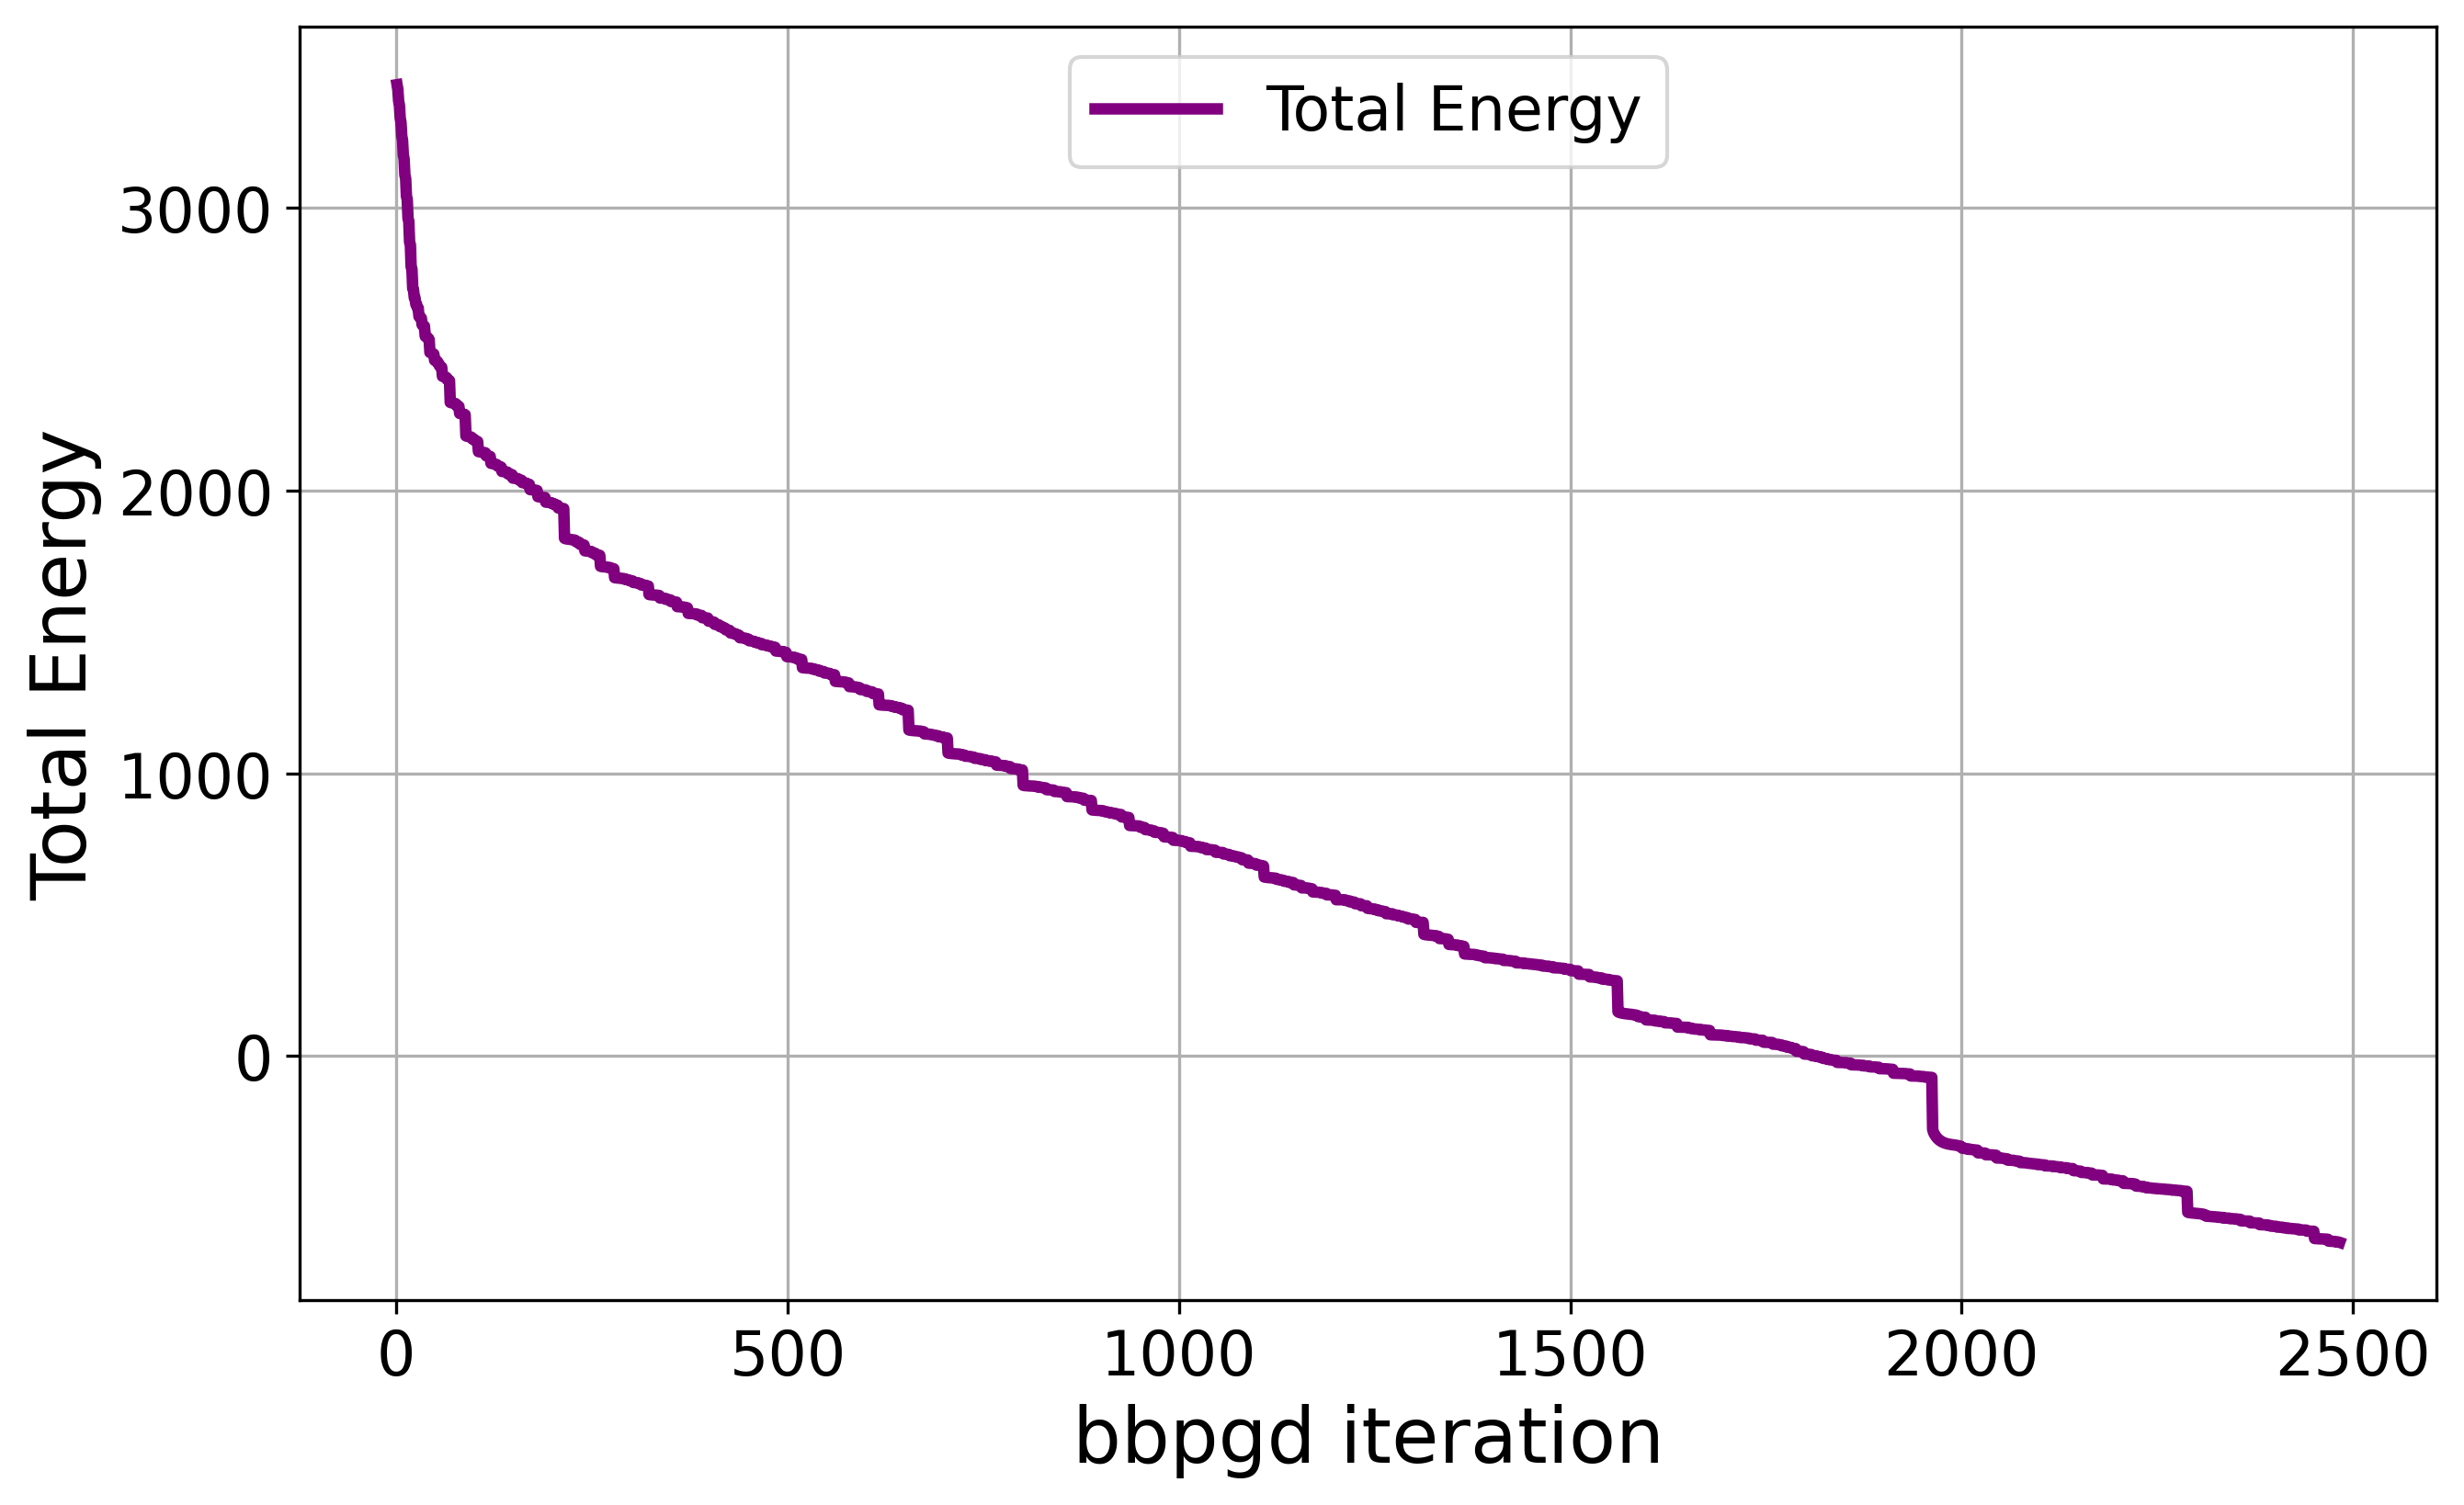
\includegraphics[width=\linewidth]{figures/comparison_plots/bbpgd_total_energy.png}
        \caption{System Energy value as described in \autoref{eq:energy_function} throughout the bbpgd algorithm. The energy decreases monotonically, confirming the convergence of the BBPGD method based on the projected gradient.}
        \label{fig:bbpgd_energy}
    \end{subfigure}

    \caption{BBPGD algorithm behavior during a single time step and across a full simulation.}
\end{figure}

\clearpage
\newpage







\newpage
\clearpage

\section{Discussion}

\subsection{Model Selection Insights}

The choice between hard and soft collision models involves a clear trade-off between physical fidelity and computational efficiency.
The hard model enforces strict non-overlap, which can be useful for capturing precise mechanical interactions or stress distributions in densely packed cell populations. However, it comes at considerable computational cost, requiring iterative global solvers and limiting scalability to large systems or long simulations.

By contrast, the soft model uses continuous repulsive potentials to approximate collisions. This approach is computationally efficient and scalable, making it well-suited for exploring large colonies or wide parameter spaces.

Importantly, for many emergent pattern-formation scenarios, such as concentric ring formation, the exact enforcement of non-overlap seems less critical. Other factors, such as stress-dependent growth and a use of an adequate time step, appear to dominate the macroscopic behavior.

In this context, the soft model provides a realistic approximation of cellular interactions: biological cells are deformable, and mechanical interactions in vivo are rarely perfectly rigid. Indeed, recent studies~\cite{Khan_2024, Ghosh2015, SantosDiaz2025} suggest that finite stiffness or soft repulsive forces are sufficient to capture key structural and morphological features of growing bacterial colonies.

\subsection{Biological Relevance}

Our results indicate that the soft collision model successfully reproduces major emergent patterns despite its simplified mechanics. This aligns with the view that colony-level behaviors are robust to the details of individual cell interactions, provided that key features like stress-dependent growth are captured.

Furthermore, the soft model naturally represents continuous pressure and proximity effects, which are biologically more plausible than instantaneous, perfectly rigid constraints. This makes it a compelling choice for simulating biological systems where cells exhibit elasticity and deformability.

\section{Conclusion}

This paper demonstrates that a computationally efficient soft collision model can reproduce complex emergent patterns in proliferating cell collectives, including concentric rings observed in bacterial colonies.

While hard collision models offer exact non-overlap and may be valuable when studying precise mechanical stresses or jamming phenomena, they are computationally intensive and less scalable. Soft models, using finite repulsion to approximate contact interactions, achieve a realistic balance between biological plausibility and computational performance.

\newpage
\section{Future Work}

The current implementation provides a functional baseline for hard collision modeling, yet significant opportunities exist for performance optimization in the constraint solver.

\subsection{Hard Collision Model}
The present PETSc-based implementation of the ReLCP constraint solver faces computational bottlenecks that limit its scalability, primarily due to dynamic memory management strategies for constraint matrices and vectors. While an allocation factor mitigates frequent reallocations, sudden increases in collision events still trigger costly memory recopies. Furthermore, allocated memory is not reused between solver iterations, necessitating complete cleanup and reallocation at each time step.

Future work should focus on developing a more sophisticated memory management strategy that leverages PETSc's advanced features, such as memory pooling for constraint matrices and vectors, matrix preallocation routines with accurate nonzero pattern prediction, and incremental growth strategies to minimize MPI synchronization overhead.


\subsection{GPU Acceleration}

\cite{Tasora2008}

\subsection{Soft Collision Model}

Beyond optimizing the hard model's solver, a promising avenue is the acceleration of the soft model using advanced molecular dynamics techniques. Libraries like AutoPas~\cite{AutoPasGithub,Gratl2019,Newcome2023} offer a node-level auto-tuning framework specifically designed for particle simulations.AutoPas can dynamically select the optimal combination of algorithms (e.g., for particle interaction traversal and container data structures) tailored to the specific simulation scenario and underlying hardware architecture.

Integrating such a framework could automatically accelerate the computation of repulsive forces in the soft collision model, especially for large-scale colonies where efficient neighbor-search and force evaluation are critical.

\newpage

\balance
\bibliographystyle{IEEEtran}
\bibliography{literature}
\newpage
\nobalance



\onecolumn

\appendix

\renewcommand{\thefigure}{A\arabic{figure}}
\renewcommand{\thetable}{A.\arabic{table}}
\setcounter{figure}{0}
\setcounter{table}{0}



\begin{figure}[H]
    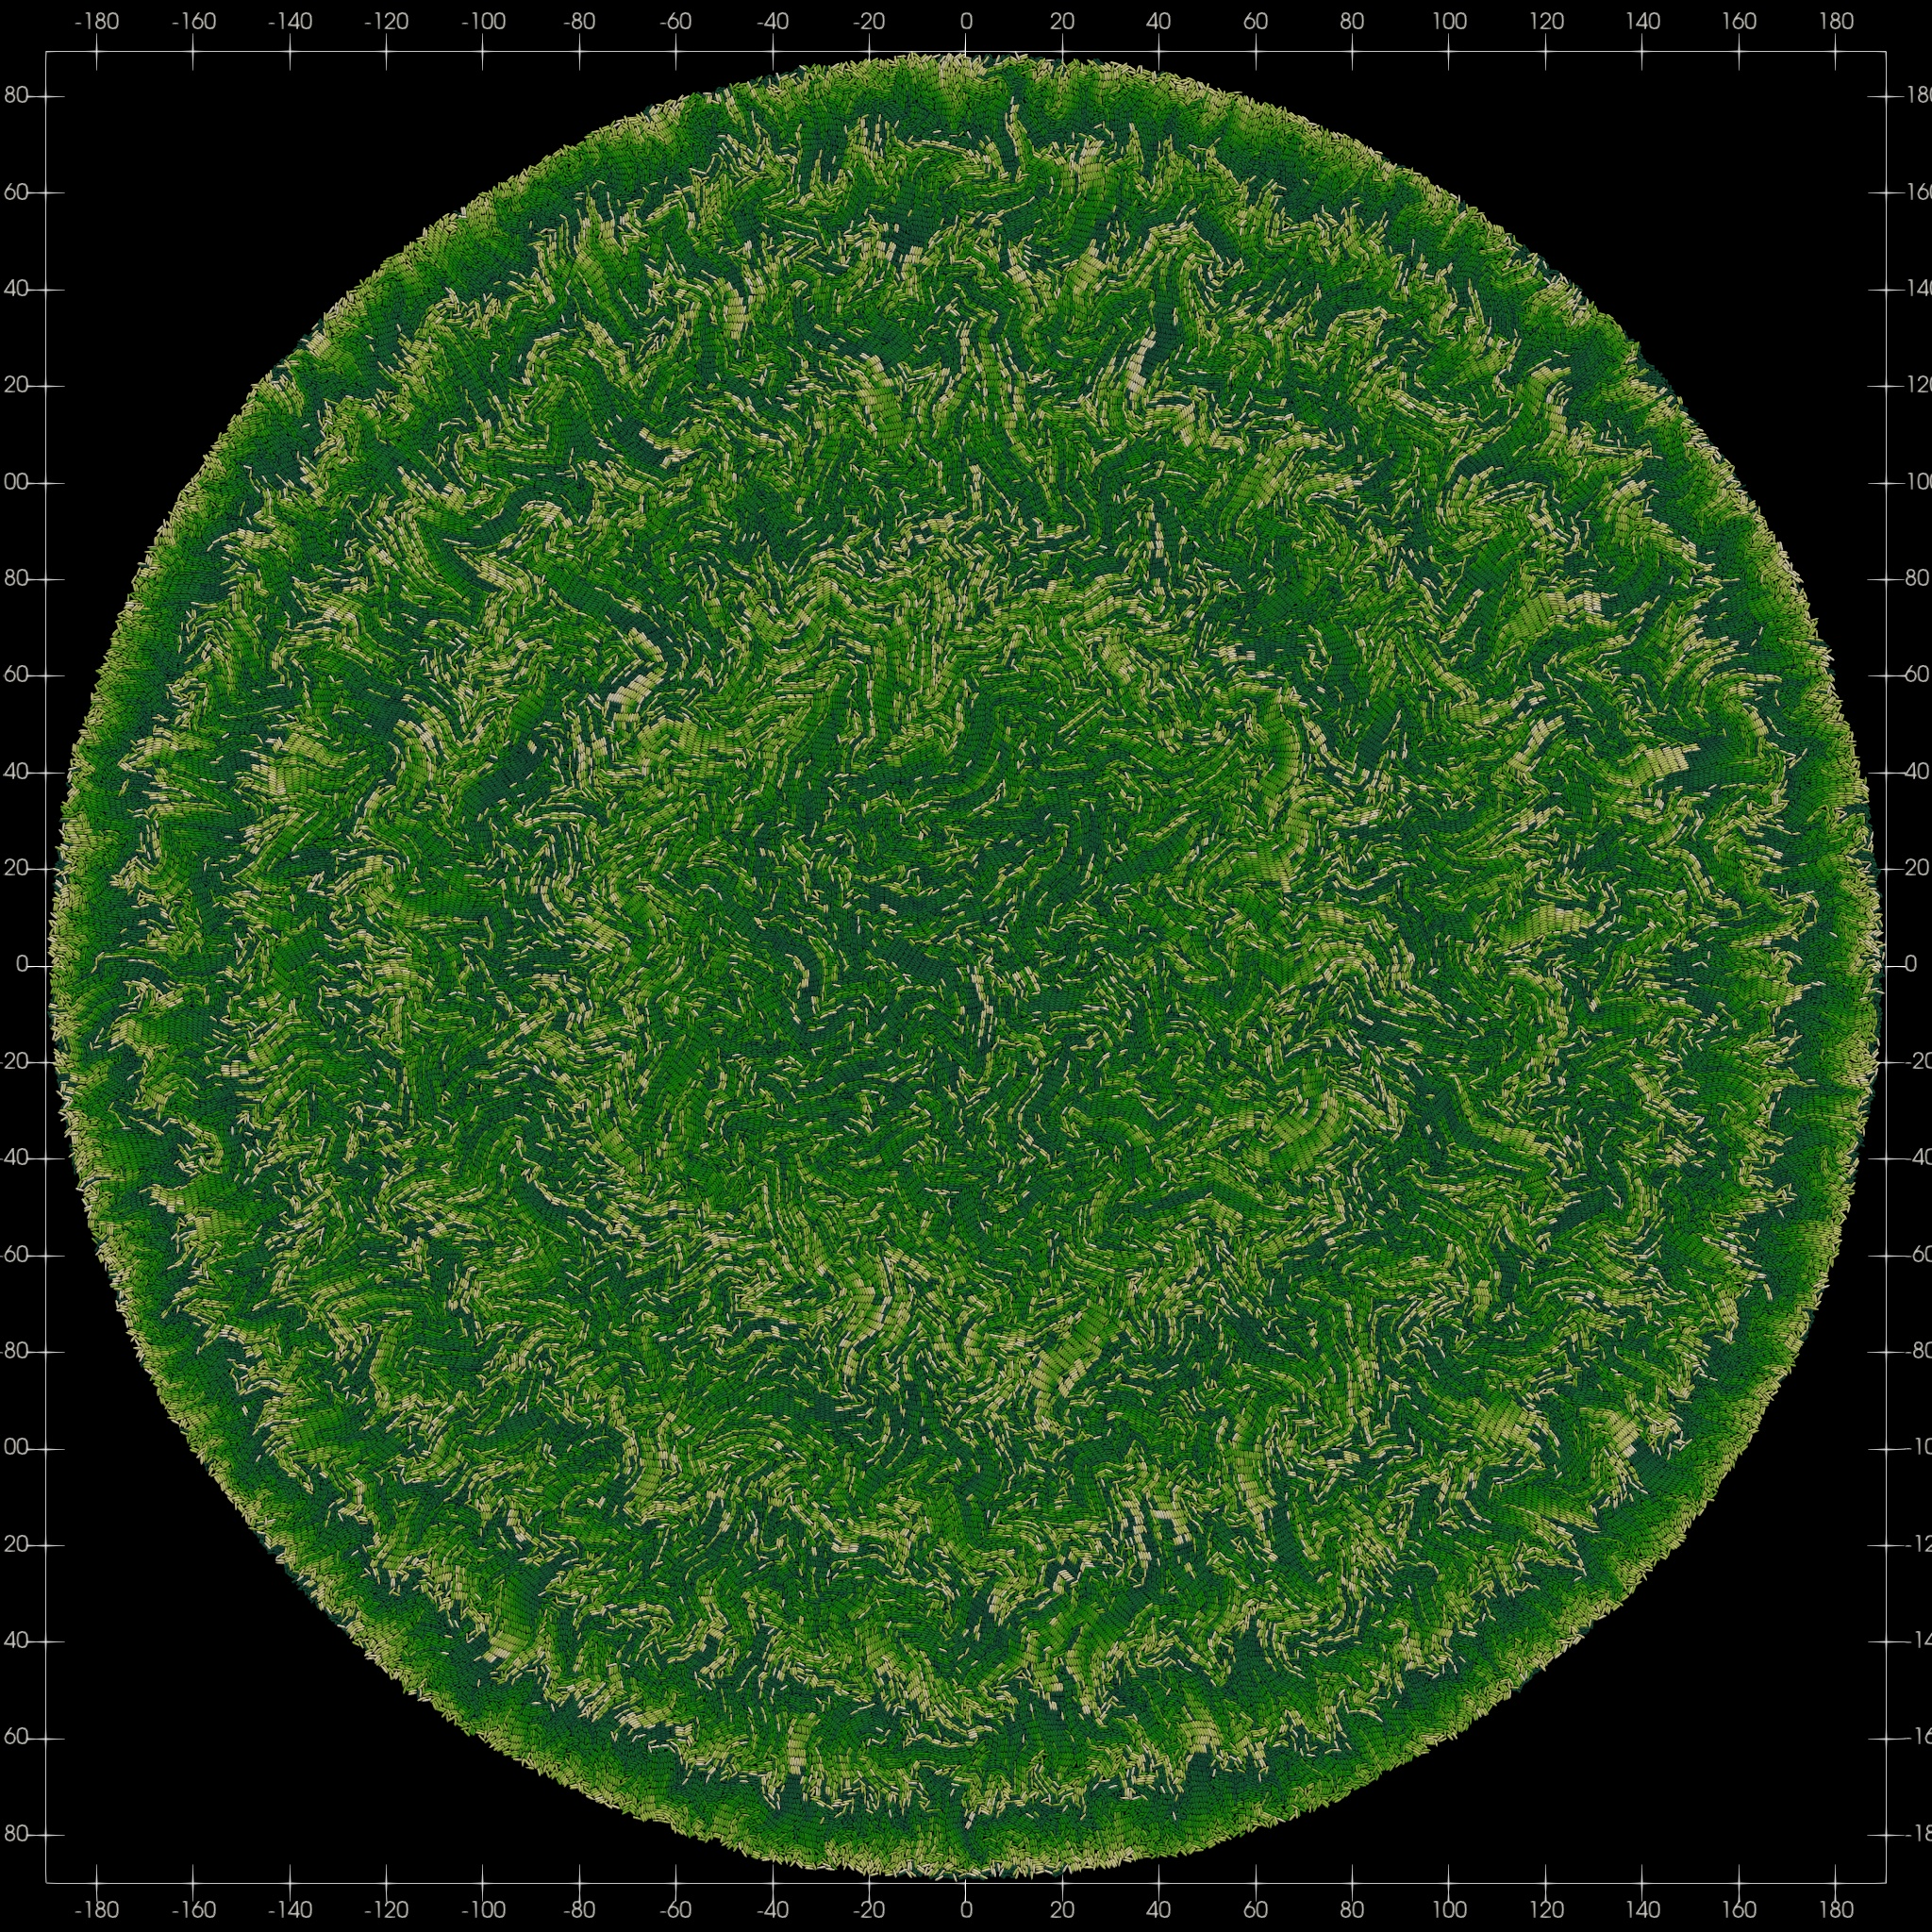
\includegraphics[width=\linewidth]{figures/growth/huge.jpeg}

    \caption{Snapshot of largest attainable colony size using the hard collision model with $\lambda=10^{-3}$ after 24h of wall time on 112 ranks on the CoolMUC-4 cluster. The colony has a radius of approximately $R \approx 195$ and consists of $168{,}339$ cells. The color indicates the length of the cells (short cells are darker, longer cells are lighter). Clear concentric ring patterns are visible, similar to those observed in smaller colonies (See \autoref{fig:pattern_formation}).}
    \label{fig:huge_colony_hard}
\end{figure}




\newpage



\clearpage
\newpage
\twocolumn
\tableofcontents

\end{document}